%%%%%%%%%%%%%%%%%%%%%%%%%%%%%%%%%%%%%%%%%%%%%%%%%%%%%%%%%%%%%%%
%
% Welcome to Overleaf --- just edit your LaTeX on the left,
% and we'll compile it for you on the right. If you open the
% 'Share' menu, you can invite other users to edit at the same
% time. See www.overleaf.com/learn for more info. Enjoy!
%
%%%%%%%%%%%%%%%%%%%%%%%%%%%%%%%%%%%%%%%%%%%%%%%%%%%%%%%%%%%%%%%
\documentclass[12pt,a4paper,oneside]{book}


\usepackage[T1]{fontenc}
\usepackage[utf8]{inputenc}
\usepackage{arabtex}
\usepackage{utf8}
\setcode{utf8}
\usepackage[shorthands=off,french,english]{babel} % English hyphenation for the report, French for the Résumé (no active characters, for arabtex)
\usepackage{svg}
\usepackage{amsmath}
\usepackage{amsthm}
\usepackage{amssymb}
\usepackage{tikz}
\usepackage{tcolorbox}
\usepackage{tabularx}
\usetikzlibrary{calc}
\usepackage[french,ruled,vlined]{algorithm2e}
\usepackage{rotating}
\usepackage{bbding}
\usepackage{cite}
\usepackage{lscape,graphicx}
\usepackage{rotating}
\usepackage{setspace}
\usepackage{sectsty}
\usepackage{dsfont}
\usepackage{ifpdf}
\usepackage{subfigure}
\usepackage{epsfig}
\usepackage{float}
\usepackage{titlesec}
\usepackage{multibib}
\usepackage{fancyhdr}
\usepackage{lipsum}
\usepackage{soul}
\usepackage[paperwidth=210mm,paperheight=297mm,tmargin=15mm,lmargin=20mm]{geometry}
%
\renewcommand{\topfraction}{0.9}
\renewcommand{\textfraction}{0.1}
\renewcommand{\floatpagefraction}{0.8}
%

\usepackage{hyperref}


\urlstyle{same}

\setlength{\headheight}{30pt}
\pagestyle{fancy}% \renewcommand{\chaptermark}[1]{\markboth{#1}{}}
\renewcommand{\chaptermark}[1]{\markboth{\MakeUppercase{#1}}{}}
\renewcommand{\sectionmark}[1]{\markright{\MakeUppercase{\thesection.\ #1}}}


%
% \renewcommand{\sectionmark}[1]{\markright{#1}}
%\renewcommand \thesection{\Roman{section}.}
%\renewcommand \thesubsection{\alph{subsection}.}
%
%\newcommand{\helv}{%
%\fontfamily\fontsize{9}{11}\selectfont}

%

% Clear Header Style on the Last Empty Odd pages
\makeatletter
  \def\cleardoublepage{\clearpage\if@twoside \ifodd\c@page\else%
      \hbox{}%
       \thispagestyle{empty}%              % Empty header styles
       \newpage%
       \if@twocolumn\hbox{}\newpage\fi\fi\fi}
\makeatother


\fancyhead[RE]{\textit{\nouppercase{\leftmark}}}
\fancyhead[LO]{\textit{\nouppercase{\rightmark}}}
\fancyhead[LE,RO]{\thepage}

\renewcommand{\headrulewidth}{0pt}
\renewcommand{\footrulewidth}{0pt}
%
\setcounter{secnumdepth}{4}
\setcounter{tocdepth}{4}
%

%
\def\ds{\displaystyle}
\def\dir{./figures}

%


%\setlength\topmargin{0in}
%\setlength\topmargin{0in}
%

%
% Remove page numbering from first page Bibliography
%
%%%%%%%%%%%%%%%%%%%%%%%%% Page de titre %%%%%%%%%%%%%%%%%%%%%%%
\def\baselinestretch{1.5}
% extra stretch only for paragraphs that would otherwise run into the margin
\setlength{\emergencystretch}{2em}


\usepackage{listings}
\usepackage{caption}
\usepackage{longtable}

\usepackage{geometry}
\usepackage{booktabs}

\geometry{
    letterpaper,
    left=1.5cm,
    right=1.5cm,
    top=1.5cm,
    bottom=1.5cm
}

\usepackage{afterpage}

\newcommand\blankpage{%
    \null
    \thispagestyle{empty}%
    \addtocounter{page}{-1}%
    \newpage}


\usepackage[acronym]{glossaries}

\usepackage{lmodern}


\newenvironment{dedication}
  {%\clearpage           % we want a new page          %% I commented this
   \thispagestyle{empty}% no header and footer
   \vspace*{\stretch{1}}% some space at the top
   \itshape             % the text is in italics
   \raggedleft          % flush to the right margin
  }
  {\par % end the paragraph
   \vspace{\stretch{3}} % space at bottom is three times that at the top
   \clearpage           % finish off the page
  }


  



%\makenoidxglossaries 

%\newglossaryentry{latex}
%{
       % name=latex,
        %description={Is a mark up language specially suited for scientific documents}
%}



%\selectlanguage{English}



\hypersetup{
    colorlinks=true,
    linkcolor=black,
    filecolor=magenta,      
    urlcolor=cyan,
    pdfauthor={Oualid AMTOUT},
    pdftitle={Design and Development of an AI-Powered Recruitment Platform Built on SAP BTP using ABAP RAP},
    pdfpagemode=FullScreen,
    }



\begin{document}



\definecolor{codegreen}{rgb}{0,0.6,0}
    \definecolor{codegray}{rgb}{0.5,0.5,0.5}
    \definecolor{codepurple}{rgb}{0.58,0,0.82}
    \definecolor{backcolour}{rgb}{0.95,0.95,0.92}
    
    \lstdefinestyle{mystyle}{
        backgroundcolor=\color{backcolour},   
        keywordstyle=\color{magenta},
        numberstyle=\tiny\color{codegreen},
        stringstyle=\color{codepurple},
        basicstyle=\ttfamily\footnotesize,
        breakatwhitespace=false,         
        breaklines=true,                 
        captionpos=b,                    
        keepspaces=true,                 
        numbers=left,                    
        numbersep=5pt,                  
        showspaces=false,                
        showstringspaces=false,
        showtabs=false,                  
        tabsize=2
    }




%
\thispagestyle{empty}

\includegraphics[scale=0.08]{Logos/Logo_INPT.png} 
         \hspace{11cm}  

\includegraphics[scale=0.1]{Logos/Logo_ANRT.jpg}
        
\vspace{0.9cm}
\begin{center}
{\large \textsc{\textbf{Mémoire du projet de fin d'études}}}\\[0.1cm]
{\large \textsc{Pour L'obtention du Diplôme d'Ingénieur d'État}}\\[0.1cm]
{\large \textsc{\textit{Filière: XXXXXXXXXXXX}}} \\[0.05cm] 
\vspace{-0.04cm}
% Title
\rule{\linewidth}{0.3mm} \\[0.4cm]   % à ajuster l'éspace en cas de besoin: [1cm]
 { \huge \textbf{ Titre de Projet }} \\[0.15cm] 
\rule{\linewidth}{0.3mm} \\[0.4cm]
\vspace{0.4cm}


\includegraphics[scale=0.075]{Logos/Company_Logo_Expl.png}  %change the scale to suit your logo

\vspace{1cm}

% Author and supervisor
\noindent
\begin{minipage}{0.9\textwidth}
    \vspace{-7mm}
  \begin{flushleft} \large
    \emph{Réalisé par :}\\
    Mme / M. Xxxx \textsc{XXXX} %\& Mme / M. Xxxx \textsc{XXXX}  %Au cas de binôme, remove the % \\
  \end{flushleft}
\end{minipage}
\begin{minipage}{0.4\textwidth}

\end{minipage}\\[0.6cm]

{\large \textit{Soutenu le XX Juillet 20XX, devant le jury composé de : }}\\[0.5cm]


\begin{tabular}{p{1cm}lll}
 & \large M / Mme. Xxxx \textsc{XXXX}  & \large INPT & \large - Examinateur/trice \\[0.1cm]
 & \large M / Mme. Xxxx \textsc{XXXX}  & \large INPT & \large - Examinateur/trice \\[0.1cm]
 & \large M / Mme. Xxxx \textsc{XXXX}  & \large INPT & \large - Encadrant/e \\[0.1cm]
  & \large M / Mme. Xxxx \textsc{XXXX}  & \large Entreprise & \large - Encadrant/e \\[0.1cm]
 
\end{tabular}

\vspace{0.5cm}

\includegraphics[scale=0.6]{Logos/ZLAFA.png}


\textsc{Agence National de Réglementation des Télécommunications}\\
\textsc{Institut National des Postes et Télécommunications}
% Bottom of the page

%\vspace{0.3cm}
{\large Promotion : 20XX/20XX}
   
\end{center}


 %FRENCH ONE


\thispagestyle{empty}

\includegraphics[scale=0.08]{Logos/Logo_INPT.png} 
         \hspace{11cm}  

\includegraphics[scale=0.1]{Logos/Logo_ANRT.jpg}
        
\vspace{0.6cm}
\begin{center}
{\large \textsc{\textbf{Internship Report
 }}}\\[0.1cm]
{\large \textsc{Module : Stage INE1}}\\[0.1cm]
{\large \textsc{\textit{Major: Advanced Software Engineering for Digital Services (ASEDS)
}}} \\[0.05cm] 
\vspace{-0.04cm}
% Title
\rule{\linewidth}{0.3mm} \\[0.4cm]   % à ajuster l'éspace en cas de besoin: [1cm]
 { \huge \textbf{ Design and Development of an AI-Powered Recruitment Platform Built on SAP BTP using ABAP RAP }} \\[0.15cm] 
\rule{\linewidth}{0.3mm} \\[0.4cm]


\includegraphics[scale=0.4]{Figures/logoCognitus.jpg}  %change the scale to suit your logo

\vspace{0.2cm}

% Author and supervisor
\noindent
\begin{minipage}{0.9\textwidth}
    \vspace{-7mm}
  \begin{flushleft} \large
    \emph{Authored by :}\\
   Oualid AMTOUT
 %\& Mr/Mrs/Ms. Xxxx \textsc{XXXX}  %Au cas de binôme, remove the % \\
  \end{flushleft}
\end{minipage}
\begin{minipage}{0.4\textwidth}

\end{minipage}\\[0.4cm]

{\large \textit{Supervised by :}}\\[0.5cm]


\begin{tabular}{p{1cm}lll}
 & \large Mr. \textsc{Karim Ait Alla}  & \large Cognitus & \large - Encadrant \\[0.1cm]
 
 
\end{tabular}

\vspace{0.4cm}

\includegraphics[scale=0.5]{Logos/ZLAFA.png}


\textsc{Agence Nationale de Réglementation des Télécommunications}\\
\textsc{Institut National des Postes et Télécommunications}
% Bottom of the page

%\vspace{0.3cm}
{\large Academic Year : 2025/2026}
   
\end{center}


 % ENGLISH

\afterpage{\blankpage}  %page vide obligatoire

\frontmatter


\chapter*{Dedication}
\addcontentsline{toc}{chapter}{Dedication}

\begin{dedication}
\large
\textit{To my beloved parents,}\\
\normalsize
Whose unconditional love, continuous sacrifices, and prayers have guided my path and inspired me to strive for excellence. Words cannot express my deepest gratitude for everything you have given me.
\par
\vspace{1.5\baselineskip}

\large
\textit{To my family, brothers, and sisters,}\\
\normalsize
For your unwavering support, continuous encouragement, and belief in my potential throughout my academic journey.
\par
\vspace{1.5\baselineskip}

\large
\textit{To my mentors, professors, and dear friends,}\\
\normalsize
Whose valuable insights, camaraderie, and encouragement have enriched both my personal and professional growth.
\par
\vspace{2\baselineskip}

\raggedleft
\large \textbf{Oualid AMTOUT}
\end{dedication}



\chapter*{Acknowledgments}
\addcontentsline{toc}{chapter}{Acknowledgments}

\noindent
First and foremost, I would like to express my deepest gratitude to Almighty God for granting me the strength, perseverance, and health to successfully complete this internship and realize this project.

\vspace{0.4cm}
\noindent
I would like to convey my sincere and profound gratitude to \textbf{Cognitus Corporation} for welcoming me into their team in Tangier and providing an intellectually stimulating, collaborative, and professional environment throughout my summer internship.

\vspace{0.4cm}
\noindent
I extend my heartfelt gratitude to my industrial supervisor, \textbf{Mr.\ Karim A\"it Alla}, Technical Lead at Cognitus, for the invaluable guidance, technical oversight, and regular follow-ups provided throughout the various stages of this project. The high standards and pragmatic feedback I received were instrumental in steering this work toward professional enterprise standards.

\vspace{0.4cm}
\noindent
I also express my sincere thanks to the members of the Cognitus team in Tangier for their time, availability, and generous support. They introduced me to the intricate and powerful world of enterprise ERP systems and pointed me to training tracks and learning resources that proved decisive in expanding my technical horizon. Thanks to their encouragement and constructive advice, I was able to rapidly acquire modern SAP development practices and to design and implement this solution.

\vspace{0.4cm}
\noindent
I also wish to thank the faculty of the \textbf{Advanced Software Engineering for Digital Services (ASEDS)} major at the \textbf{National Institute of Posts and Telecommunications (INPT)} for their high-quality pedagogy and continuous dedication to training skilled and rigorous engineers.

\vspace{0.4cm}
\noindent
Finally, I would like to extend my sincere appreciation to the honorable members of the jury for taking the time to evaluate this report and assess the fruits of this work.



\chapter*{Résumé}
\addcontentsline{toc}{chapter}{Résumé}

\begin{otherlanguage*}{french}
\enlargethispage{\baselineskip}% keeps the closing rule on the same page
Dans le paysage économique actuel, les entreprises modernes privilégient l'adoption d'un progiciel de gestion intégré (ERP) unique capable d'unifier et d'orchestrer l'ensemble de leurs fonctions opérationnelles, en particulier la gestion du capital humain (HCM). Conjointement, les avancées fulgurantes de l'intelligence artificielle (IA) et sa capacité d'analyse et de raisonnement sur des milliers de documents complexes ouvrent des perspectives inédites pour transformer les flux de recrutement et optimiser l'identification des meilleurs talents.

Réalisé au sein de Cognitus Corporation, ce rapport rend compte de mon stage d'initiation ingénieur effectué dans le cadre de la filière Advanced Software Engineering for Digital Services (ASEDS) à l'Institut National des Postes et Télécommunications (INPT). Constituant ma toute première immersion dans l'écosystème des systèmes d'information d'entreprise, cette expérience a débuté par une phase intensive de montée en compétences sur les technologies SAP modernes, fondée sur les cours officiels de SAP Learning : Exploring SAP Business Technology Platform, Learning Basic ABAP Programming et Building Transactional Apps with the ABAP RESTful Application Programming Model. Fort de ces acquis fondamentaux, j'ai entrepris le développement d'un projet applicatif complet selon les standards actuels de SAP.

La solution conçue fait le pont entre le recrutement externe et la gouvernance d'entreprise à travers une architecture à double facette : un portail web moderne et interactif dédié aux candidats, interconnecté à un environnement d'entreprise \textbf{SAP}. Ce socle permet aux gestionnaires RH de modéliser la structure organisationnelle, de publier des offres directement rattachées à des vacances de postes, et de piloter les candidatures via des pipelines d'évaluation structurés. Alimentée par un moteur d'IA pour le parsing sémantique des CV et développée avec \textbf{SAP ABAP RAP}, la plateforme assure une continuité fluide et automatisée depuis la présélection des profils jusqu'à la création de la fiche employé dans SAP.

\noindent\rule[2pt]{\textwidth}{0.5pt}

{\textbf{Mots clés :}}
ERP, Gestion du Capital Humain (HCM), SAP BTP, ABAP RAP, Clean Core, Intelligence Artificielle, Recrutement Intelligent, Structure Organisationnelle, React.
\\
\noindent\rule[2pt]{\textwidth}{0.5pt}\par
\end{otherlanguage*}

% \cleardoublepage
%

\chapter*{Summary}
\addcontentsline{toc}{chapter}{Summary}

In today's economic landscape, modern enterprises prioritize adopting a single Enterprise Resource Planning (ERP) system capable of unifying and orchestrating all operational functions, particularly Human Capital Management (HCM). Simultaneously, the remarkable advances in Artificial Intelligence (AI) and its ability to analyze and reason over thousands of complex documents open unprecedented avenues to transform recruitment workflows and optimize the identification of top talent.

Conducted at Cognitus Corporation, this report reflects my introductory engineering internship completed within the Advanced Software Engineering for Digital Services (ASEDS) major at the National Institute of Posts and Telecommunications (INPT). Representing my very first immersion into the enterprise information systems ecosystem, this experience began with an intensive upskilling phase on modern SAP technologies, based on the official SAP Learning courses: Exploring SAP Business Technology Platform, Learning Basic ABAP Programming, and Building Transactional Apps with the ABAP RESTful Application Programming Model. Building upon these fundamental skills, I undertook the development of a full-scale application following current SAP standards.

The resulting solution bridges external recruitment and corporate governance through a dual-faceted architecture: a modern and interactive web portal dedicated to candidates, interconnected with an enterprise \textbf{SAP} environment. This foundation enables HR managers to model organizational structure, publish job offers directly mapped to vacancies, and manage applications through structured evaluation pipelines. Powered by an AI engine for semantic resume parsing and built with \textbf{SAP ABAP RAP}, the platform ensures a smooth, automated continuum from candidate pre-selection to employee file creation in SAP.

\noindent\rule[2pt]{\textwidth}{0.5pt}

{\textbf{Key Words :}}
ERP, Human Capital Management (HCM), SAP BTP, ABAP RAP, Clean Core, Artificial Intelligence, Smart Recruitment, Organizational Structure, React.
\\
\noindent\rule[2pt]{\textwidth}{0.5pt}

% \cleardoublepage
%

\chapter*{\RL{ملخص}}
\addcontentsline{toc}{chapter}{Arabic Abstract}

\begin{RLtext}
\noindent
في المشهد الاقتصادي الحالي، تفضل الشركات الحديثة اعتماد نظام \L{ERP} موحد قادر على إدارة وتنسيق كافة وظائفها التشغيلية، ولا سيما إدارة الرأسمال البشري (\L{HCM}). وفي الوقت ذاته، تفتح التطورات المتسارعة للذكاء الاصطناعي (\L{AI}) وقدرته على تحليل آلاف الوثائق المعقدة آفاقا جديدة لتطوير عمليات التوظيف وانتقاء أفضل الكفاءات.

\vspace{0.3cm}
يقدم هذا التقرير، المنجز بشركة \L{Cognitus Corporation}، حصيلة تدريب المهندس ضمن مسلك \L{ASEDS} بالمعهد الوطني للبريد والمواصلات (\L{INPT}). وباعتباره أول تجربة لي في أنظمة المؤسسات، بدأت هذه المرحلة بتكوين مكثف في تقنيات \L{SAP} الحديثة من خلال دورات رسمية في منصة \L{BTP} وبرمجة \L{ABAP} ونموذج \L{RAP}، مما مكنني من تطوير مشروع تطبيقي متكامل وفق معايير \L{SAP} الحالية.

\vspace{0.3cm}
يربط النظام المطور بين التوظيف الخارجي وإدارة المؤسسة عبر بنية مزدوجة: بوابة \L{Web} حديثة للمترشحين، متصلة بنظام \L{SAP} الداخلي. وتتيح هذه المنظومة للمسؤولين نمذجة الهيكل التنظيمي، ونشر عروض العمل، وتتبع المترشحين عبر مراحل تقييم محددة. وبفضل محرك الذكاء الاصطناعي لتحليل السير الذاتية وتطويره باستخدام \L{SAP ABAP RAP}، يضمن النظام مسارا سلسا ومؤتمتا من الانتقاء الأولي حتى تسجيل الموظف في \L{SAP}.
\end{RLtext}

\noindent\rule[2pt]{\textwidth}{0.5pt}

\begin{RLtext} 
{\textbf{الكلمات المفتاحية :}}
نظام \L{ERP}، إدارة الرأسمال البشري (\L{HCM})، \L{SAP BTP}، \L{ABAP RAP}، الذكاء الاصطناعي، التوظيف الذكي، الهيكل التنظيمي، \L{React}.
\\
\end{RLtext}

\noindent\rule[2pt]{\textwidth}{0.5pt}

% \cleardoublepage
%






\listoffigures
\addcontentsline{toc}{chapter}{List of Figures} 
%figures are added automatically here

\listoftables
\addcontentsline{toc}{chapter}{List of Tables} 
%tables are added automatically here

\lstlistoflistings
\addcontentsline{toc}{chapter}{List of Listings} 
%Code snippets are added automatically here

\tableofcontents
\addcontentsline{toc}{chapter}{Table of Contents}
%contents are added automatically here

\mainmatter

%debut of chapters

\chapter{General Project Context}
\label{chap:General Project Context}

% ─────────────────────────────────────────────
\section*{Introduction}
\addcontentsline{toc}{section}{Introduction}
% ─────────────────────────────────────────────

I had the opportunity to complete my first internship at Cognitus Corporation, specifically within its Global Delivery and Support Center (GDSC) located in Tangier, Morocco. This experience constituted my very first immersion into the world of enterprise information systems, and more precisely into the SAP ecosystem. In the sections that follow, I will introduce Cognitus Corporation as a global organization, shed light on its Tangier office and its strategic role within the group, and then present the technical project I was entrusted with during this internship period.

\newpage

% ─────────────────────────────────────────────
\section{Cognitus Corporation}
% ─────────────────────────────────────────────

\subsection{About Cognitus Corporation}

\begin{figure}[H]
    \centering
    
\includegraphics[width=12cm]{Figures/logoCognitus.jpg}
    \caption{Cognitus Corporation Logo}
    \label{fig:cognitus_logo}
\end{figure}

Cognitus Corporation is a global SAP Gold Partner and a leading provider of cloud ERP implementations, SAP consulting, and digital transformation services. Founded with the mission of helping organizations unlock the full potential of SAP technology, Cognitus has built over two decades of deep industry expertise across more than eleven verticals, including manufacturing, public sector, retail, healthcare, and financial services.

The company offers a comprehensive range of SAP-centered services, spanning end-to-end implementation of SAP S/4HANA, RISE with SAP, and GROW with SAP programs, as well as specialized consulting in areas such as supply chain optimization, contract lifecycle management (CLM), and real-time billing. In addition to its consulting capabilities, Cognitus has developed a suite of proprietary AI-enabled software assets designed to accelerate data migration, automate compliance workflows in government contracting environments, and streamline business process transformation.

In 2025, Cognitus was acquired by IBM, reinforcing IBM's strategic position in the global SAP services market. This acquisition underscores Cognitus's standing as a recognized leader in RISE with SAP and GROW with SAP advisory, and consolidates its portfolio of accelerators and industry-specific SAP solutions within IBM's broader technology ecosystem.

Throughout its growth, Cognitus has maintained a strong commitment to delivering on-shore, off-shore, and nearshore support models, enabling clients around the world to maintain and continuously optimize their SAP environments in a cost-effective and agile manner.

\begin{figure}[H]
    \centering
    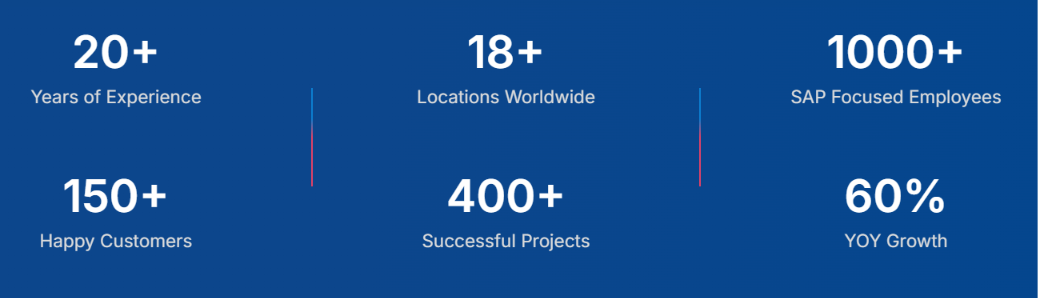
\includegraphics[width=12cm]{Figures/1.png}
    \caption{Cognitus Corporation --- Global Footprint}
    \label{fig:cognitus_global}
\end{figure}

\noindent
Cognitus operates across more than 18 global offices, with its headquarters in the United States and a strategic delivery center in Tangier, Morocco. The company serves over 150 enterprise clients, employs more than 1{,}000 SAP-focused specialists, and has successfully delivered over 400 SAP projects. Its model blends on-shore, off-shore, and nearshore delivery, offering clients both cost efficiency and cultural alignment across time zones.

\subsection{Cognitus Tangier --- Global Delivery and Support Center}

\begin{figure}[H]
    \centering
    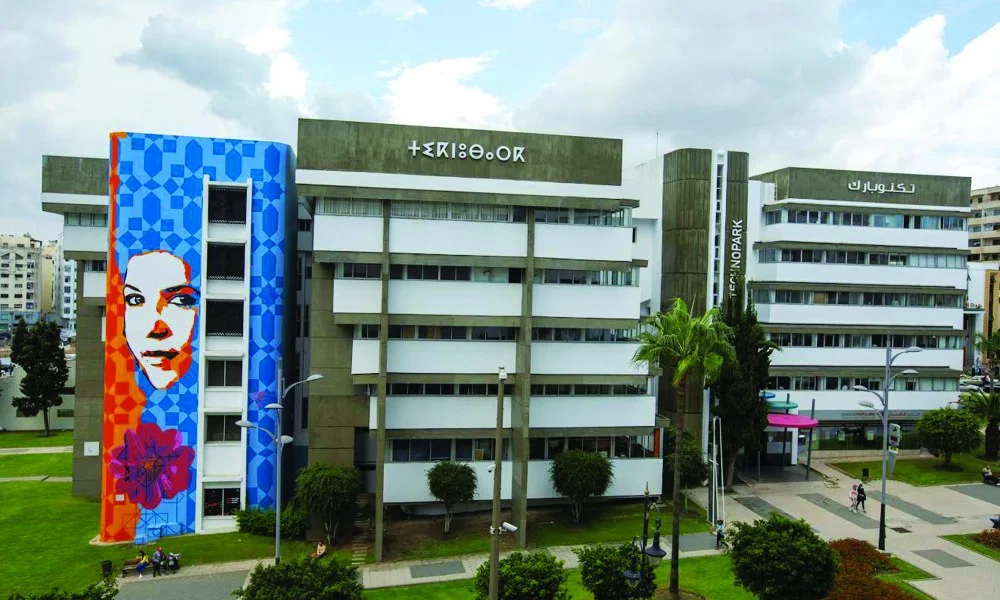
\includegraphics[width=12cm]{Figures/technoparcke.png}
    \caption{Cognitus Tangier --- Technopark, Avenue Mohammed V}
    \label{fig:technoparcke}
\end{figure}

Established in 2021, the Cognitus office in Tangier, Morocco serves as the company's Global Delivery and Support Center (GDSC) for the EMEA region and beyond. Strategically located at Technopark, Avenue Mohammed V, Tangier 90000, this center was designed to leverage the multilingual and highly skilled Moroccan talent pool --- capable of operating in French, Arabic, English, Spanish, and Italian --- to deliver seamless support and implementation services across different time zones.

The Tangier GDSC plays a pivotal role within the Cognitus global operations model. It functions as a nearshore hub that bridges the gap between client needs in Europe, the Middle East, Africa, and North America, and the delivery teams responsible for SAP system configuration, ABAP development, WRICEF object construction, testing, and post-go-live support.

Within this center, cross-functional teams collaborate on live SAP projects, supporting clients with S/4HANA implementations and custom extensions. The center embodies Cognitus's philosophy of combining global reach with localized expertise, offering clients the responsiveness and cultural alignment of a nearshore model with the cost efficiency typically associated with offshore delivery.

% ─────────────────────────────────────────────
\subsection{Business Area of Activity}
% ─────────────────────────────────────────────

Cognitus Corporation operates at the intersection of enterprise technology and business transformation, focusing exclusively on the SAP ecosystem. Its business activity is organized around four major pillars that together cover the full lifecycle of an SAP program:

\begin{itemize}
    \item \textbf{SAP Implementation \& Transformation:} End-to-end delivery of SAP programs, from initial assessment and blueprint design through go-live and hypercare. Cognitus specializes in \textit{RISE with SAP} (private cloud migrations) and \textit{GROW with SAP} (public cloud adoption for mid-market), leveraging pre-built industry templates to accelerate project timelines significantly.

    \item \textbf{Proprietary Accelerator Assets:} Cognitus distinguishes itself through a suite of SAP-endorsed, AI-enabled software products, including:
    \begin{itemize}
        \item \textit{CIS-GovCon} --- a government contracting compliance solution aligned with DCAA, DCMA, FAR, and CAS regulations;
        \item \textit{Contract Lifecycle Management (CLM)} --- an AI-powered tool automating contract authoring, approval, and monitoring;
        \item \textit{Data Migration Accelerator} --- a low-code, AI-assisted platform for migrating legacy data to S/4HANA;
        \item \textit{Real-Time Billing} --- an accelerator for project-based billing and revenue recognition.
    \end{itemize}

    \item \textbf{Application Management Services (AMS):} 24/7 system support, proactive optimization, basis administration, and performance monitoring for clients already on SAP, through on-shore, off-shore, and nearshore delivery models.

    \item \textbf{Strategic Consulting:} Assessment services, M\&A integration technology roadmaps, digital transformation strategy, and organizational change management aligned to SAP programs.
\end{itemize}

\textbf{Industries Served.}
Cognitus concentrates on sectors characterized by high operational complexity and regulatory requirements:

\begin{itemize}
    \item \textbf{Aerospace \& Defense} --- Government contracting, DCAA/DCMA compliance, MRP;
    \item \textbf{Manufacturing} --- Supply chain optimization, production planning, plant maintenance;
    \item \textbf{Life Sciences} --- Serialization, quality management, regulatory traceability;
    \item \textbf{Energy, Oil \& Gas} --- Asset management, project systems, real-time billing;
    \item \textbf{Professional Services} --- Project accounting, CLM, resource management;
    \item \textbf{Consumer Products} --- Demand planning, distribution, trade promotions;
    \item \textbf{Public Sector} --- Federal financials, grants management, GovCon compliance.
\end{itemize}

\textbf{Notable Clients.}
Among Cognitus's reference clients, several high-profile success stories illustrate the depth and speed of its delivery approach:

\begin{itemize}
    \item \textbf{Boom Supersonic} --- Implemented SAP S/4HANA in under three weeks to meet commercialization and regulatory compliance requirements;
    \item \textbf{Phlow Corporation} --- Adopted RISE with SAP to overcome siloed operations and stringent pharmaceutical regulatory requirements;
    \item \textbf{SunnySky Products} --- Standardized multi-site operations using SAP S/4HANA Public Cloud via the GROW with SAP program;
    \item \textbf{Volumetric Building Companies} --- Completed a full ERP modernization in three months using GROW with SAP Fast.
\end{itemize}

% ─────────────────────────────────────────────
\subsection{Enterprise Resource Planning (ERP)}
% ─────────────────────────────────────────────

\subsubsection{What is an ERP System?}

An \textbf{Enterprise Resource Planning (ERP)} system is an integrated suite of software applications designed to manage and automate an organization's core business processes across a single, unified platform. Rather than maintaining isolated systems for finance, procurement, human resources, manufacturing, and logistics, an ERP brings all these functions under one shared database and one coherent process model, enabling real-time visibility, consistent data, and end-to-end process automation across the enterprise.

The fundamental value proposition of an ERP system rests on three pillars:

\begin{enumerate}
    \item \textbf{Integration:} All business modules share a single source of truth. A sales order automatically triggers inventory checks, production planning, procurement, and financial accounting entries --- without any manual re-entry of data.
    \item \textbf{Standardization:} ERP systems enforce best-practice process models (often called \textit{business blueprints}) that align internal workflows with industry standards, reducing errors and audit risk.
    \item \textbf{Real-Time Visibility:} Decision-makers at all levels gain instant access to consolidated operational data, enabling faster and better-informed decisions.
\end{enumerate}

\begin{figure}[H]
    \centering
    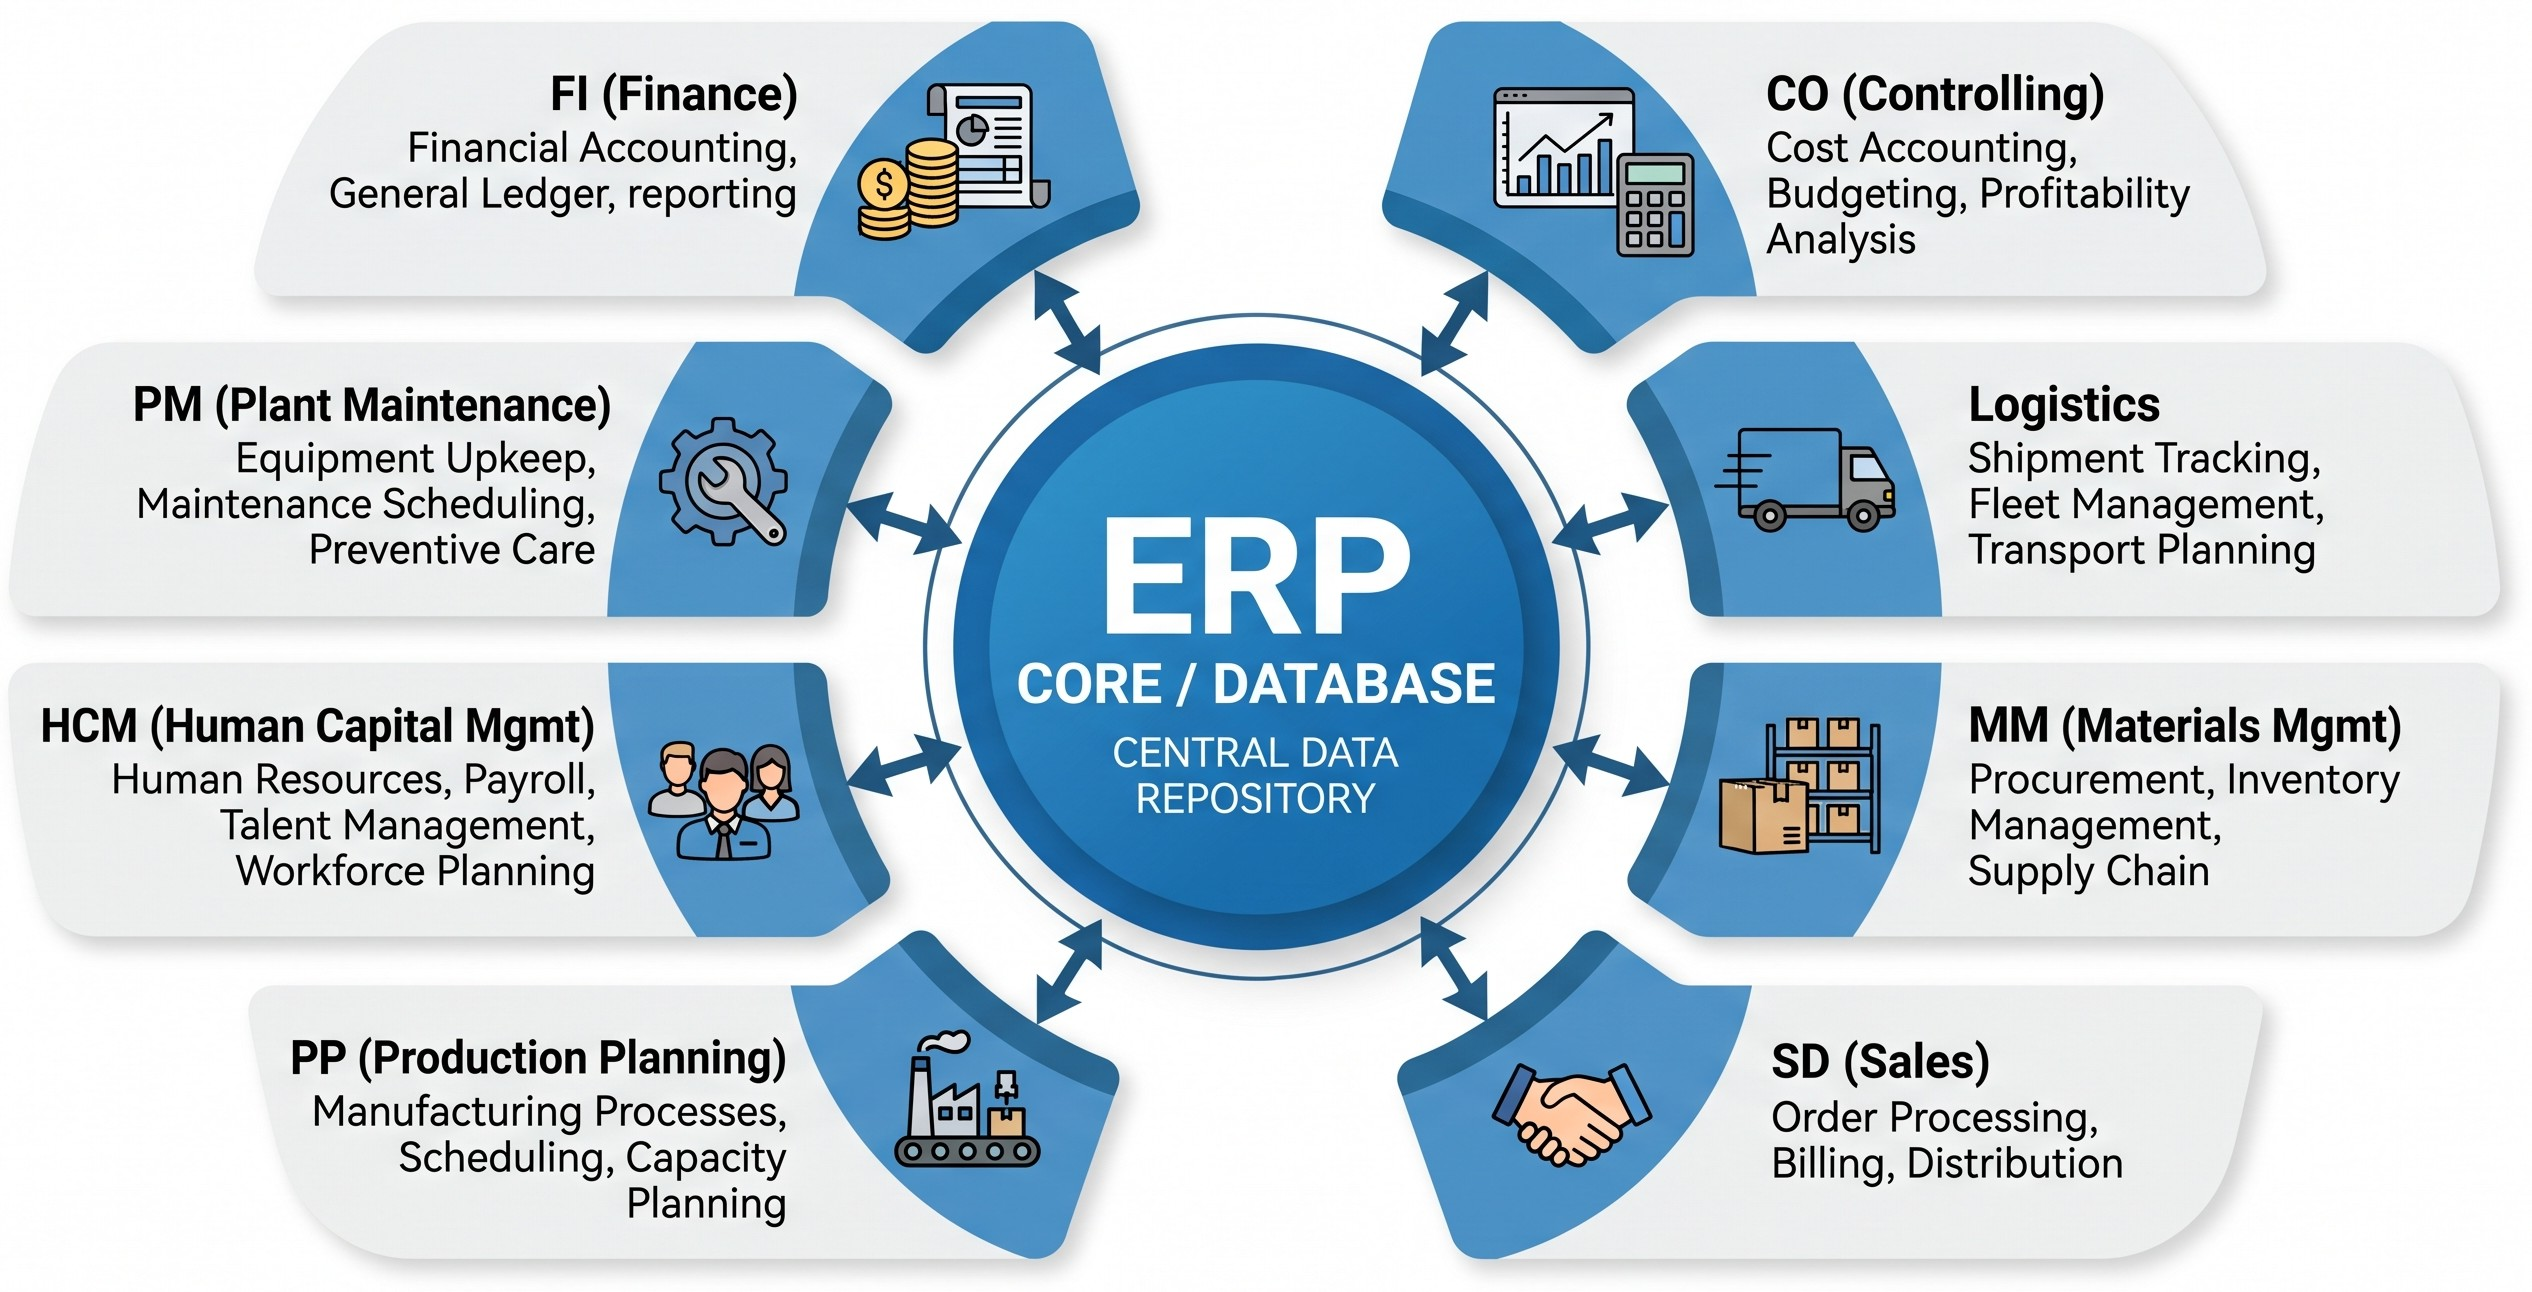
\includegraphics[width=15cm]{Figures/erp_modules.jpg}
    \caption{ERP System --- Integrated Business Module Architecture}
    \label{fig:erp_diagram}
\end{figure}

Modern ERP systems have evolved significantly since their origins in the 1960s--1970s. Early \textit{Material Requirements Planning (MRP)} systems focused solely on manufacturing inventory. The concept expanded in the 1990s into full \textit{ERP} suites covering the entire enterprise, and has since continued to evolve toward cloud-native, AI-augmented platforms capable of processing massive transactional volumes in real time.

In the context of this project, the ERP system at stake is the \textbf{SAP Human Capital Management (HCM)} module, which manages the organization's entire people-related data: employee master records, organizational structure, positions, and job offers. The web recruitment platform developed during this internship consumes and produces data within this SAP HCM layer through standard APIs.

% ─────────────────────────────────────────────
\subsection{SAP --- Systems, Applications, and Products}
% ─────────────────────────────────────────────

\subsubsection{SAP S/4HANA}

\textbf{SAP S/4HANA} is SAP's next-generation ERP suite, built natively on the \textbf{SAP HANA in-memory database}. Unlike its predecessor SAP ECC, S/4HANA delivers real-time transactional analytics, a simplified data model, and a modern web-based experience through \textbf{SAP Fiori}. It covers all core enterprise functions through dedicated modules --- notably \textbf{HCM} (Human Capital Management) for personnel administration, organizational management, and recruitment, which is the module at the heart of this project.

\subsubsection{SAP Business Technology Platform (BTP)}

\textbf{SAP BTP} is SAP's cloud-native \textit{Platform-as-a-Service (PaaS)}, designed to integrate, extend, and build applications across the SAP ecosystem. It unifies four capability areas: \textbf{Database \& Data Management} (HANA Cloud, Datasphere), \textbf{Analytics} (SAP Analytics Cloud), \textbf{Application Development \& Automation} (CAP, SAP Build), and \textbf{Integration} (SAP Integration Suite, API Management).

\subsubsection{ABAP and the RESTful Application Programming Model (RAP)}

\textbf{ABAP} (\textit{Advanced Business Application Programming}) is SAP's proprietary programming language, in use since the early 1980s. Its modern cloud-ready form is the \textbf{ABAP RESTful Application Programming Model (RAP)}, which structures development mainly in three clean layers:

\begin{figure}[H]
    \centering
    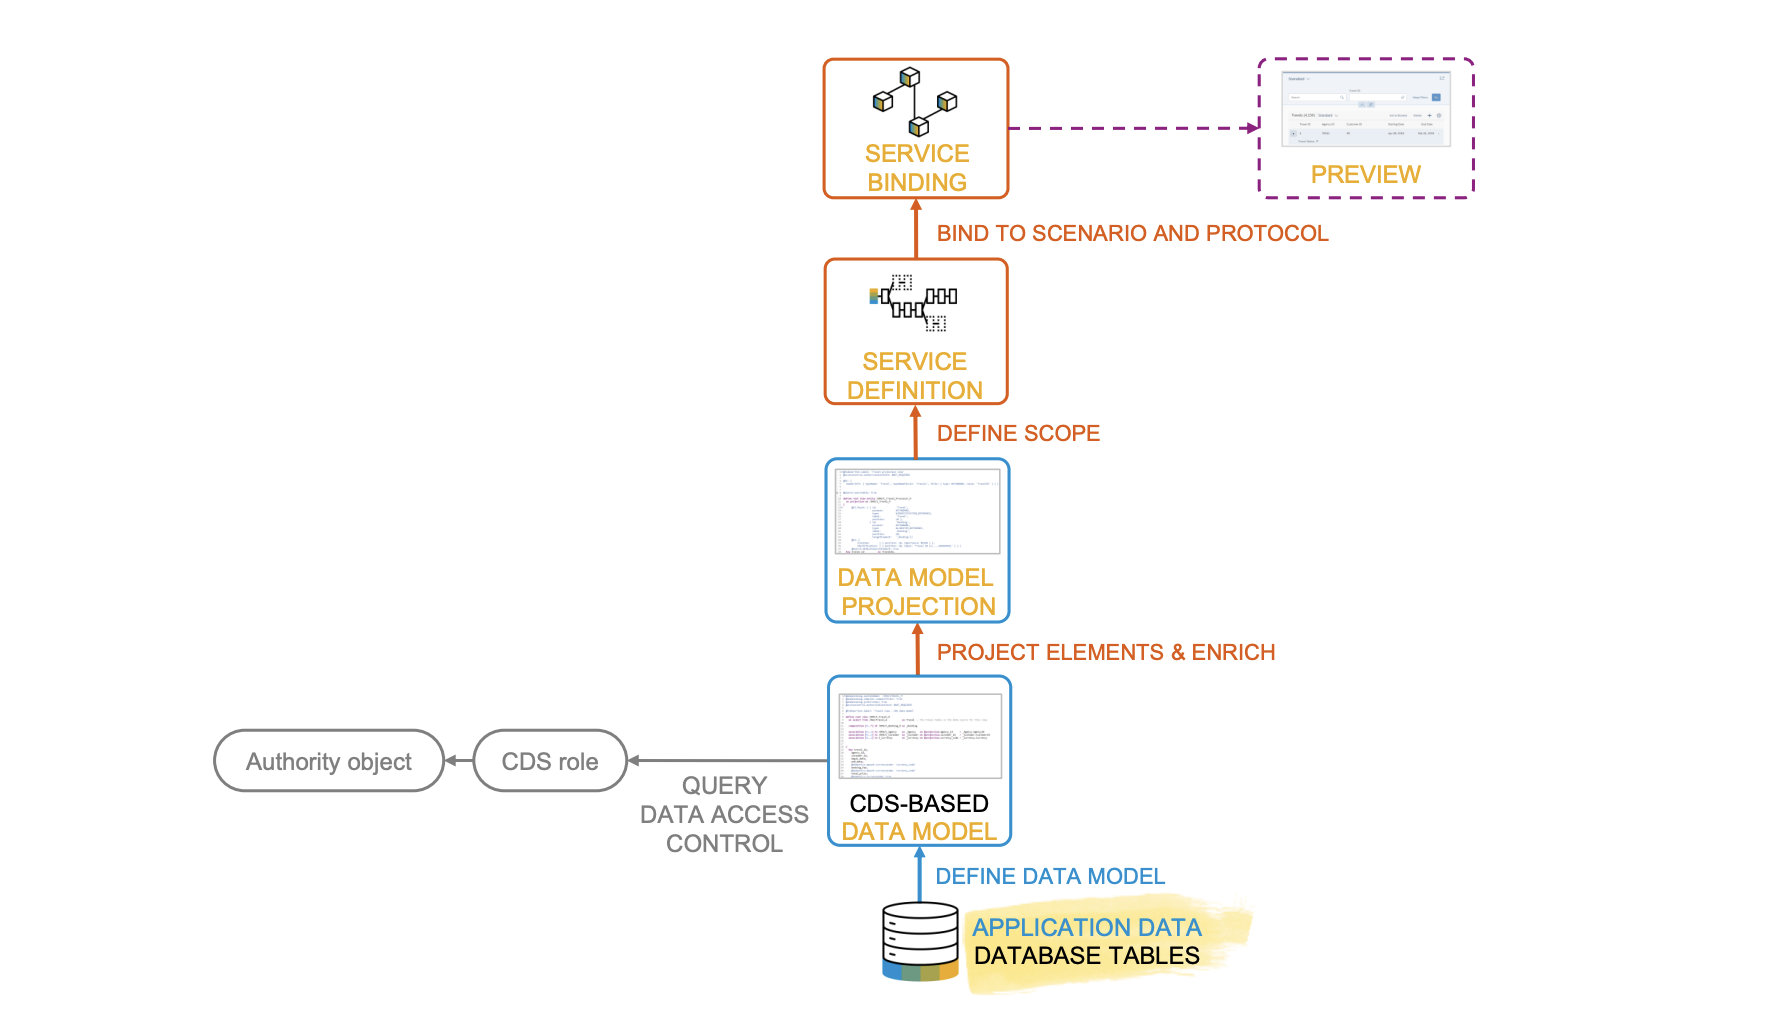
\includegraphics[width=13cm]{Figures/Screenshot-7.png}
    \caption{ABAP RAP --- Layered Architecture}
    \label{fig:rap_architecture}
\end{figure}

\begin{enumerate}
    \item \textbf{CDS View Entities} --- define the data model directly on the HANA database;
    \item \textbf{Behavior Definition (BDEF)} --- specify allowed operations (CRUD, custom actions, business logic) in ABAP;
    \item \textbf{Service Definition \& Binding} --- expose entities as \textbf{OData V4} endpoints consumable by web apps, Fiori, or mobile.
\end{enumerate}

% ─────────────────────────────────────────────
\subsection{Internship Overview}
\label{subsec:internship_overview}
% ─────────────────────────────────────────────

This section provides a structured overview of the technical internship carried out at Cognitus Corporation. It situates the project within the academic curriculum of the INPT, outlines the administrative and supervisory framework governing the internship, defines the core technical objectives of the assignment, and details the project planning, governance methodology, and technical ramp-up undertaken during this two-month immersion.

\subsubsection{Internship Framework}
\label{subsubsec:internship_framework}

The internship was conducted as the mandatory engineering initiation and technical internship (\textit{Stage INE1}) for the ASEDS program at the INPT, Rabat, under the auspices of the \textit{Agence Nationale de R\'eglementation des T\'el\'ecommunications} (ANRT). 

For me, this experience represented my very first professional internship and my initial immersion into the world of enterprise information systems and Enterprise Resource Planning (ERP). Carried out on-site (\textit{Pr\'esentiel}) at the Cognitus Global Delivery and Support Center (GDSC) in Technopark, Tangier, the internship spanned two months, from \textbf{June 15, 2026, to August 15, 2026}: eight weeks of work followed by a closure week.

All contractual, institutional, and organizational modalities were formalized in the official internship agreement (\textit{Convention de stage}). Table~\ref{tab:convention_stage} summarizes the primary administrative parameters of this engagement.

\begin{table}[H]
    \centering
    \begin{tabular}{|m{5cm}|m{9.5cm}|}
        \hline
        \textbf{Item / Field} & \textbf{Specification / Details} \\
        \hline
        \textbf{Host Enterprise} & Cognitus Corporation --- EMEA GDSC (Tangier, Morocco) \\
        \hline
        \textbf{Signatory Representative} & \textbf{Mr.\ Mohamed Reghioui} \newline \textit{Function:} General Manager EMEA \newline \textit{Email:} \href{mailto:mreghioui@cognitus.com}{mreghioui@cognitus.com} \newline \textit{Phone:} +212 (0) 661 93 99 35 \\
        \hline
        \textbf{Industrial Supervisor} & \textbf{Mr.\ Karim A\"it Alla} \newline \textit{Function:} Technical Lead \newline \textit{Email:} \href{mailto:kaitalla@cognitus.one}{kaitalla@cognitus.one} \newline \textit{Phone:} +212 (0) 611 66 58 81 \\
        \hline
        \textbf{Official Assignment Title} & \textit{D\'eveloppement des extensions pour les impl\'ementations SAP} (Development of Extensions for SAP Implementations) \\
        \hline
        \textbf{Internship Period} & June 15, 2026 -- August 15, 2026 (2 months: 8 weeks of work and a closure week) \\
        \hline
        \textbf{Working Modality} & On-site (\textit{Pr\'esentiel}) at Technopark Tangier \\
        \hline
        \textbf{Core Scope \& Missions} & 
        $\bullet$~Comprehensive understanding of enterprise ERP architecture and business workflows; \newline
        $\bullet$~Acquisition of foundational ABAP development and SAP Fiori UI concepts; \newline
        $\bullet$~Understanding, design, and construction of WRICEF objects (Workflows, Reports, Interfaces, Conversions, Enhancements, and Forms). \\
        \hline
    \end{tabular}
    \caption{Internship Agreement Administrative Specifications (\textit{Convention de stage})}
    \label{tab:convention_stage}
\end{table}

\subsubsection{Project Objectives (\textit{Objectifs du projet de stage})}
\label{subsubsec:project_objectives}

Within the broader scope of developing custom extensions for SAP implementations, the specific project assigned to me was titled: \textbf{``Design and Implementation of an Intelligent Talent Acquisition and Employee Administration System Using SAP BTP, ABAP RAP, and Artificial Intelligence''}. 

Recruitment and personnel onboarding are among the most critical operational pillars of enterprise Human Capital Management (HCM). However, traditional enterprise recruitment pipelines face significant challenges: corporate recruiters are frequently overwhelmed by high volumes of incoming applications, manual resume screening is notoriously labor-intensive and subjective, and legacy SAP GUI transaction screens are ill-suited for external candidates and modern mobile-first HR users.

To solve this dilemma, the project sought to bridge the gap between a modern, consumer-grade candidate experience and the enterprise-grade SAP back-end through six core objectives:

\begin{itemize}
    \item \textbf{SAP HCM Data Modeling via ABAP RAP:} Construct Core Data Services (CDS) view entities defining the fundamental HR data models (Organizational Units, Job Positions, Recruitment Job Offers, and Candidate Profiles) directly on the SAP HANA database layer.
    
    \item \textbf{Business Logic \& Behavior Implementation:} Define transactional behavior definitions (BDEF) in ABAP Cloud to enforce business rules, automated determinations, data validations, and state transitions across the candidate lifecycle.

    \item \textbf{Secure OData V4 API Exposure:} Expose the RAP business entities through SAP Service Definitions and Service Bindings as standard OData V4 RESTful APIs, facilitating seamless, decoupled communication with external web applications.

    \item \textbf{AI-Powered Resume Analysis \& Candidate Scoring:} Integrate an intelligent AI screening service capable of parsing semi-structured CV documents (PDF, Word, or text), extracting candidate competencies and work histories, and automatically calculating a rubric-based match score against the requirements of the job.

    \item \textbf{Decoupled External Web Portal:} Build an intuitive, responsive web portal where candidates can browse openings, submit applications, and track their progress without any direct access to the SAP backend, while recruiters review and rank the candidates in an SAP Fiori cockpit.

    \item \textbf{WRICEF Construction \& Clean Core Compliance:} Implement the required WRICEF objects (Interfaces, Reports, Enhancements) while adhering to SAP's \textit{Clean Core} principles to preserve system upgradability.
\end{itemize}

\subsubsection{Project Planning and Management}
\label{subsubsec:project_planning}

To ensure the successful delivery of an enterprise-grade cloud extension within the two-month internship timeframe, this project adopted a rigorous engineering management framework. This structure integrated an intensive preliminary training curriculum on SAP Learning, learning about HCM and S/4HANA, and an Agile development lifecycle governed by the Scrum framework.

% ══════════════════════════════════════════════
\paragraph{A. Formation et Mont\'{e}e en Comp\'{e}tences --- Technical Training \& Upskilling}
% ══════════════════════════════════════════════

Entering the SAP enterprise ecosystem required a dedicated, intensive preparation phase. The first weeks of the internship were dedicated to technical upskilling on \textbf{SAP Learning}~\cite{sap_learning}, through three official courses totalling about \textbf{41 hours} (4~h for BTP100, 17~h for S4D400, and 20~h for S4D437) with hands-on exercises in the SAP BTP ABAP Environment, alongside an exploration of SAP and Human Capital Management domain concepts:

\begin{enumerate}

    \item \textbf{Exploring SAP Business Technology Platform (BTP100)} \textit{--- Level: Beginner}

    \textit{Core Curriculum:} Covered the foundational multi-cloud architecture of SAP BTP, core infrastructure providers, security and identity provisioning, runtime environments --- Cloud Foundry, Kyma, and ABAP Cloud --- and side-by-side extension paradigms.

    \textit{Direct Project Value:} Provided the architectural blueprint to design the recruitment platform as a decoupled cloud application on SAP BTP, strictly adhering to SAP's \textbf{Clean Core} strategy by leaving standard ERP core tables untouched.

    \item \textbf{Learning Basic ABAP Programming (S4D400)} \textit{--- Level: Beginner}

    \textit{Core Curriculum:} Covered the basics of ABAP programming in the SAP BTP ABAP Environment: data types and internal tables, SQL access to database tables, modern expressions such as \texttt{VALUE}, \texttt{CORRESPONDING}, and \texttt{FILTER}, object-oriented modularization with classes and interfaces, and the Eclipse-based ABAP Development Tools.

    \textit{Direct Project Value:} Established the programmatic foundation required to write clean, type-safe business logic, custom calculations, and validation routines.

    \item \textbf{Building Transactional Apps with the ABAP RESTful Application Programming Model (S4D437)} \textit{--- Level: Advanced}

    \textit{Core Curriculum:} Delivered deep mastery of Core Data Services view entities, transactional Behavior Definitions, the RAP interaction phase and save sequence, transactional draft handling, custom business actions, determinations, validations, dynamic feature control, and publishing OData V4 Web API and UI services.

    \textit{Direct Project Value:} Formed the functional and transactional backbone of the platform, enabling robust draft state management for incomplete requisitions, fine-grained entity validation, atomic employee onboarding commits, and seamless API exposure for both the React web portal and the Python AI microservice.

    \item \textbf{SAP HCM Domain Research \& Organizational Modeling}

    In addition to technical frameworks, substantial self-directed research was conducted into standard \textbf{SAP Human Capital Management} business processes. This covered the structural relationship between \textbf{Organizational Units} and \textbf{Positions} --- enforcing vacancy states: \textit{Vacant}, \textit{Filled}, \textit{Frozen}, and budgeted compensation ceilings --- as well as classical personnel \textbf{Infotypes} for Organizational Assignment, Personal Data, Addresses, and Bank Details.

    \textit{Direct Project Value:} Enabled the reverse-engineering and modernization of standard SAP HCM structures into native CDS data models and informed the design of the atomic onboarding action that generates complete Employee Master Records.

\end{enumerate}

The completion of the courses is recorded in SAP Learning. The BTP100 and S4D400 courses award a course completion badge (Figure~\ref{fig:sap_certificate}), while S4D437 records the completion without a badge. As the learning list shows (Figure~\ref{fig:sap_learning_dashboard}), BTP100 was completed on June 15, 2026, and the S4D400 and S4D437 courses, started during the internship, were formally completed on October 11, 2026.

\begin{figure}[H]
    \centering
    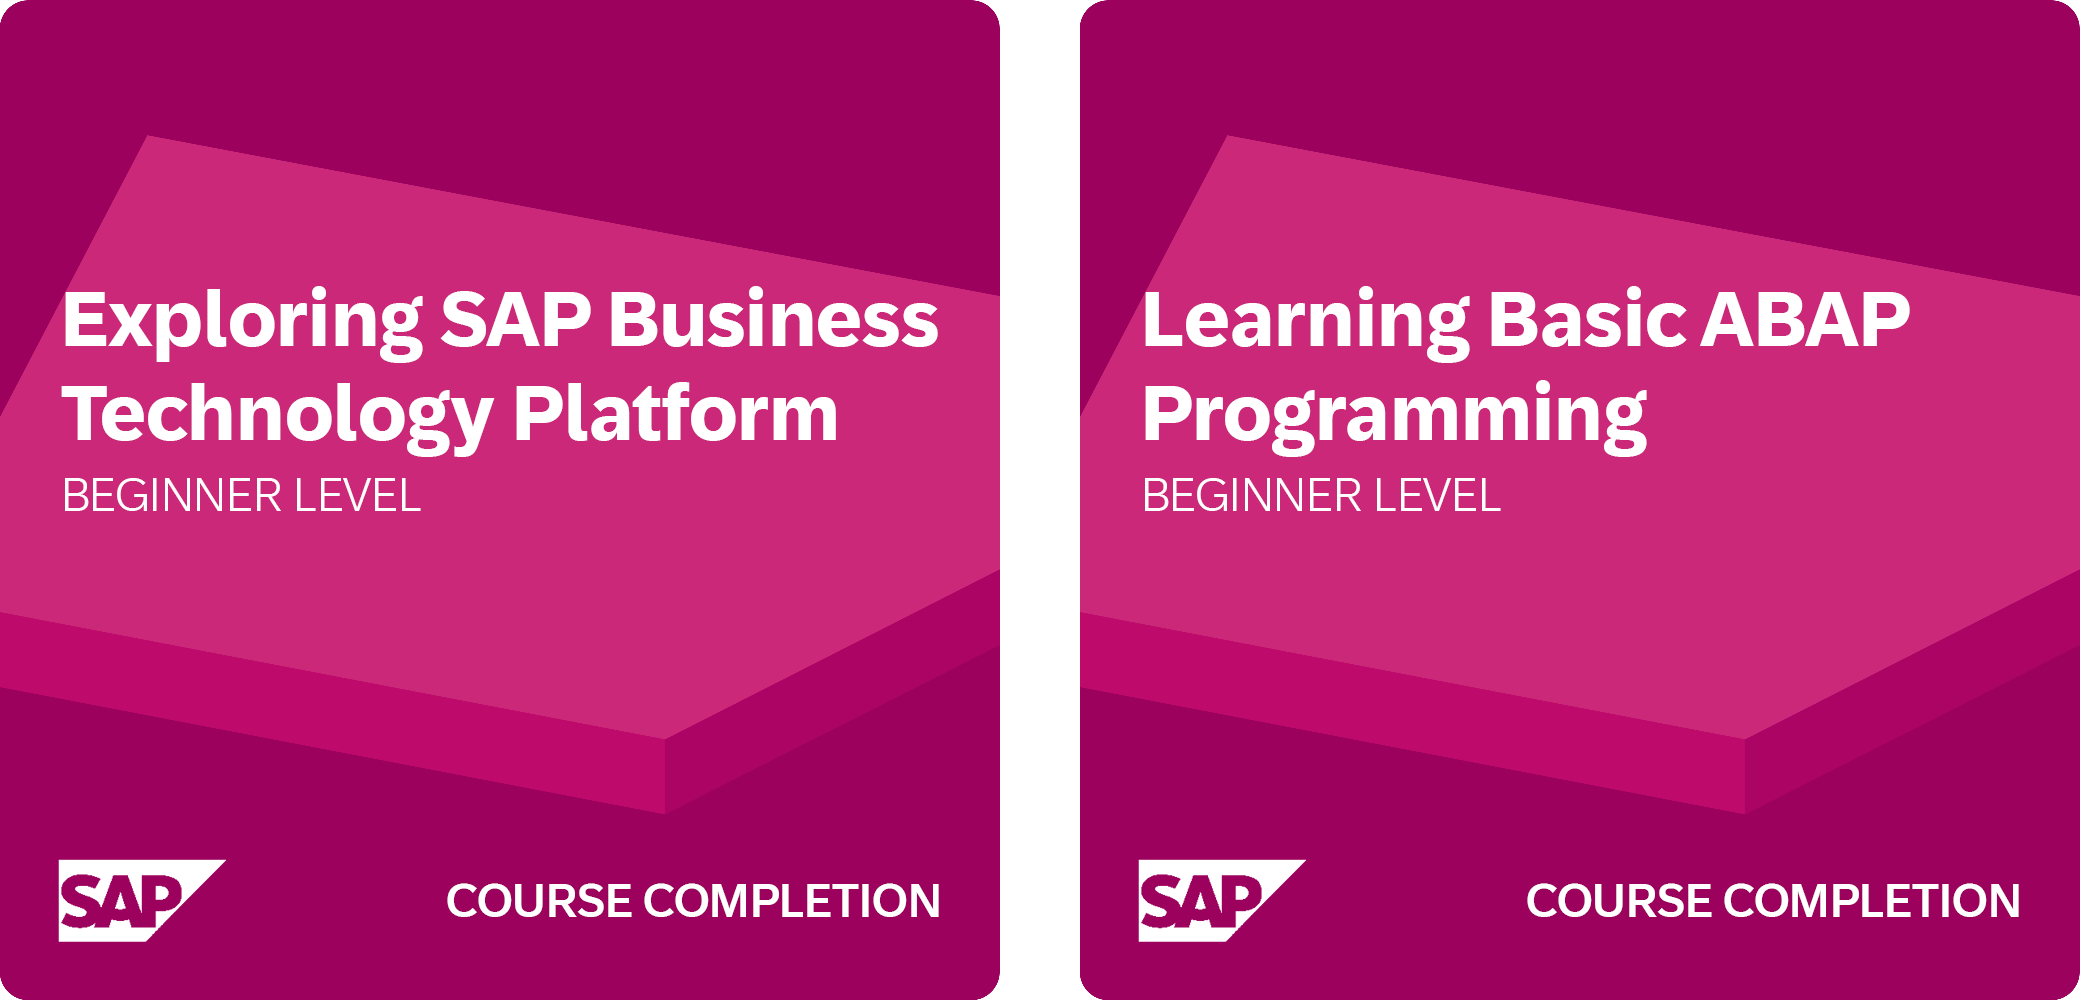
\includegraphics[width=12cm]{Figures/sap_certificate.png}
    \caption{SAP Learning --- Course Completion Badges (BTP100 and S4D400)}
    \label{fig:sap_certificate}
\end{figure}

\begin{figure}[H]
    \centering
    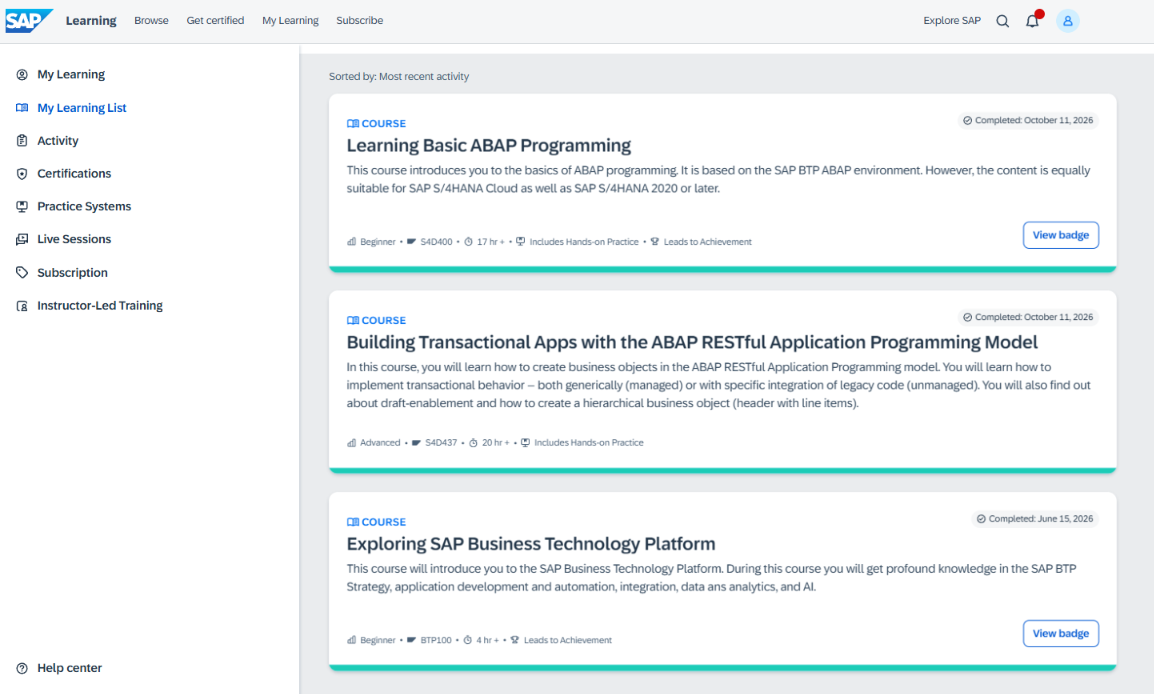
\includegraphics[width=14cm]{Figures/sap_learning_hub_dashboard.png}
    \caption{SAP Learning --- List of Completed Courses}
    \label{fig:sap_learning_dashboard}
\end{figure}

% ══════════════════════════════════════════════
\paragraph{B. Conduite de Projet --- The Scrum Framework}
% ══════════════════════════════════════════════

To manage developmental complexity and foster rapid adaptability, the project was conducted following the \textbf{Scrum Framework}~\cite{scrum_guide}, the premier agile methodology for iterative, high-value product engineering.

\textbf{Foundational Scrum Principles.} Implementing the project under Scrum best practices relied on three foundational pillars:

\begin{itemize}
    \item \textbf{Autonomous, Cross-Functional Execution} --- Rapidly pivoting technical scopes and adapting to architectural feedback through close collaboration between the intern and the industrial supervisor.
    \item \textbf{Iterative Time-Boxed Sprints} --- Organizing the development lifecycle into short, structured two-week iterations facilitating continuous integration, regular testing, and progressive feature delivery.
    \item \textbf{Product Backlog Prioritization} --- Systematically consolidating functional and non-functional requirements into a dynamic, centralized backlog that evolved as technical discoveries were made.
\end{itemize}

\begin{figure}[H]
    \centering
    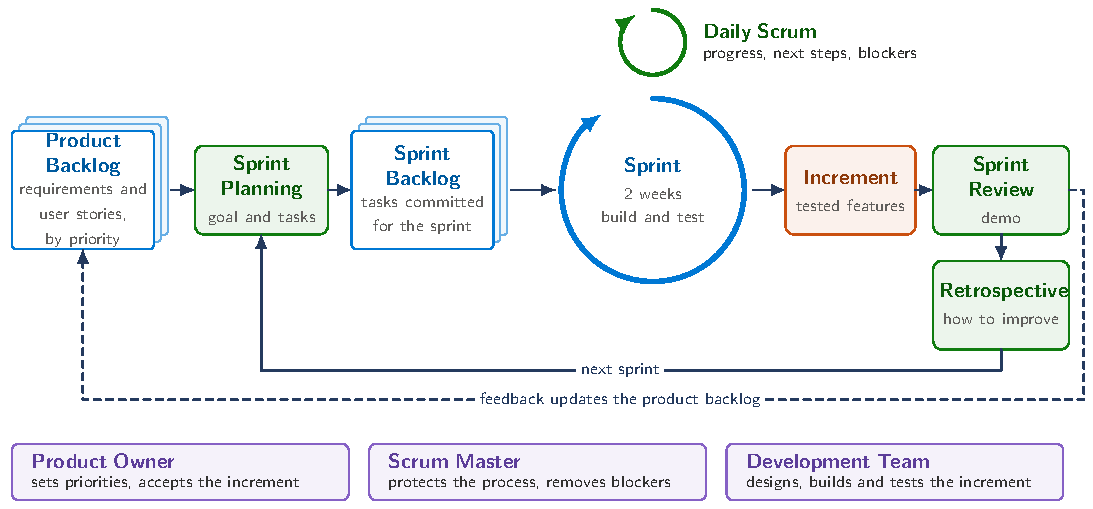
\includegraphics[width=\textwidth]{Figures/scrum_framework.pdf}
    \caption{The Scrum Framework --- Iterative Development Cycle}
    \label{fig:scrum_framework}
\end{figure}

\textbf{Scrum Roles \& Synergy.} The project established clear ownership across the three canonical Scrum roles:

\begin{itemize}
    \item \textbf{Product Owner} --- Represented by the enterprise leadership and Technical Lead, Mr.\ Karim A\"it Alla, acting as the proxy for corporate expectations, resolving requirement ambiguities, and establishing backlog priorities.
    \item \textbf{Scrum Master} --- Ensured rigorous adherence to Agile practices, monitored sprint cadence, eliminated technical roadblocks such as cloud quota allocations and API connectivity issues, and safeguarded project milestones.
    \item \textbf{Development Team} --- Executed autonomously by the intern, Mr.\ Oualid AMTOUT, assuming full technical responsibility for architectural modeling, RAP backend coding, React portal frontend engineering, AI microservice development, and testing.
\end{itemize}

\textbf{Core Scrum Ceremonies.} The iterative lifecycle was punctuated by four essential events:

\begin{itemize}
    \item \textbf{Sprint Planning} --- Conducted at the start of each iteration to decompose user stories from the Product Backlog into discrete technical tasks and commit to sprint goals.
    \item \textbf{Sprint Execution} --- The active engineering phase encompassing CDS data modeling, behavior definition programming, UI development, and API integration.
    \item \textbf{Sprint Review \& Retrospective} --- Concluding demonstrations where working increments were presented to the supervisor, followed by retrospective evaluations to optimize developmental efficiency for subsequent sprints.
    \item \textbf{Backlog Refinement} --- Continuous reassessment and estimation of upcoming user stories to adapt to emerging technical constraints.
\end{itemize}

\textbf{Sprint Plan.} The product backlog was distributed over four two-week sprints, followed by a closure week (Figure~\ref{fig:sprint_plan}). Each sprint had a goal and a set of backlog items taken from the work packages of the Software Development Plan: the first two sprints were devoted to the SAP training and the scoping of the project, the third to the specification and the data model, and the fourth to the integrated prototype, its tests, and its deployment. The backlog items were followed as task lists kept with the project documentation, and the source code was versioned on GitHub.

\begin{figure}[H]
    \centering
    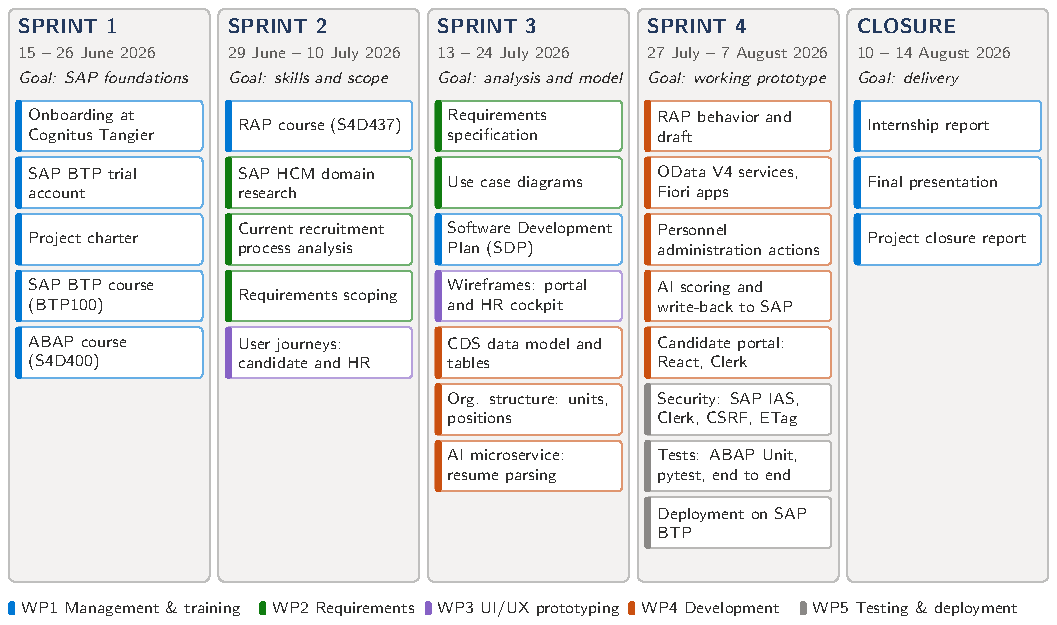
\includegraphics[width=\textwidth]{Figures/sprint_plan.pdf}
    \caption{Sprint Plan --- Product Backlog Distributed over Four Two-Week Sprints}
    \label{fig:sprint_plan}
\end{figure}

% ══════════════════════════════════════════════
\paragraph{C. Gouvernance du Projet --- Formal Governance Artifacts}
% ══════════════════════════════════════════════

Project governance and task monitoring were anchored in two formal enterprise management documents alongside a detailed Gantt schedule:

\begin{itemize}

    \item \textbf{Project Charter:} This document formalizes the context, goal, and objectives of the project, its scope (inclusions and exclusions), the chosen delivery strategy, the stakeholder analysis, the main risks with their mitigation, a preliminary budget and schedule, and the value expected from the solution. Figure~\ref{fig:charte_projet} shows its delivery strategy section, which compares an internal, an external, and a joint delivery.

    \begin{figure}[H]
        \centering
        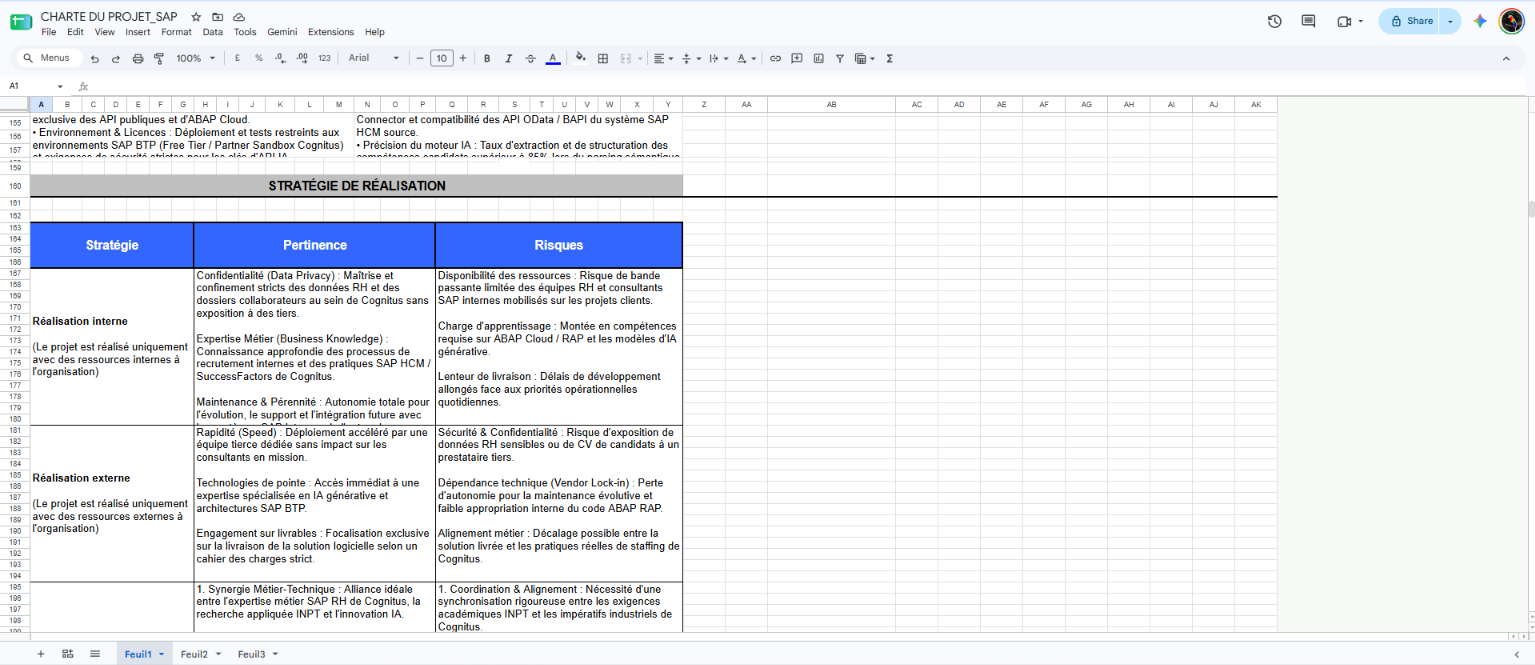
\includegraphics[width=\textwidth]{Figures/charte_projet.png}
        \caption{Project Charter --- Delivery Strategy Section}
        \label{fig:charte_projet}
    \end{figure}

    \item \textbf{Software Development Plan:} The SDP is the operational plan of the project. Its work breakdown structure organizes the work into \textbf{five work packages} (Figure~\ref{fig:sdp_document}):

    \begin{enumerate}
        \item \textbf{WP1 --- Project Management and Training:} project charter, development plan, SAP BTP trial account, SAP courses, internship report, and closure report.
        \item \textbf{WP2 --- Requirements \& Specifications Analysis:} analysis of the current process, SAP HCM recruitment and personnel administration workflows, functional and non-functional requirements, use cases, comparison of language models, and conceptual data model.
        \item \textbf{WP3 --- UI/UX Prototyping:} user journeys, wireframes of the candidate portal and of the HR cockpit, application and onboarding forms, and visual style.
        \item \textbf{WP4 --- Backend \& Frontend Development:} database tables, CDS views, behavior definitions and business objects, OData V4 services, the React candidate portal, and the FastAPI AI microservice.
        \item \textbf{WP5 --- Testing \& Deployment:} unit and integration tests, tests of the recruitment pipeline and of the onboarding, edge cases, end-to-end tests, and deployment on SAP BTP.
    \end{enumerate}

    This report follows the same structure: the analysis of Chapter~\ref{chap:analysis_specifications} and the design of Chapter~\ref{chap:solution_design} cover WP2 and WP3, and the realization and tests of Chapter~\ref{chap:implementation} cover WP4 and WP5.

    \begin{figure}[H]
        \centering
        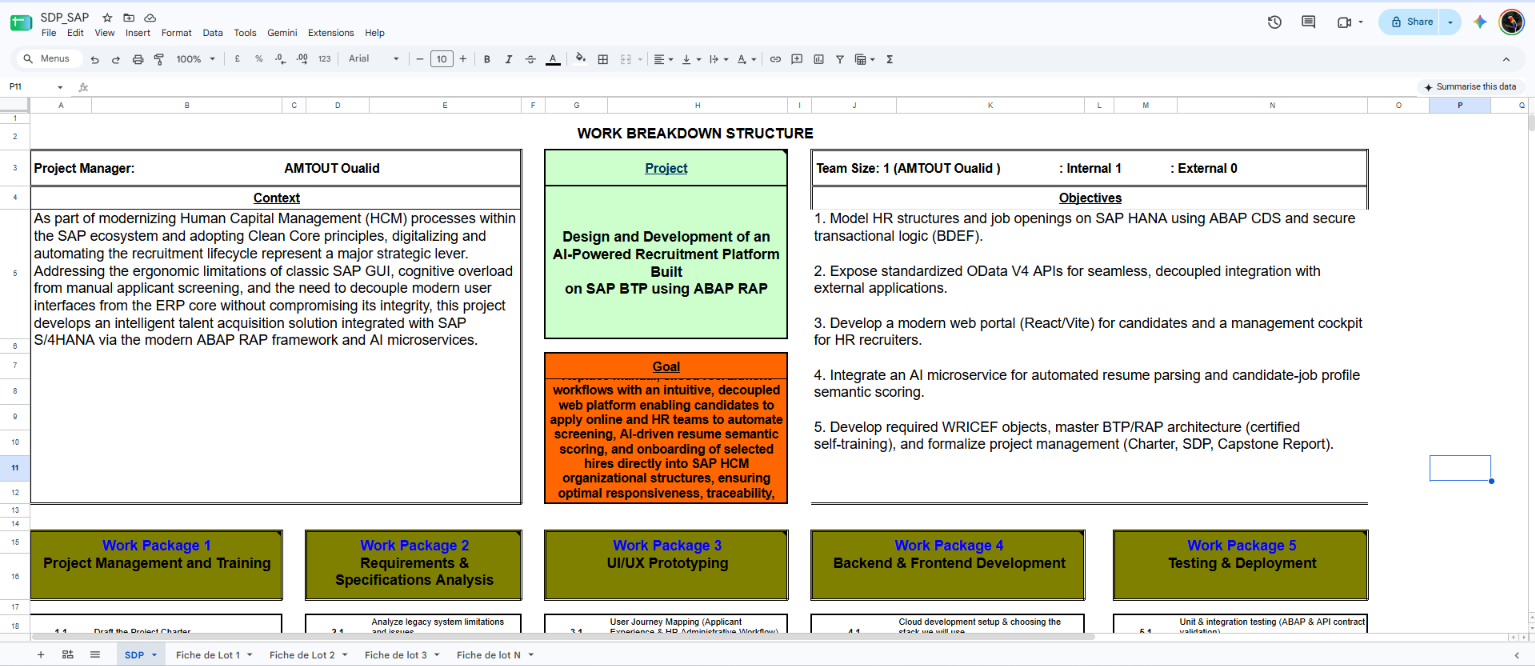
\includegraphics[width=\textwidth]{Figures/sdp_document.png}
        \caption{Software Development Plan --- Work Breakdown Structure}
        \label{fig:sdp_document}
    \end{figure}

\end{itemize}

The main risks identified in the project charter, with their assessment and the measures taken to reduce them, are summarized in Table~\ref{tab:risk_matrix}.

\begin{table}[H]
\centering
\caption{Main Project Risks and Mitigation Measures}
\label{tab:risk_matrix}
\renewcommand{\arraystretch}{1.3}
\setlength{\tabcolsep}{4pt}
\footnotesize
\begin{tabular}{|>{\raggedright\arraybackslash}p{4.0cm}|>{\raggedright\arraybackslash}p{1.3cm}|>{\raggedright\arraybackslash}p{2.0cm}|>{\raggedright\arraybackslash}p{1.85cm}|>{\raggedright\arraybackslash}p{2.35cm}|>{\raggedright\arraybackslash}p{5.25cm}|}
\hline
\textbf{Risk} & \textbf{Impact} & \textbf{Probability} & \textbf{Criticality} & \textbf{Category} & \textbf{Mitigation} \\
\hline
R1. Integration of the three components: OData V4 calls from the React portal (CSRF, ETag, CORS, sessions of the trial account) and write-back of the AI score & High & Medium & High & Technical & Dedicated RAP actions (\texttt{applyToJob}, \texttt{setAIEvaluation}), development proxy for the portal, and early end-to-end tests. \\
\hline
R2. Quality of the AI evaluation: incomplete parsing of heterogeneous resumes or wrong assessment of the skills & Medium & Medium & Medium & Functional, AI & Normalized prompts, strict JSON output, score computed in Python, human decision required, and tests on fictitious resumes of different levels. \\
\hline
R3. Confidentiality: exposure of the personal data of candidates or employees & Critical & Low & High & Security, legal & Separate authentication (SAP IAS for HR, Clerk for candidates), HTTPS, fictitious test resumes, and an AI microservice without database. \\
\hline
R4. User adoption: reluctance toward new screens and algorithmic suggestions & Medium & Low & Low & Organizational & Standard SAP Fiori Elements interfaces, screen mockups, and regular demonstrations. \\
\hline
R5. Trial account and schedule: session expiry, limits of the SAP BTP trial account, and risk of exceeding the planned weeks & High & Low & Medium & Planning, infrastructure & Scrum with two-week sprints, prioritized minimum viable product, and regular backup of the code with abapGit and GitHub. \\
\hline
\end{tabular}
\end{table}

% ══════════════════════════════════════════════
\paragraph{D. Planning d'Ex\'{e}cution --- Implementation Schedule \& Gantt Diagram}
% ══════════════════════════════════════════════

The eight weeks of work were organized in four phases, followed by a closure week, as summarized in Table~\ref{tab:implementation_phases}.

\begin{table}[H]
\centering
\caption{Implementation Schedule --- Phases, Timeframes, and Key Milestones}
\label{tab:implementation_phases}
\renewcommand{\arraystretch}{1.4}
\small
\begin{tabular}{|>{\raggedright\arraybackslash}p{2.6cm}|>{\raggedright\arraybackslash}p{2.2cm}|>{\raggedright\arraybackslash}p{9.2cm}|}
\hline
\textbf{Phase} & \textbf{Timeframe} & \textbf{Focus Area \& Key Milestones} \\
\hline
Phase 1: Onboarding \& Training & Weeks 1--4 & Team integration at Technopark Tangier, SAP Learning courses (BTP100, S4D400, S4D437), project charter, and initial requirement scoping. \\
\hline
Phase 2: Analysis \& Data Modeling & Weeks 5--6 & Software Development Plan, requirements and UML use cases, CDS data model, and organizational structure modeling. \\
\hline
Phase 3: Development \& Integration & Weeks 6--7 & RAP behavior definitions, draft handling, OData V4 services, Fiori Elements applications, FastAPI AI microservice, and React candidate portal. \\
\hline
Phase 4: Testing \& Finalization & Week 8 & Unit and end-to-end tests, feature control validation, deployment on SAP BTP, and technical documentation. \\
\hline
Closure & Week 9 & Internship report, presentation, and project closure report. \\
\hline
\end{tabular}
\end{table}

The detailed schedule, with its tasks, dependencies, and milestones, was modeled with \textbf{GanttProject}~\cite{ganttproject}, as illustrated in Figure~\ref{fig:gantt_diagram}.

\begin{figure}[H]
    \centering
    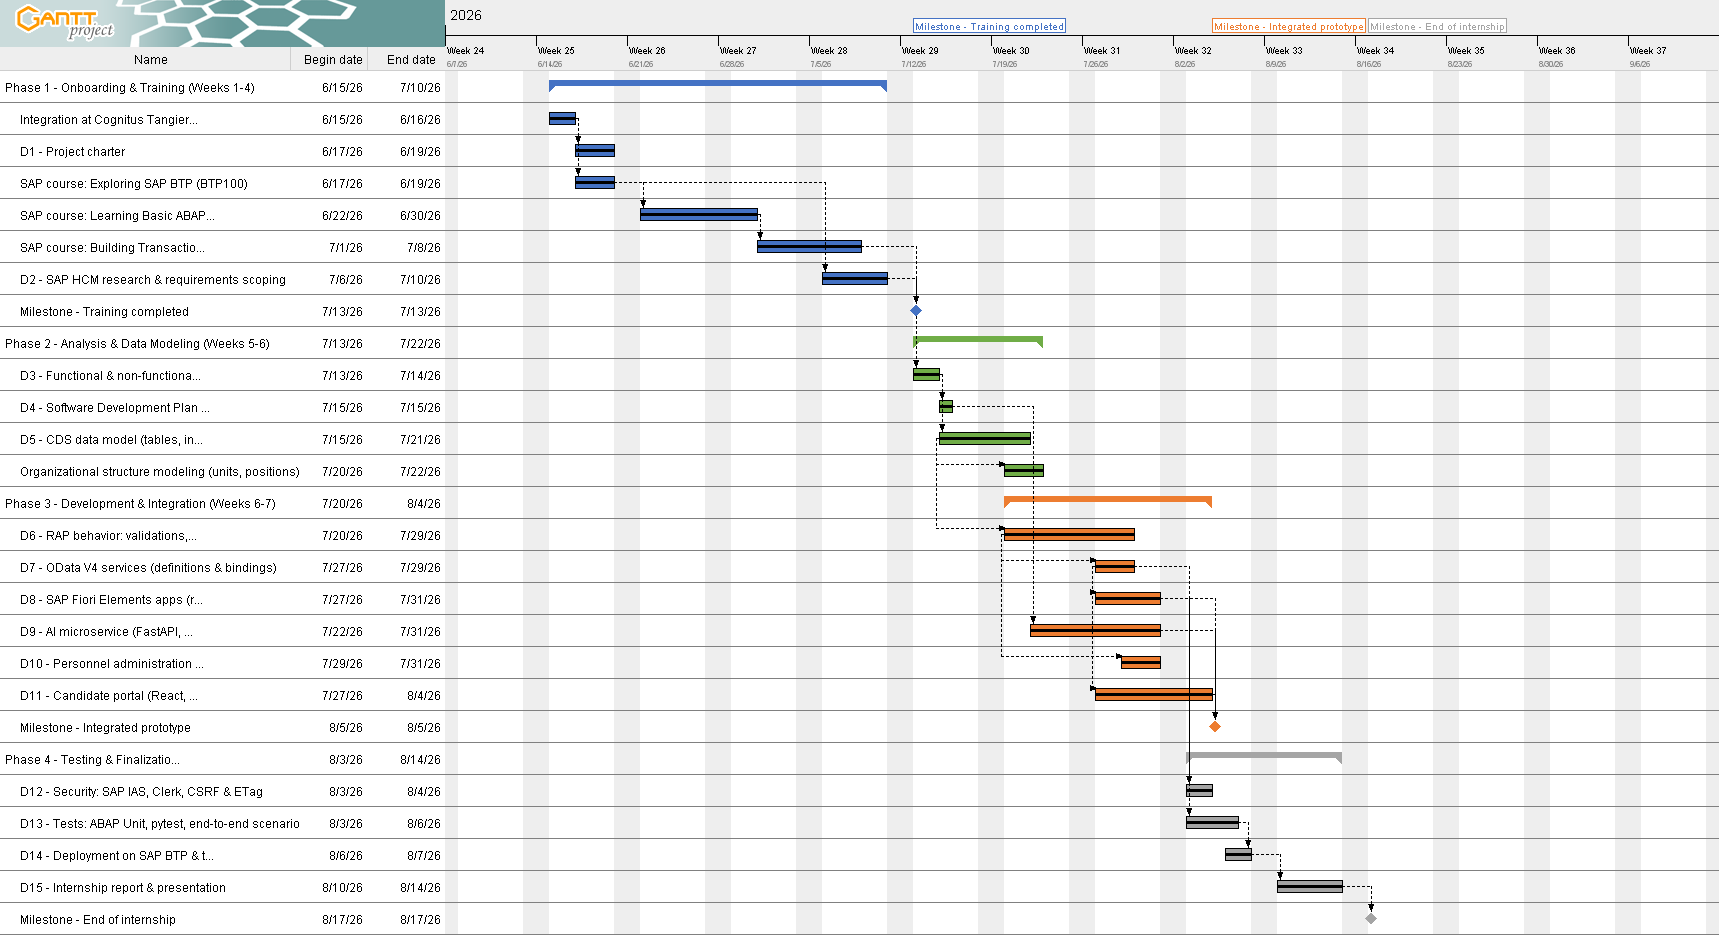
\includegraphics[width=\textwidth]{Figures/Gantt_Diagram.png}
    \caption{Project Planning --- Detailed Gantt Diagram}
    \label{fig:gantt_diagram}
\end{figure}

\newpage

% ─────────────────────────────────────────────
\section*{Conclusion}
\addcontentsline{toc}{section}{Conclusion}
% ─────────────────────────────────────────────

This chapter introduced Cognitus Corporation, a global SAP Gold Partner now part of IBM, and its Tangier Global Delivery and Support Center where this work was carried out. We examined the company's core business areas, key industries, and notable client portfolio, then established the conceptual foundations of ERP systems and the modern SAP technology stack underpinning this project. Finally, we detailed the institutional framework, technical objectives, training curriculum, Scrum-based project governance, and structured implementation schedule that guided the two-month internship. The following chapter presents the project context and objectives in greater detail.


\chapter{Project Context and Objectives}
\label{chap:project_context_objectives}

% ─────────────────────────────────────────────
\section*{Introduction}
\addcontentsline{toc}{section}{Introduction}
% ─────────────────────────────────────────────

This chapter delineates the foundational context and strategic perimeter of the project. It begins by establishing the general context of enterprise software modernization, examining how digital transformation and cloud architectures intersect with corporate talent acquisition. Next, it details the core operational and architectural problem statement that motivated this work, analyzing the systemic bottlenecks of manual screening, rigid legacy ERP workflows, semantic keyword limitations, and master data isolation. Finally, it articulates the primary project objectives guiding the design and development of the proposed cloud-native, AI-powered recruitment platform built on SAP BTP using ABAP RAP.

\newpage

% ─────────────────────────────────────────────
\section{General Project}
\label{sec:general_project}
% ─────────────────────────────────────────────

\subsection{General Context}
\label{subsec:general_context}

Enterprise Resource Planning (ERP) systems constitute the central digital backbone of modern organizations, orchestrating mission-critical financial and human capital processes. However, while core transactional systems have largely transitioned to scalable cloud architectures, corporate recruitment workflows often remain fragmented, relying on manual screening methods, disconnected point solutions, and legacy procedures that introduce substantial administrative overhead and hiring latency.

Building upon intensive technical upskilling on SAP Business Technology Platform (SAP BTP), ABAP Cloud, and the ABAP RESTful Application Programming Model (RAP), this project addresses these operational hurdles. It aims to design and implement an AI-powered talent acquisition platform that unifies modern candidate self-service with robust enterprise SAP HCM governance, while strictly adhering to SAP's Clean Core extensibility principles.

\subsection{Problem Statement}
\label{subsec:problem_statement}

Despite the strategic importance of talent acquisition, enterprise recruitment workflows face several operational and architectural bottlenecks that can be synthesized as follows:

\begin{itemize}
    \item \textbf{Manual Screening Overload and Latency:} Inundated by large application volumes, recruiters face severe cognitive fatigue from manual resume review, substantially inflating time-to-hire and introducing subjective evaluation biases.

    \item \textbf{Workflow Rigidity and Poor Ergonomics:} Legacy ERP systems feature complex transactional interfaces designed strictly for back-office administration, lacking candidate self-service portals and agile pipeline tracking workflows.

    \item \textbf{Semantic Inadequacy in Traditional ATS:} Conventional keyword-matching tools lack semantic reasoning, frequently rejecting qualified applicants due to vocabulary mismatches while rewarding candidates who practice artificial keyword stuffing.

    \item \textbf{Enterprise ERP Isolation and Manual Re-entry:} Disconnected third-party recruitment tools force manual transcription of hired candidate data into SAP HCM records, creating data discrepancies, operational delays, and Clean Core upgrade risks.
\end{itemize}

\subsection{Project Objectives}
\label{subsec:project_objectives}

In direct response to the operational bottlenecks and technological limitations identified in the problem statement, this project aims to design and implement an enterprise-grade, cloud-native recruitment and talent acquisition platform. The primary objectives guiding the realization of this system are defined as follows:

\begin{itemize}
    \item \textbf{Needs Analysis and Technology Selection}
    
    Conduct a rigorous requirements analysis across the recruitment and onboarding lifecycle, evaluating and selecting an optimal technology stack capable of supporting enterprise scalability, multi-cloud flexibility, and intelligent automation.

    \item \textbf{Native SAP Ecosystem and ERP Integrability}
    
    Build the platform natively within the SAP cloud ecosystem (SAP BTP) using modern ABAP Cloud, ensuring seamless integration with existing enterprise ERP infrastructure while strictly adhering to Clean Core principles.

    \item \textbf{Organizational Structure and Job Offer Governance}
    
    Enable HR administrators to model organizational units, create and allocate positions linked to those units, define and publish job offers, and oversee the full recruitment pipeline directly anchored to organizational vacancies.

    \item \textbf{AI Resume Analysis Engine}

    Develop a multi-stage AI microservice that uses a large language model to parse resumes into structured profiles, enrich them with the candidate's GitHub projects, and score each candidate against the job offer with explainable results.

    \item \textbf{Comprehensive Quality Assurance, Verification, and Cloud Deployment}

    Test the backend business logic, the AI microservice, and the complete recruitment process at several levels (unit tests, an end-to-end scenario, an evaluation of the AI engine, and measurements of security and response times) to verify the reliability and data integrity of the platform deployed on SAP BTP.
\end{itemize}
\newpage
% ─────────────────────────────────────────────
\section*{Conclusion}
\addcontentsline{toc}{section}{Conclusion}
% ─────────────────────────────────────────────

This chapter has established the foundational framework of the project, analyzing the general context of enterprise ERP and recruitment modernization. It has articulated the core problem statement, highlighting the operational bottlenecks, user experience deficiencies, semantic limitations of keyword ATS, and architectural disconnects with central HR systems. In response to these challenges, the chapter defined the strategic objectives of the project, spanning technology selection, native SAP BTP Clean Core integration, organizational structure modeling, AI resume analysis, and rigorous end-to-end verification. Having delineated the contextual perimeter and goals of the initiative, the next chapter will present the comprehensive analysis and detailed specifications of the proposed platform.


\chapter{Analysis and Specifications}
\label{chap:analysis_specifications}

% ─────────────────────────────────────────────
\section*{Introduction}
\addcontentsline{toc}{section}{Introduction}
% ─────────────────────────────────────────────

This chapter evaluates the current enterprise recruitment methods, identifies their systemic limitations, and presents the distinctive advantages of our proposed platform. It then formally specifies the functional and non-functional requirements alongside global use case modeling.

\newpage

% ═══════════════════════════════════════════════
\section{Existing System Study}
\label{sec:existing_system_study}
% ═══════════════════════════════════════════════

% ──────────────────────────────────────────────
\subsection{Current Recruitment Methods}
\label{subsec:current_methods}
% ──────────────────────────────────────────────

Enterprise recruitment today relies on three dominant technology models, each with distinct operational characteristics:

\begin{itemize}
    \item \textbf{Commercial SaaS ATS Platforms} --- Workday Recruiting, Oracle Taleo, Greenhouse, iCIMS Talent Cloud
    \item \textbf{Legacy On-Premise ERP Modules} --- SAP HCM Personnel Administration, SAP Recruitment, SAP Organizational Management via SAP GUI
    \item \textbf{Hybrid Manual Workflows} --- Spreadsheet-based tracking, email-driven communication, disconnected document storage
\end{itemize}

While these approaches offer partial solutions --- SaaS platforms provide modern candidate portals and pipeline visualization, ERP modules ensure data consistency within the corporate system, and manual workflows offer flexibility --- they share a common set of structural deficiencies. SaaS platforms operate in isolation from the enterprise ERP core, forcing HR staff to manually re-enter candidate data after hiring, a slow and error-prone step on records that later feed payroll. Legacy SAP GUI screens are inaccessible to external candidates and offer \textbf{no self-service}. Resume screening relies either on manual reading or on rigid keyword matching, which can reject qualified candidates whose resumes do not use the expected words. Furthermore, any customization of on-premise ERP recruitment workflows requires invasive core modifications that violate SAP's Clean Core paradigm and generate significant technical debt.

% ──────────────────────────────────────────────
\subsection{Particularities of Our Solution}
\label{subsec:solution_particularities}
% ──────────────────────────────────────────────

Our platform addresses every limitation identified above through three architectural pillars:

\textbf{Native SAP BTP Clean Core Integration.} Upon HR approval, a single RAP action creates the employee master record and its child records from the verified onboarding data, in less than half a second in our measurements and without any manual re-entry. Built as a side-by-side extension on SAP BTP using ABAP Cloud and SAP HANA Cloud, the architecture leaves the standard ERP objects untouched, which keeps the core upgradable (Clean Core).

\textbf{AI-Assisted Resume Screening.} A Python microservice uses a large language model (GPT-4o-mini) to parse each resume into a structured profile, enrich it with the candidate's GitHub projects, and score it against the rubric of the role and the requirements of the job offer, with evidence for each criterion. The final score is computed deterministically in Python. The evaluation runs in the background, takes about half a minute to a minute per resume, and costs about 0.003~USD. Transparent per-criterion scores with natural-language justifications keep the recruiter in control of the decision.

\textbf{Dual Modern User Experience.} A responsive React/Vite candidate portal enables job discovery, one-click application, real-time pipeline tracking, and onboarding self-service. An enterprise SAP Fiori Elements cockpit equips recruiters with draft handling, configurable pipelines, and one-click stage progression.

\subsection{Comparative Synthesis}
\label{subsec:comparative_synthesis}

\begin{table}[H]
\centering
\caption{Comparative Analysis --- Current Methods vs.\ Our Proposed Solution}
\label{tab:comparative_synthesis}
\renewcommand{\arraystretch}{1.4}
\small
\begin{tabular}{|>{\raggedright\arraybackslash}p{3.5cm}|>{\raggedright\arraybackslash}p{3cm}|>{\raggedright\arraybackslash}p{3cm}|>{\raggedright\arraybackslash}p{4.2cm}|}
\hline
\textbf{Dimension} & \textbf{SaaS ATS} & \textbf{Legacy SAP GUI} & \textbf{Our Solution} \\
\hline
ERP Data Integration & Isolated silo, manual re-entry & Native but internal only & \textbf{Native \& decoupled via SAP BTP} \\
\hline
Employee Creation & Manual re-entry after hiring & Manual admin action & \textbf{Automatic, about 0.4~s, no re-entry} \\
\hline
Candidate Self-Service & Web portal available & Non-existent & \textbf{Responsive React portal} \\
\hline
Resume Screening & Keyword matching & Manual reading & \textbf{AI rubric scoring with evidence, in the background} \\
\hline
Recruiter Interface & Modern dashboard & Archaic GUI screens & \textbf{SAP Fiori cockpit with drafts} \\
\hline
Clean Core Safety & External subscription & Core modifications & \textbf{No SAP standard object modified} \\
\hline
\end{tabular}
\end{table}

\newpage

% ═══════════════════════════════════════════════
\section{Requirements Identification and Analysis}
\label{sec:requirements_analysis}
% ═══════════════════════════════════════════════

% ──────────────────────────────────────────────
\subsection{Feature Identification and System Actors}
\label{subsec:feature_identification}
% ──────────────────────────────────────────────

The system engages external applicants through a public web portal and empowers internal HR personnel via an enterprise cockpit on SAP BTP. The actors are organized into two categories:

\subsubsection{Primary Actors}

\begin{enumerate}
    \item \textbf{External Candidate} --- Prospective applicants who discover job openings, submit multi-format applications, track pipeline progress, and complete the digital onboarding dossier upon selection.

    \item \textbf{HR Recruiter} --- Operational HR professionals who create and publish job requisitions, configure pipeline stages, consult AI evaluations, advance or reject applicants, and curate the Talent Pool.

    \item \textbf{HR Administrator} --- Senior HR personnel who manage the organizational hierarchy and positions, audit onboarding submissions, and execute the atomic action generating SAP Employee Master Records.
\end{enumerate}

\subsubsection{Secondary Actors}

\begin{enumerate}
    \item \textbf{AI Evaluation Microservice} --- Background service that reads resumes, extracts structured data, computes rubric-based match scores, and returns explainable evaluations that are stored with the application in SAP.

    \item \textbf{SAP ERP Backbone} --- Central system of record that maintains employee master data, enforces organizational structures, and guarantees transactional integrity via OData V4 services.
\end{enumerate}

% ──────────────────────────────────────────────
\subsection{Functional Requirements}
\label{subsec:functional_requirements}
% ──────────────────────────────────────────────

The functional requirements define the core capabilities delivered by the platform, leveraging the SAP RAP managed scenario for transactional governance and draft handling:

\begin{enumerate}

    \item \textbf{Organizational Structure and Position Management}
    \begin{itemize}
        \item \textbf{Unit Administration:} HR administrators create, update, and organize hierarchical organizational units with departmental relationships.
        \item \textbf{Position Allocation:} Positions are anchored to organizational units with budgeted salary ranges and occupancy states --- Vacant, Filled, or Frozen.
        \item \textbf{Position Validation:} Job offers can only be assigned to authorized positions currently in Vacant status.
    \end{itemize}

    \item \textbf{Job Requisition and Pipeline Lifecycle}
    \begin{itemize}
        \item \textbf{Draft Handling:} Recruiters prepare and edit job requisitions in draft mode; unfinished work is saved automatically without affecting active records.
        \item \textbf{Pipeline Stages:} Recruiters configure multi-step pipelines per job offer with customizable sequence order.
        \item \textbf{Requisition Actions:} Dedicated actions publish, close, or reopen job requisitions.
        \item \textbf{Feature Control:} Dynamic field editability and action availability adapt to the current requisition status.
    \end{itemize}

    \item \textbf{Public Candidate Portal}
    \begin{itemize}
        \item \textbf{Job Discovery:} Candidates browse published offers, filter opportunities, and view role specifications.
        \item \textbf{Application Submission:} Candidates submit applications with contact details and upload resumes in PDF, Word, or plain text.
        \item \textbf{Tracking and Self-Service:} Candidates track real-time pipeline progression or withdraw their application.
    \end{itemize}

    \item \textbf{AI Resume Analysis}
    \begin{itemize}
        \item \textbf{Document Parsing:} The AI pipeline normalizes heterogeneous resumes (PDF, DOCX, TXT) and extracts structured candidate data.
        \item \textbf{Rubric Scoring:} A matching score is computed between the candidate's experience and the requirements of the role and of the job offer, with key strengths and areas for improvement.
        \item \textbf{Evaluation Integration:} Scores and evaluation dossiers are transmitted to the SAP backend to rank applicants.
    \end{itemize}

    \item \textbf{Candidate Evaluation and Stage Progression}
    \begin{itemize}
        \item \textbf{Review Cockpit:} Recruiters view AI-generated scores and manage applicant progression across pipeline stages.
        \item \textbf{Stage Actions:} Recruiters advance, put on hold, reject, or accept candidates, record HR notes, and send e-mails to the candidates.
    \end{itemize}

    \item \textbf{Automated Onboarding and Employee Creation}
    \begin{itemize}
        \item \textbf{Onboarding Wizard:} Accepted candidates complete a secure form with personal, banking, and emergency contact information.
        \item \textbf{Atomic Employee Creation:} HR administrators trigger an approval action that generates the Employee Master Record and updates the position status from Vacant to Filled in a single transaction.
    \end{itemize}

    \item \textbf{Employee Lifecycle and Talent Pool}
    \begin{itemize}
        \item \textbf{Personnel Administration:} HR personnel update employee details, execute promotions, or reassign employees across units.
        \item \textbf{Talent Pool:} Non-selected candidates are cataloged in a centralized pool for future re-engagement.
    \end{itemize}

\end{enumerate}

% ──────────────────────────────────────────────
\subsection{Non-Functional Requirements}
\label{subsec:nonfunctional_requirements}
% ──────────────────────────────────────────────
Beyond its functional scope, the platform must satisfy the following quality requirements:
\begin{itemize}
    \item \textbf{Security:} CSRF token validation, instance-level authorization controls, and dynamic feature toggling based on entity state.

    \item \textbf{Performance:} SAP HANA Cloud in-memory processing keeps the SAP operations under one second, and the AI evaluation runs asynchronously, so that users never wait for it.

    \item \textbf{Maintainability:} Clean Core compliance (ABAP for Cloud Development, released APIs only, behavior definitions in strict mode 2) and clear RAP layer separation.

    \item \textbf{Availability:} Transactional draft mechanism preserves in-progress data across session interruptions.

    \item \textbf{Interoperability:} Standardized OData V4 service contracts enable consumption by SAP Fiori, React, and Python clients.
\end{itemize}

% ──────────────────────────────────────────────
\subsection{Global Use Case Diagram}
\label{subsec:use_case_diagram}
% ──────────────────────────────────────────────

\begin{figure}[H]
    \centering
    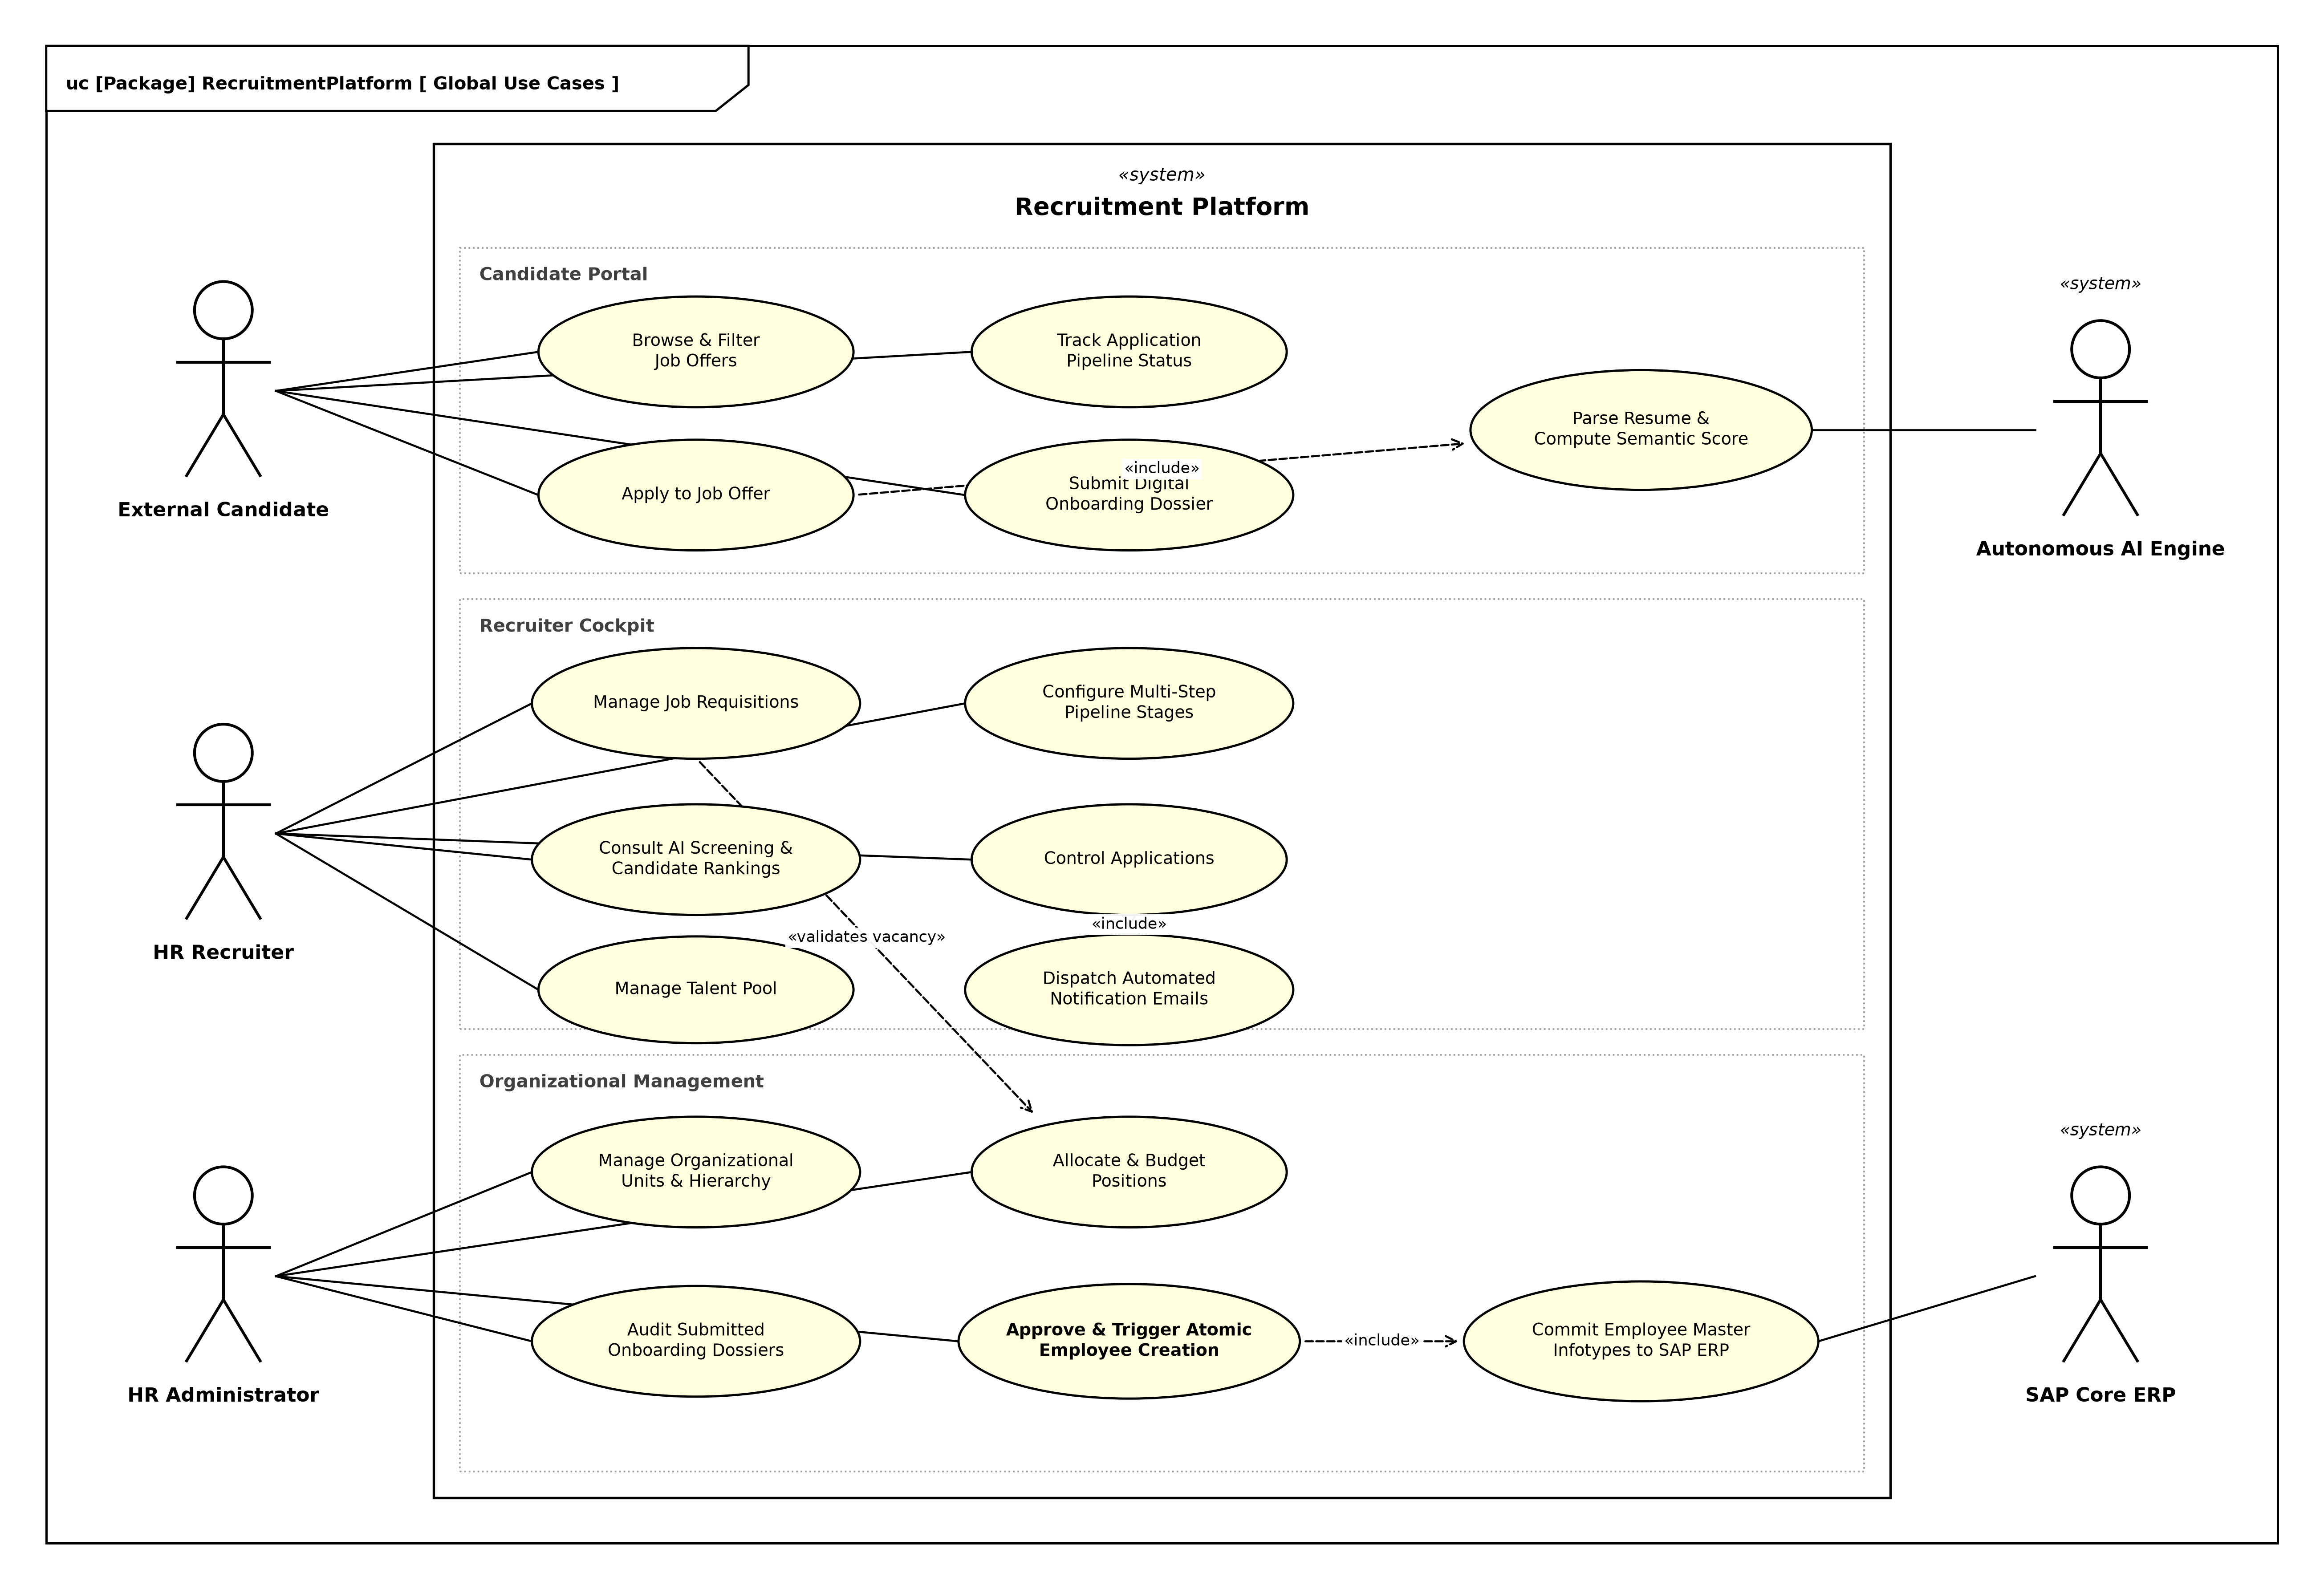
\includegraphics[width=15cm]{Figures/use_case_diagram.png}
    \caption{Global System Use Case Diagram}
    \label{fig:use_case_diagram}
\end{figure}

\subsubsection{User Stories}

\textbf{External Candidate:} Discovers a published job offer $\rightarrow$ submits application with resume $\rightarrow$ tracks real-time pipeline progression $\rightarrow$ completes onboarding dossier upon acceptance.

\textbf{HR Recruiter:} Creates job requisition in draft mode $\rightarrow$ configures pipeline stages and publishes $\rightarrow$ consults AI-generated candidate rankings $\rightarrow$ advances or rejects applicants through each stage.

\textbf{HR Administrator:} Models organizational hierarchy and creates vacant positions $\rightarrow$ audits submitted onboarding dossiers $\rightarrow$ triggers atomic employee creation $\rightarrow$ position status updates from Vacant to Filled.

% ─────────────────────────────────────────────
\section*{Conclusion}
\addcontentsline{toc}{section}{Conclusion}
% ─────────────────────────────────────────────

This chapter analyzed the existing recruitment landscape, compared it with our platform in a comparative synthesis, and established a complete specification of functional and non-functional requirements with global use case modeling. The next chapter details the architecture and the design of the solution.

\chapter{Solution Design and Architecture}
\label{chap:solution_design}

% ── chapter-local helpers ─────────────────────────────────────────────
\providecommand{\code}[1]{\texttt{\detokenize{#1}}}
\newcolumntype{F}[1]{>{\footnotesize\raggedright\arraybackslash}p{#1}}
\newcolumntype{C}[1]{>{\footnotesize\centering\arraybackslash}p{#1}}
\setlength{\LTcapwidth}{\textwidth}
\sloppy
% image slot: shows the image if the file exists, otherwise an empty frame
% with the expected file name (drop the file there and recompile)
\providecommand{\imgslot}[3]{\IfFileExists{#1}{\includegraphics[width=#2]{#1}}%
  {\fbox{\parbox[c][#3][c]{\dimexpr#2-2\fboxsep-2\fboxrule\relax}{\centering\color{gray}\footnotesize\texttt{\detokenize{#1}}}}}}
% start a new page only if less than #1 of vertical space is left
% (keeps a section title together with its full-page diagram)
\makeatletter
\providecommand{\keepwith}[1]{\par\begingroup\setlength{\dimen@}{#1}%
  \dimen@ii\pagegoal\advance\dimen@ii-\pagetotal
  \ifdim\dimen@>\dimen@ii\ifdim\dimen@ii>\z@\vfil\fi\break\fi\endgroup}
\makeatother

% ─────────────────────────────────────────────
\section*{Introduction}
\addcontentsline{toc}{section}{Introduction}
% ─────────────────────────────────────────────

This chapter presents the design of the Talently platform. It first describes the global architecture of the solution, then details its two core components, the SAP BTP ABAP RAP backend and the AI evaluation microservice, before presenting the user interfaces and the detailed design through class and sequence diagrams.

\newpage

% ═══════════════════════════════════════════════
\section{Application Architecture}
\label{sec:application_architecture}
% ═══════════════════════════════════════════════

% ──────────────────────────────────────────────
\subsection{Global System Architecture}
\label{subsec:global_architecture}
% ──────────────────────────────────────────────

Talently follows a modular and decoupled architecture that respects SAP's Clean Core principle: all business data and rules live in an SAP BTP extension, while the AI processing runs in a separate microservice. Figure~\ref{fig:global_architecture} gives an overview of the solution.

\begin{figure}[htbp]
    \centering
    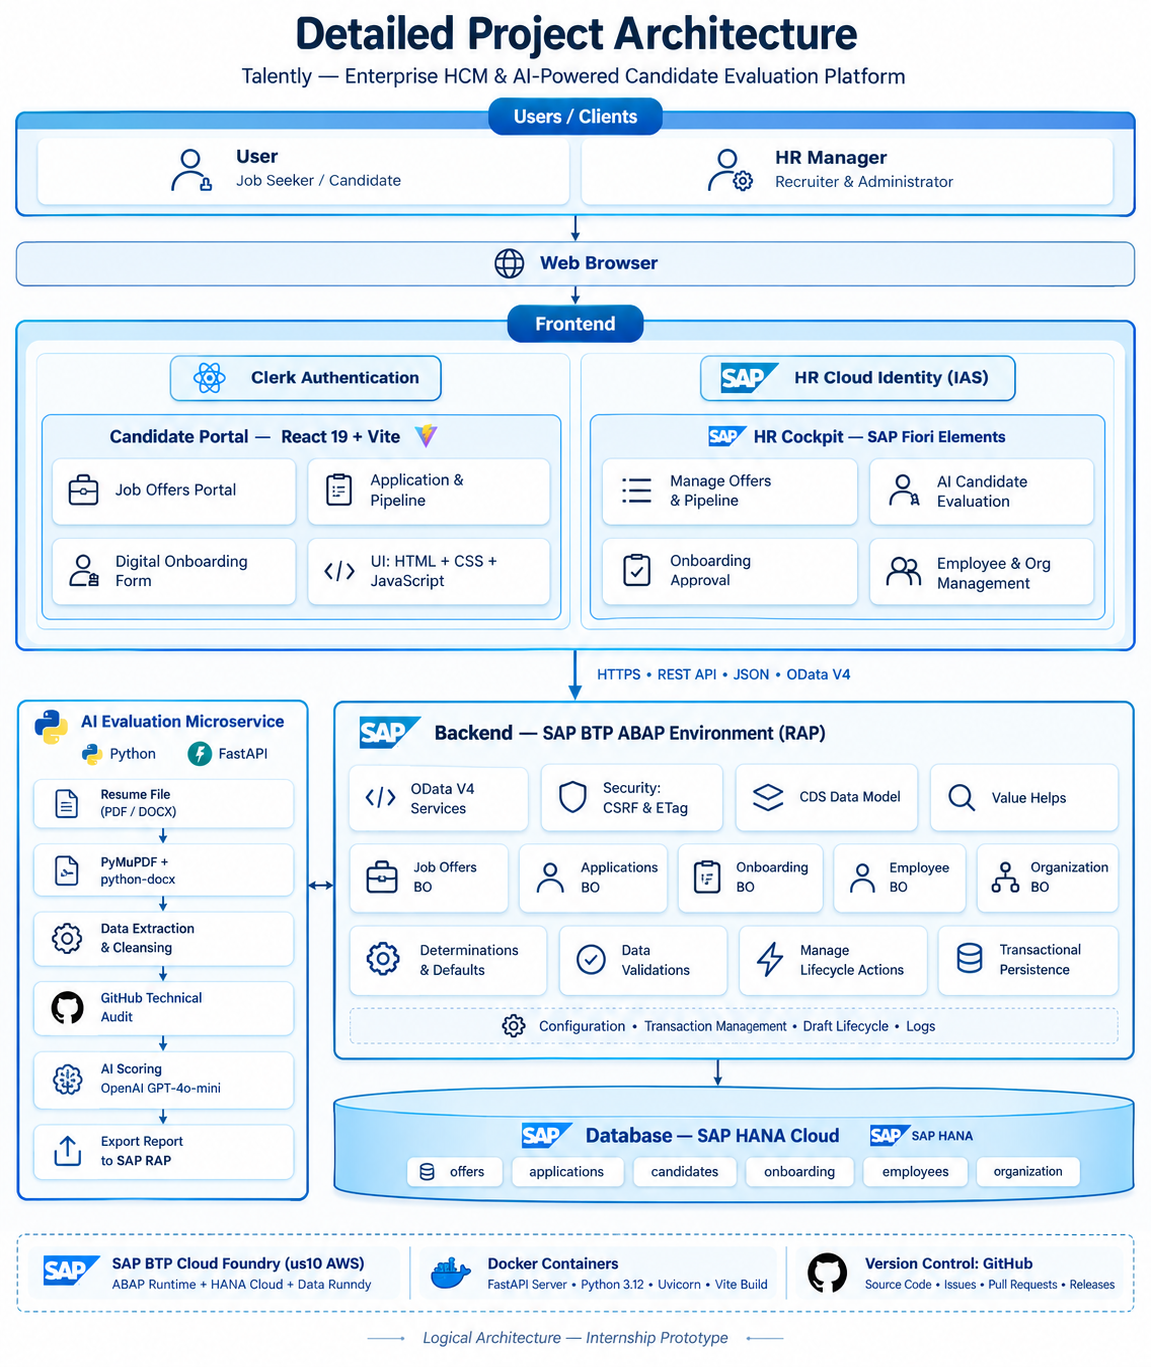
\includegraphics[width=0.78\textwidth]{Figures/global_architecture.png}
    \caption{Global System Architecture of the Talently Platform}
    \label{fig:global_architecture}
\end{figure}

\begin{itemize}
    \item \textbf{Users:} two profiles access the platform through a web browser: the \emph{candidate} (job seeker) and the \emph{HR manager} (recruiter and administrator).
    \item \textbf{Frontend:} two separate portals, each with its own identity provider. The \textbf{candidate portal} (React 19 + Vite) offers the job board, the application and pipeline tracking, and the onboarding form, with authentication handled by \textbf{Clerk}. The \textbf{HR cockpit} (SAP Fiori Elements) offers offer and pipeline management, AI candidate evaluation, onboarding approval, and employee and organization management, with authentication handled by \textbf{SAP Cloud Identity Services (IAS)}.
    \item \textbf{Backend (SAP BTP ABAP Environment, RAP):} the system of record. It exposes OData V4 services protected by CSRF tokens and ETags, and implements the five business domains (job offers, applications, onboarding, employees, and organization) as RAP business objects with determinations, validations, and lifecycle actions.
    \item \textbf{AI evaluation microservice (Python, FastAPI):} analyzes resumes, audits the candidate's GitHub activity, scores the candidate with GPT-4o-mini, and returns the result to the portal, which writes it to the backend.
    \item \textbf{Database (SAP HANA Cloud):} stores the active and draft records of all HR domains.
    \item \textbf{Infrastructure:} SAP BTP Cloud Foundry (us10 region) hosts the ABAP runtime and HANA Cloud, the FastAPI service is packaged as a Docker image, and GitHub manages the source code. In the prototype, the AI microservice and the candidate portal run on the development machine, the portal through the Vite development server and its proxy.
\end{itemize}

All exchanges use HTTPS and JSON: REST for the AI microservice and OData V4 for the SAP backend.

The end-to-end flow is as follows. A candidate applies through the portal, and the application is stored in SAP. The resume is sent to the AI microservice, whose score is written back to the application. The recruiter reviews the candidate in the Fiori cockpit, moves them through the pipeline, and accepts them. The candidate then completes the onboarding form, and its approval by HR creates the employee master record in a single RAP transaction, without any manual re-entry.

% ──────────────────────────────────────────────
\subsection{Simplified Backend Architecture}
\label{subsec:backend_architecture}
% ──────────────────────────────────────────────

The backend is built with the ABAP RESTful Application Programming Model (RAP)~\cite{sap_rap} on the SAP BTP ABAP Environment~\cite{sap_btp_abap}, using the \emph{managed scenario with draft}. In this scenario, the developer declares the data model and the business rules, while the SAP framework handles request processing, transactional buffering, locking, draft storage, and database access. Figure~\ref{fig:backend_architecture} shows the four layers of the backend.

\begin{figure}[htbp]
    \centering
    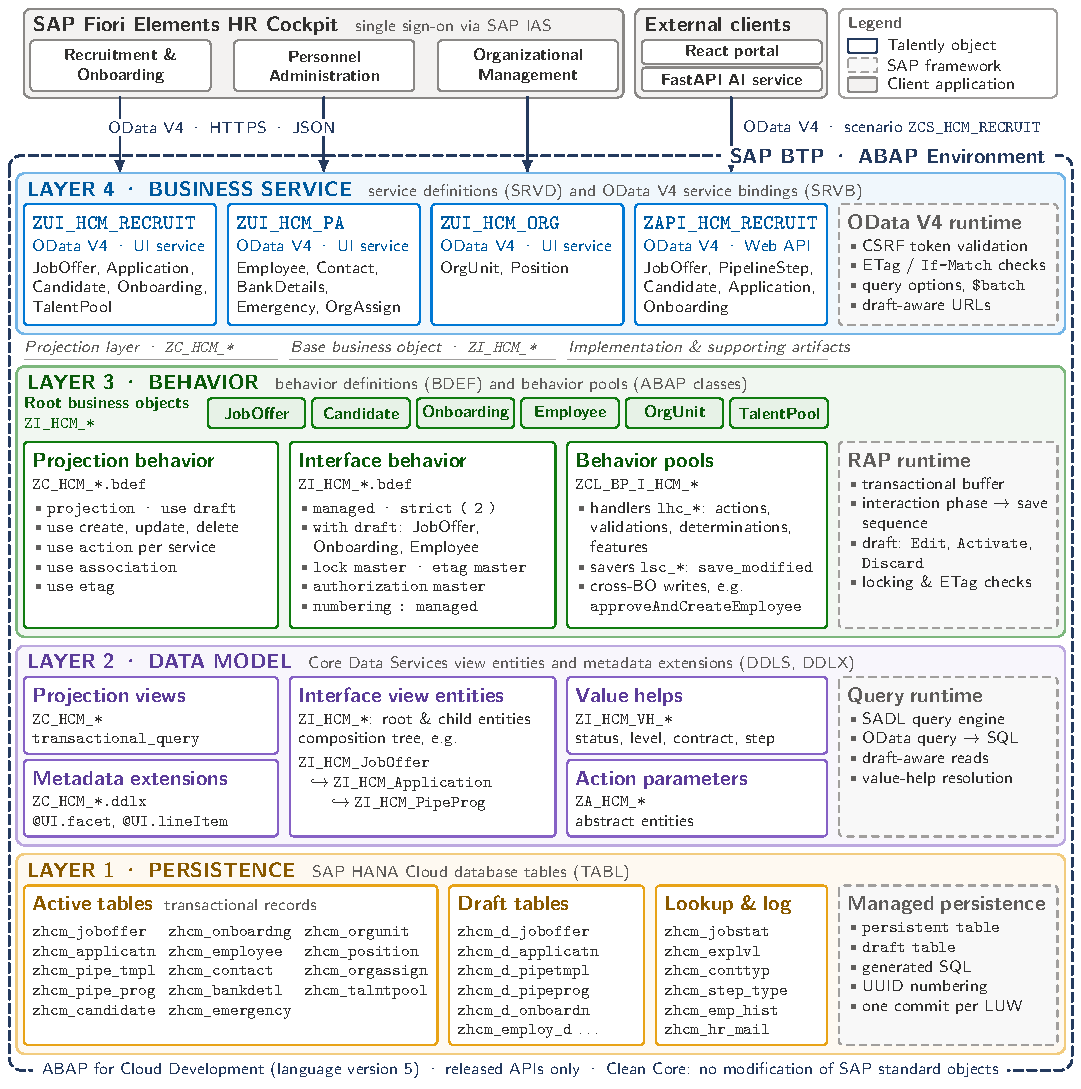
\includegraphics[width=\textwidth]{Figures/backend_architecture.pdf}
    \caption{ABAP RAP Backend -- Four-Layer Architecture}
    \label{fig:backend_architecture}
\end{figure}

\begin{itemize}
    \item \textbf{Business service layer:} service definitions (SRVD) and OData V4~\cite{odata} service bindings (SRVB). Three UI services serve the Fiori cockpit (\code{ZUI_HCM_RECRUIT}, \code{ZUI_HCM_PA}, \code{ZUI_HCM_ORG}), and one Web API, \code{ZAPI_HCM_RECRUIT}, is published through the communication scenario \code{ZCS_HCM_RECRUIT} for external integrations. In the prototype, the candidate portal calls the recruitment service \code{ZUI_HCM_RECRUIT} through a development proxy, both for the applications and for writing back the AI results.
    \item \textbf{Behavior layer:} behavior definitions (BDEF) declare, for each business object, its operations, actions, validations, determinations, locking, ETag, and draft handling (\code{managed}, \code{strict ( 2 )}, \code{with draft}). The logic is implemented in behavior pools (\code{ZCL_BP_I_HCM_*}), split into handler classes (\code{lhc_*}) and saver classes (\code{lsc_*}).
    \item \textbf{Data model layer:} Core Data Services (CDS) view entities~\cite{sap_cds}. Interface views (\code{ZI_HCM_*}) define the canonical data model and its compositions, projection views (\code{ZC_HCM_*}) adapt it to each service, and metadata extensions carry the Fiori UI annotations.
    \item \textbf{Persistence layer:} SAP HANA Cloud tables: active tables (\code{zhcm_joboffer}, \code{zhcm_applicatn}, \code{zhcm_employee}, \ldots), draft tables (\code{zhcm_d_joboffer}, \ldots), and lookup and log tables (\code{zhcm_jobstat}, \code{zhcm_emp_hist}, \ldots).
\end{itemize}

The dashed boxes of Figure~\ref{fig:backend_architecture} show what the SAP framework provides at each layer (CSRF and ETag checks, transactional buffer, query engine, SQL generation), so the Talently code contains only business rules. The backend is written in ABAP for Cloud Development using released APIs only, so no SAP standard object is modified.

\paragraph*{Business objects.} Table~\ref{tab:bo_catalogue} lists the six business objects of the backend. A child entity is created, locked, and saved together with its root: for example, an application belongs to its job offer, so locking an offer protects its whole recruitment pipeline. The candidate, the onboarding form, and the employee are separate roots because each has its own lifecycle. Draft handling is enabled only for the objects that HR users edit in several steps, and all keys are UUIDs generated by the framework.

\begingroup
\linespread{1}\selectfont
\renewcommand{\arraystretch}{1.4}
\begin{longtable}{@{}F{3.6cm}F{7.9cm}C{1.1cm}F{4.6cm}@{}}
\caption{Business Objects of the Talently Backend}\label{tab:bo_catalogue}\\
\toprule
\textbf{Business object} & \textbf{Child entities} & \textbf{Draft} & \textbf{Service} \\
\midrule
\endfirsthead
\toprule
\textbf{Business object} & \textbf{Child entities} & \textbf{Draft} & \textbf{Service} \\
\midrule
\endhead
\bottomrule
\endlastfoot
\code{ZI_HCM_OrgUnit} & \code{ZI_HCM_Position} & Yes & \code{ZUI_HCM_ORG} \\
\code{ZI_HCM_JobOffer} & \code{ZI_HCM_PipeTmpl}, \code{ZI_HCM_Application} $\rightarrow$ \code{ZI_HCM_PipeProg} & Yes & \code{ZUI_HCM_RECRUIT}, \code{ZAPI_HCM_RECRUIT} \\
\code{ZI_HCM_Candidate} & -- & No & \code{ZUI_HCM_RECRUIT}, \code{ZAPI_HCM_RECRUIT} \\
\code{ZI_HCM_Onboarding} & -- & Yes & \code{ZUI_HCM_RECRUIT}, \code{ZAPI_HCM_RECRUIT} \\
\code{ZI_HCM_Employee} & \code{ZI_HCM_Contact}, \code{ZI_HCM_BankDetl}, \code{ZI_HCM_Emergency}, \code{ZI_HCM_OrgAssign} & Yes & \code{ZUI_HCM_PA} \\
\code{ZI_HCM_TalentPool} & -- & No & \code{ZUI_HCM_RECRUIT} \\
\end{longtable}
\endgroup

\paragraph*{Main business actions.} Table~\ref{tab:main_actions} summarizes the main actions. Their availability is computed for each instance (feature control): for example, \emph{Publish} is only enabled for a draft or closed offer, and \emph{Accept to Post} only when the candidate has reached the last pipeline step. In addition, validations block inconsistent data before it is saved: mandatory fields, application deadline, vacant position, duplicate applications, and at least one pipeline step before publishing.

\begingroup
\linespread{1}\selectfont
\renewcommand{\arraystretch}{1.4}
\begin{longtable}{@{}F{5.6cm}F{2.8cm}F{9.1cm}@{}}
\caption{Main Business Actions of the Backend}\label{tab:main_actions}\\
\toprule
\textbf{Action} & \textbf{Business object} & \textbf{Effect} \\
\midrule
\endfirsthead
\toprule
\textbf{Action} & \textbf{Business object} & \textbf{Effect} \\
\midrule
\endhead
\bottomrule
\endlastfoot
\code{publishOffer}, \code{closeOffer} & Job offer & Publishes the offer on the portal or closes it. \\
\code{applyToJob} & Candidate & Creates an application at the first pipeline step. \\
\code{setAIEvaluation}, \code{evaluateWithAI} & Application & Stores the AI score, recommendation, and summary, or flags the application for a new evaluation (\emph{PENDING}). \\
\code{passToNextStep} & Application & Moves the candidate to the next pipeline step. \\
\code{acceptToPost} & Application & Accepts the candidate, prepares the onboarding form, and closes the offer when all positions are filled. \\
\code{rejectCandidate} & Application & Rejects the candidate and adds them to the talent pool. \\
\code{approveAndCreateEmployee} & Onboarding & Creates the employee master record with contact, bank, emergency, and assignment data. \\
\code{promoteEmployee}, \code{transferEmployee}, \code{terminateEmployee} & Employee & Records personnel events in the employment history. \\
\end{longtable}
\endgroup

\paragraph*{Transaction model.} RAP executes every request in two phases. During the \emph{interaction phase}, the handler classes apply the changes to an in-memory transactional buffer. During the \emph{save sequence}, all validations run; if they pass, the buffer is written and committed as a single database transaction, otherwise nothing is saved. Because RAP forbids database writes during the interaction phase, the records of other business objects are written by the saver classes during the save sequence, following a \emph{buffer-then-save} pattern. For example, \code{approveAndCreateEmployee} buffers the form data, and the saver class \code{lsc_ZI_HCM_ONBOARDING} creates the employee during the save sequence. The hiring is therefore atomic: either the employee record is fully created and the form approved, or nothing changes.

\keepwith{0.9\textheight}
\subsubsection{Sequence Diagram: Job Offer Management}
\label{subsubsec:seq_job_offer}

\begin{figure}[H]
    \centering
    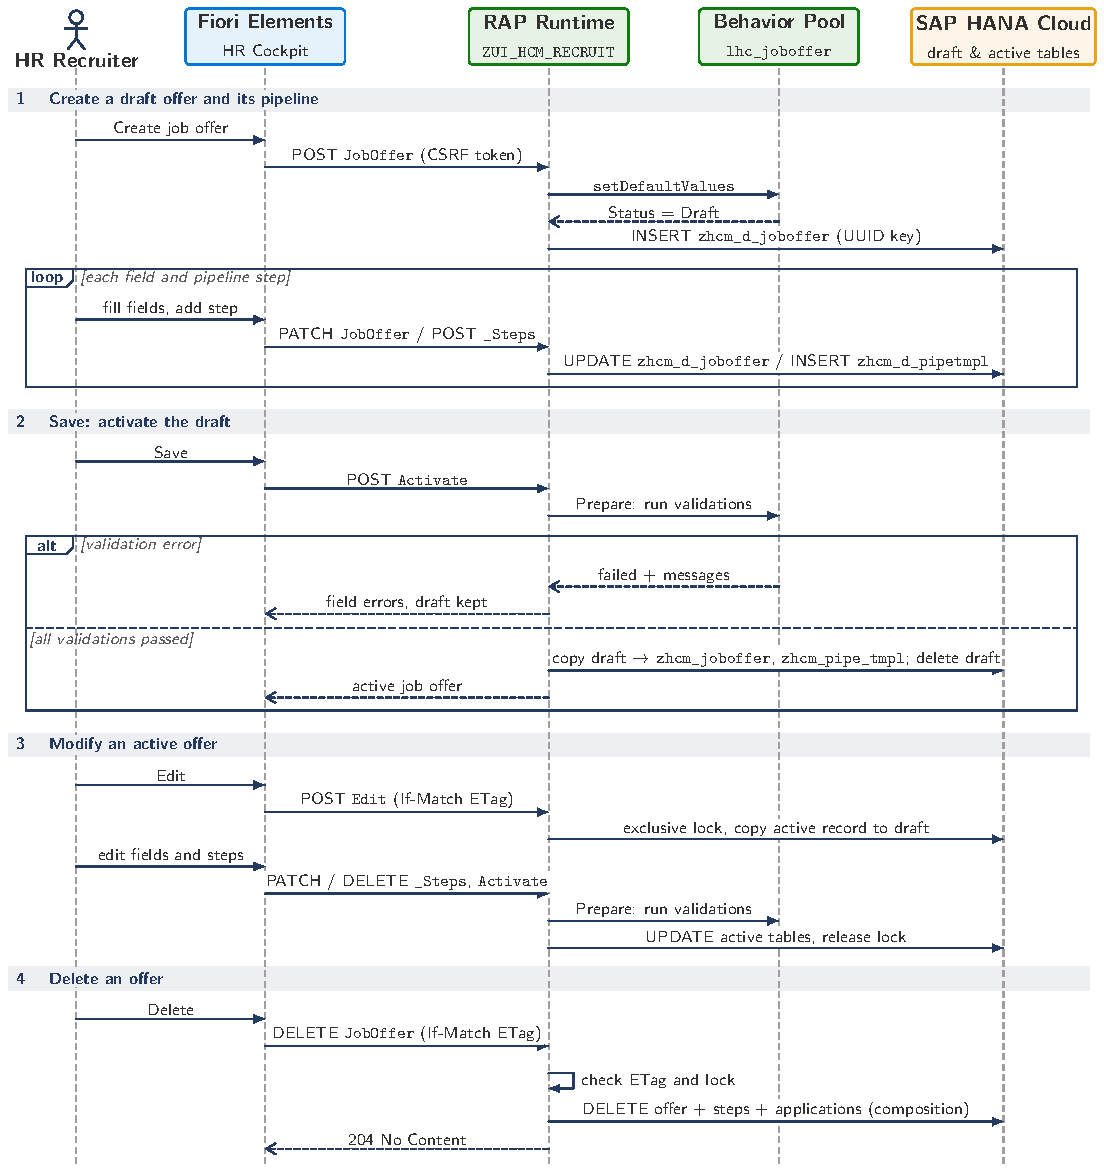
\includegraphics[width=\textwidth]{Figures/seq_job_offer.pdf}
    \caption{Sequence Diagram -- Job Offer Management (Create, Modify, Delete)}
    \label{fig:seq_job_offer}
\end{figure}

The diagram follows the four operations of a recruiter on a job offer:

\begin{enumerate}
    \item \textbf{Create:} the RAP runtime creates a draft with a UUID key and the status \emph{Draft}; the fields and pipeline steps are saved automatically in the draft tables.
    \item \textbf{Save:} the \emph{Activate} action runs the validations. On error, the draft is kept; otherwise, the offer and its steps are copied to the active tables in one transaction.
    \item \textbf{Modify:} the \emph{Edit} action locks the offer and copies it into a new draft, so two recruiters cannot change it at the same time.
    \item \textbf{Delete:} protected by the ETag, it removes the offer together with its pipeline steps and applications (composition).
\end{enumerate}

% ──────────────────────────────────────────────
\subsection{Simplified AI Agent Architecture}
\label{subsec:ai_architecture}
% ──────────────────────────────────────────────

The AI evaluation engine is a stateless Python microservice built with FastAPI. It is kept outside SAP so that slow or unpredictable LLM processing never affects ERP transactions. It receives a resume together with the target job offer, and returns a structured, explainable score. Figure~\ref{fig:ai_engine} shows its processing pipeline.

\begin{figure}[htbp]
    \centering
    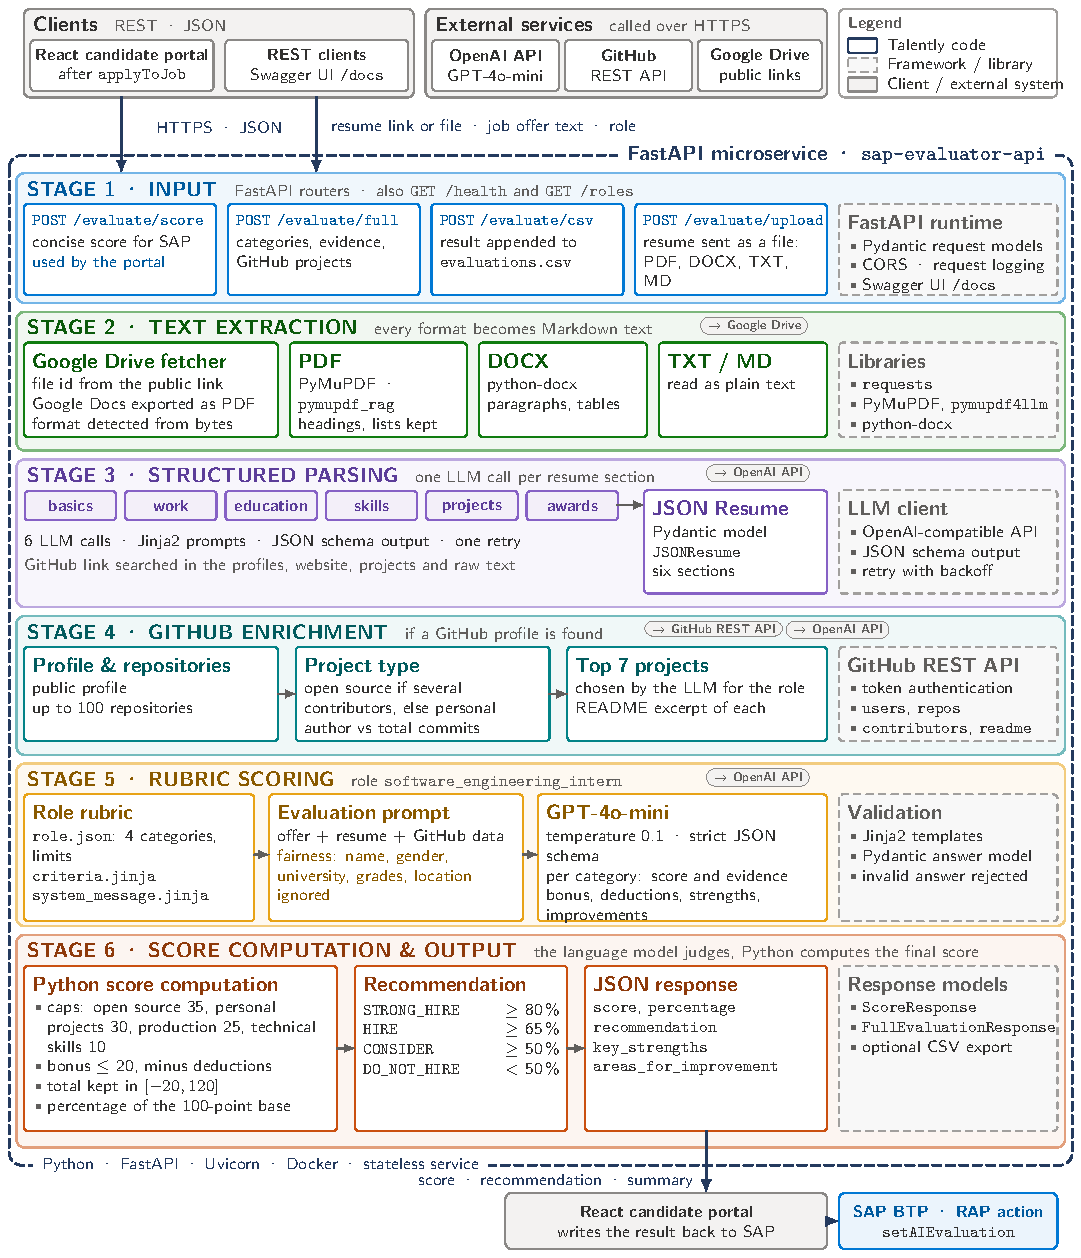
\includegraphics[width=0.97\textwidth]{Figures/ai_evaluation_engine.pdf}
    \caption{AI Evaluation Microservice -- Resume Scoring Pipeline}
    \label{fig:ai_engine}
\end{figure}

The pipeline runs in six stages:

\begin{enumerate}
    \item \textbf{Input:} the resume is received as a Google Drive link or an uploaded file (PDF, DOCX, TXT, or MD), together with the job offer description, through the REST endpoints \code{/evaluate/score} and \code{/evaluate/full}.
    \item \textbf{Text extraction:} the document is downloaded from Google Drive (or received as a file) and converted into clean Markdown (PyMuPDF for PDF, python-docx for Word).
    \item \textbf{Structured parsing:} six LLM calls extract the basics, work experience, education, skills, projects, and awards into the standard JSON Resume model~\cite{jsonresume}, validated with Pydantic.
    \item \textbf{GitHub enrichment:} the candidate's GitHub profile is detected automatically. The GitHub API~\cite{github_api} provides the repositories and commit statistics, each project is classified as open source or personal, the LLM selects the seven most relevant ones, and their README quality is checked.
    \item \textbf{Rubric scoring:} GPT-4o-mini (temperature 0.1) evaluates the candidate against the rubric of the target role, defined in Jinja2 templates, and against the text of the job offer. The text sent to the model contains no personal identifiers: the name, contact details, location, institution, and grades are left out. The model must answer in a strict JSON schema~\cite{openai_structured} with evidence for each category, key strengths, and areas for improvement.
    \item \textbf{Score computation and write-back:} the final score is computed in Python (category caps, bonus, deductions, and a total bounded to $[-20, 120]$), a recommendation is derived, and the result is returned to the portal, which writes it to the application in SAP through the RAP action \code{setAIEvaluation}.
\end{enumerate}

\begingroup
\linespread{1}\selectfont
\renewcommand{\arraystretch}{1.4}
\begin{longtable}{@{}F{13.5cm}C{4.0cm}@{}}
\caption{Evaluation Rubric of the Software Engineering Intern Role}\label{tab:ai_rubric}\\
\toprule
\textbf{Criterion} & \textbf{Points} \\
\midrule
\endfirsthead
\toprule
\textbf{Criterion} & \textbf{Points} \\
\midrule
\endhead
\midrule
\multicolumn{2}{@{}F{17.5cm}@{}}{Recommendation: \textbf{STRONG\_HIRE} ($\geq$ 80\,\%), \textbf{HIRE} ($\geq$ 65\,\%), \textbf{CONSIDER} ($\geq$ 50\,\%), \textbf{DO\_NOT\_HIRE} ($<$ 50\,\%).} \\
\bottomrule
\endlastfoot
Open source contributions & 0 -- 35 \\
Personal projects & 0 -- 30 \\
Production experience & 0 -- 25 \\
Technical skills & 0 -- 10 \\
Bonus (e.g., Google Summer of Code, startup experience, portfolio) & up to +20 \\
Deductions (e.g., tutorial-only projects, projects without links or README) & $-N$ \\
\end{longtable}
\endgroup

Two design choices make the evaluation trustworthy. First, the LLM judges but Python calculates: the final number is computed deterministically from the LLM's structured answer, so it always respects the rubric limits. Second, the evaluation is designed to be fair: the prompt forbids using the candidate's name, gender, university, grades, or location, and these details are not even sent to the scoring model. This second measure was added after the fairness test presented in Chapter~\ref{chap:implementation}. The score only supports the recruiter, who keeps the final decision in the Fiori cockpit.

\keepwith{0.8\textheight}
\subsubsection{Sequence Diagram: Candidate Application and AI Evaluation}
\label{subsubsec:seq_ai_evaluation}

\begin{figure}[H]
    \centering
    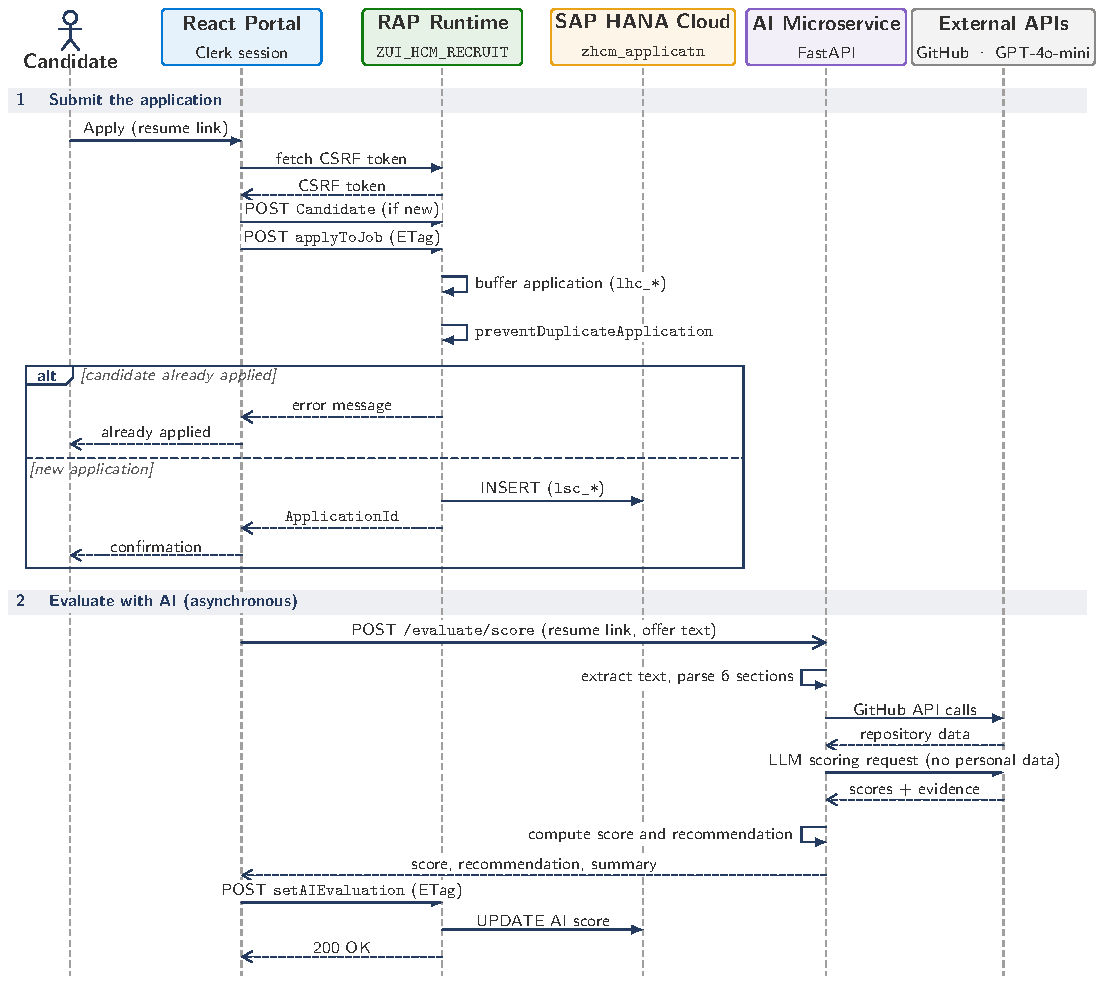
\includegraphics[width=\textwidth]{Figures/seq_ai_evaluation.pdf}
    \caption{Sequence Diagram -- Candidate Application and AI Evaluation}
    \label{fig:seq_ai_evaluation}
\end{figure}

The scenario runs in two phases:

\begin{enumerate}
    \item \textbf{Application:} the portal obtains a CSRF token and calls \code{applyToJob} on the service \code{ZUI_HCM_RECRUIT}. The application is inserted only if the duplicate-application check passes.
    \item \textbf{AI evaluation:} the portal sends the resume link and the offer text to the AI microservice asynchronously, so the candidate does not wait. The service parses the resume, queries GitHub and GPT-4o-mini, and computes the score; the portal then writes the result back through \code{setAIEvaluation}, where it becomes visible to the recruiter in the Fiori cockpit.
\end{enumerate}

% ──────────────────────────────────────────────
\subsection{UI/UX Expectations}
\label{subsec:uiux}
% ──────────────────────────────────────────────

Talently has two interfaces for two audiences. The candidate portal is a free React design focused on simplicity and self-service, while the HR cockpit follows the SAP Fiori design guidelines~\cite{sap_fiori_design}: its screens are generated by SAP Fiori Elements~\cite{sap_fiori_elements} from the annotations of the CDS projection views, using the standard \emph{List Report} and \emph{Object Page} floorplans. Figure~\ref{fig:routing_tree} shows the navigation of both interfaces.

\begin{figure}[H]
\centering
\begin{minipage}{0.97\textwidth}
\linespread{1}\selectfont\footnotesize
\begin{verbatim}
Candidate Portal (React 19, React Router)
/                     Job Board: published offers, search and filters
|-- /jobs/:id         Job Details: description, skills, pipeline steps, apply form
|-- /applications     My Applications: offers applied to, progress tracking
|-- /onboarding/:id   Onboarding Form: personal, legal, bank and emergency data
|-- /talent-pool      Talent Pool: non-selected candidates (HR role only)
`-- *                 Fallback page
Sign-in / Sign-up     Clerk modal, available from every page

HR Cockpit (SAP Fiori Elements: List Report -> Object Page)
Recruitment & Onboarding  (ZUI_HCM_RECRUIT)
|-- Job Offers -> Job Offer: General Information, Pipeline Steps, Applications
|   `-- Application: details, AI score, Pipeline Progress
|-- Onboarding Forms -> Onboarding Form: personal, bank and legal data
`-- Talent Pool
Personnel Administration  (ZUI_HCM_PA)
`-- Employees -> Employee: Contact, Bank Details, Emergency, Assignment
Organizational Management (ZUI_HCM_ORG)
`-- Organizational Units -> Organizational Unit: Positions
\end{verbatim}
\end{minipage}
\caption{Application Routing Tree of the Candidate Portal and the HR Cockpit}
\label{fig:routing_tree}
\end{figure}

The main screens were first sketched as low-fidelity wireframes with Excalidraw, which fixed the layout of each screen and the information it shows. The sketches were then refined into higher-fidelity mockups. Figure~\ref{fig:wireframes_portal} shows the mockup of the job board of the candidate portal, with its four zones: navigation header, search and filter bar, filter sidebar, and job card. Figure~\ref{fig:wireframes_cockpit} shows the mockup of the job offers list of the HR cockpit, built on the standard Fiori List Report floorplan: header, filter bar, table toolbar with the lifecycle actions, and data table.

\begin{figure}[H]
    \centering
    \imgslot{Figures/wireframes/portal_wireframes.png}{0.92\textwidth}{6cm}
    \caption{Mockup of the Job Board of the Candidate Portal}
    \label{fig:wireframes_portal}
\end{figure}

\begin{figure}[H]
    \centering
    \imgslot{Figures/wireframes/cockpit_wireframes.png}{0.92\textwidth}{6cm}
    \caption{Mockup of the Job Offers List of the HR Cockpit}
    \label{fig:wireframes_cockpit}
\end{figure}

\keepwith{0.92\textheight}
% ═══════════════════════════════════════════════
\section{Detailed Design}
\label{sec:detailed_design}
% ═══════════════════════════════════════════════

% ──────────────────────────────────────────────
\subsection{Class Diagram}
\label{subsec:class_diagram}
% ──────────────────────────────────────────────

\begin{figure}[H]
    \centering
    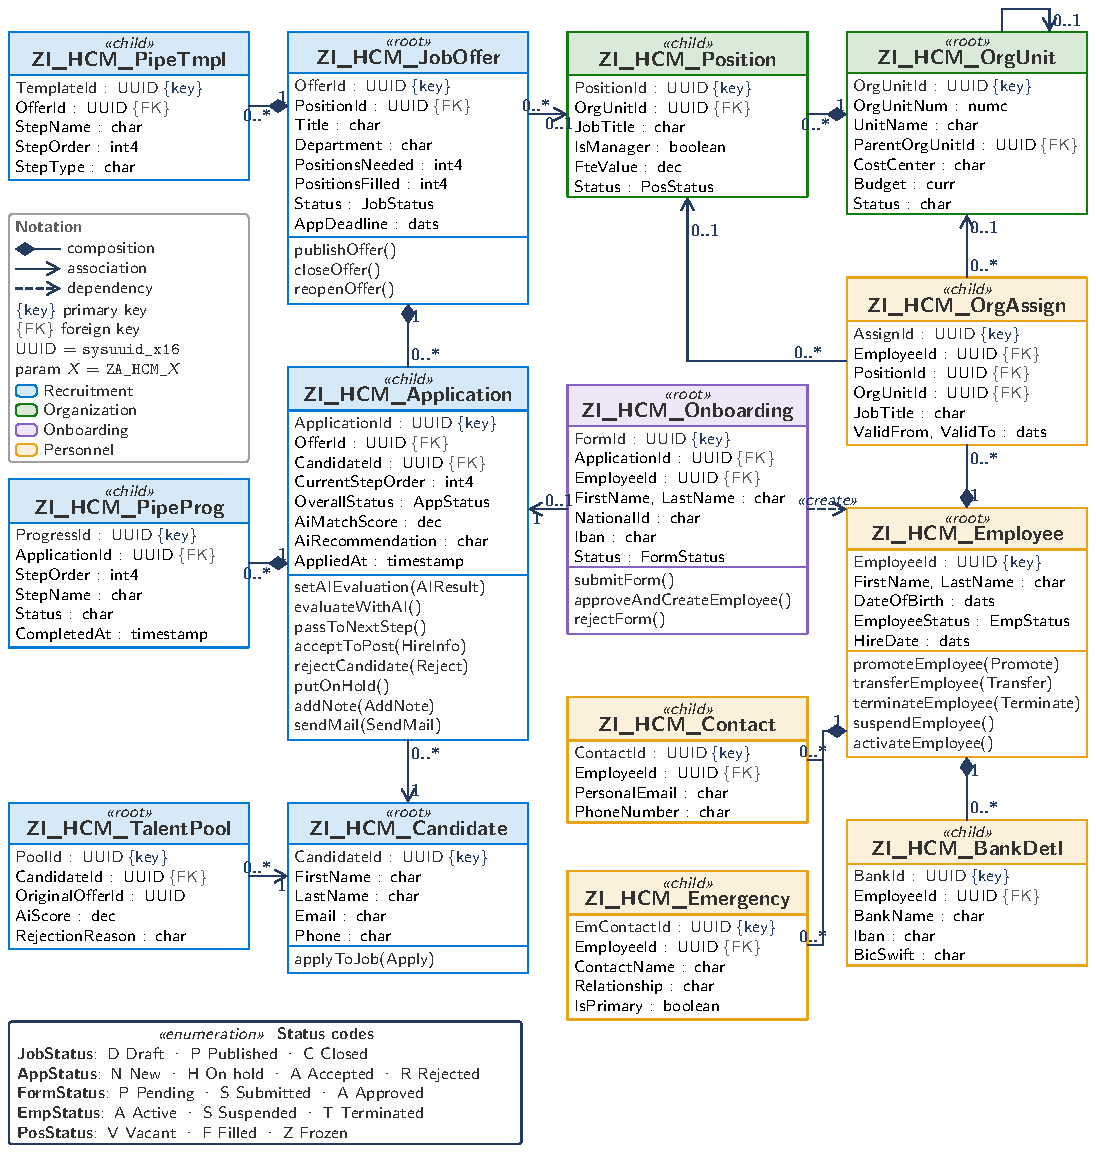
\includegraphics[width=\textwidth]{Figures/class_diagram.pdf}
    \caption{Class Diagram of the Talently Data Model (CDS Interface Views)}
    \label{fig:class_diagram}
\end{figure}

Each class is a CDS interface view (\code{ZI_HCM_*}) showing its main fields and its RAP actions, colored by domain. Three types of relationships are used:

\begin{itemize}
    \item \textbf{Composition} (filled diamond): the child is created, locked, and deleted with its parent (1 to 0..*): job offer to pipeline steps and applications, application to progress records, organizational unit to positions, and employee to contact, bank, emergency, and assignment records.
    \item \textbf{Association} (arrow): a link between independent objects: application to candidate (0..* to 1), onboarding form to application (0..1 to 1), job offer to position (0..* to 0..1), talent-pool entry to candidate, assignment to position and organizational unit, and organizational unit to its parent unit (0..1).
    \item \textbf{Dependency} (dashed arrow): the onboarding form creates the employee through \code{approveAndCreateEmployee}.
\end{itemize}

All keys are UUIDs, the \{FK\} fields implement the associations, and the status codes are listed in the enumeration box.

% ─────────────────────────────────────────────
\section*{Conclusion}
\addcontentsline{toc}{section}{Conclusion}
% ─────────────────────────────────────────────

This chapter presented the design of Talently. The global architecture separates the SAP BTP backend, which holds all business data and rules, from the AI microservice and the two user interfaces. The RAP backend was described through its layers, business objects, actions, and transaction model, and the AI engine through its six-stage pipeline and scoring rubric. The sequence diagrams, the routing tree, and the class diagram detailed the main scenarios and the data model. The next chapter presents the tools used to build the solution, demonstrates it end to end, and evaluates it.

\fussy


\chapter{Implementation, Testing, and Results}
\label{chap:implementation}

% ── chapter-local helpers ─────────────────────────────────────────────
\providecommand{\code}[1]{\texttt{\detokenize{#1}}}
\providecommand{\imgslot}[3]{\IfFileExists{#1}{\includegraphics[width=#2]{#1}}%
  {\fbox{\parbox[c][#3][c]{\dimexpr#2-2\fboxsep-2\fboxrule\relax}{\centering\color{gray}\footnotesize\texttt{\detokenize{#1}}}}}}
% all measured values are filled in (placeholders are no longer highlighted)
\newcommand{\tofill}[1]{#1}
% logo figure:  \logo{file}{caption}{label}
\newcommand{\logo}[3]{%
  \begin{figure}[H]\centering
    \IfFileExists{Figures/logos/#1}{\includegraphics[width=4.5cm]{Figures/logos/#1}}%
      {\imgslot{Figures/logos/#1}{7cm}{2.2cm}}
    \caption{#2}\label{#3}
  \end{figure}}
% screenshot figure:  \shot[max height, default 0.40]{file}{caption}{label}
% (92% of the text width, at most 40% of the page height, thin frame around the capture)
\newcommand{\shot}[4][0.40]{%
  \begin{figure}[H]\centering
    \IfFileExists{Figures/screens/#2}%
      {{\setlength{\fboxsep}{0pt}\setlength{\fboxrule}{0.4pt}%
        \fbox{\includegraphics[width=\dimexpr0.92\textwidth-0.8pt\relax,height=#1\textheight,keepaspectratio]{Figures/screens/#2}}}}%
      {\imgslot{Figures/screens/#2}{\textwidth}{7cm}}
    \caption{#3}\label{#4}
  \end{figure}}
% technology heading (bold bullet on its own line, as in the reference report)
\newcommand{\tech}[1]{\par\medskip\noindent{\large\bfseries$\bullet$\ #1}\par\nopagebreak}
\newcolumntype{F}[1]{>{\footnotesize\raggedright\arraybackslash}p{#1}}
\setlength{\LTcapwidth}{\textwidth}
\sloppy

% ─────────────────────────────────────────────
\section*{Introduction}
\addcontentsline{toc}{section}{Introduction}
% ─────────────────────────────────────────────

This chapter presents the realization of Talently. It first introduces the tools and technologies used to build the platform. It then demonstrates the solution through a complete end-to-end scenario, from the creation of the organizational structure to the creation of a new employee. Finally, it presents the tests carried out and validates the functional and non-functional requirements defined in Chapter~\ref{chap:analysis_specifications}.

\newpage

% ═══════════════════════════════════════════════
\section{Development Environment}
\label{sec:dev_environment}
% ═══════════════════════════════════════════════

The platform combines the SAP cloud ecosystem, used for the transactional core and the HR cockpit, with open-source web and AI technologies, used for the candidate portal and the evaluation engine.

% ──────────────────────────────────────────────
\subsection{SAP Cloud Ecosystem}
\label{subsec:sap_ecosystem}
% ──────────────────────────────────────────────

\tech{SAP BTP ABAP Environment}
% LOGO: official "SAP Business Technology Platform" logo -> Figures/logos/sap_btp.png
\logo{sap_btp.png}{SAP Business Technology Platform Logo}{fig:logo_btp}
SAP Business Technology Platform (BTP) is SAP's cloud platform for building extensions around SAP solutions. Its ABAP Environment provides a managed ABAP runtime in the cloud, restricted to the ABAP Cloud development model and to released APIs. In Talently, it hosts the whole backend: the CDS data model, the behavior definitions, the business logic, and the OData V4 services. It was chosen because it allows the HCM extension to be built side by side with the ERP core, in line with SAP's Clean Core strategy.

\tech{SAP HANA Cloud}
% LOGO: official "SAP HANA Cloud" logo -> Figures/logos/sap_hana_cloud.png
\logo{sap_hana_cloud.png}{SAP HANA Cloud Logo}{fig:logo_hana}
SAP HANA Cloud is the in-memory, column-oriented database provided with the ABAP Environment. It stores the active and draft tables of all Talently business objects. Its in-memory processing gives fast reads for the Fiori list reports, and it is fully managed by the platform, so no database administration was required.

\tech{Eclipse with ABAP Development Tools (ADT)}
% LOGO: Eclipse IDE logo (optionally with the "ABAP Development Tools" text) -> Figures/logos/eclipse_adt.png
\logo{eclipse_adt.png}{Eclipse and ABAP Development Tools Logo}{fig:logo_adt}
ABAP Development Tools (ADT) is the official Eclipse-based environment for ABAP Cloud development. It was used to create and activate all development objects (tables, CDS views, behavior definitions, classes, service definitions, and service bindings), to preview the Fiori applications, and to debug the business logic. The sources were versioned with abapGit~\cite{abapgit}, which serializes the ABAP objects into files stored in the GitHub repository.

\tech{SAP Fiori Elements}
% LOGO: SAP Fiori logo -> Figures/logos/sap_fiori.png
\logo{sap_fiori.png}{SAP Fiori Logo}{fig:logo_fiori}
SAP Fiori Elements generates enterprise user interfaces from OData services and CDS annotations, using predefined floorplans such as the List Report and the Object Page. It was used to build the whole HR cockpit without writing user interface code: the layouts, tables, action buttons, and draft handling are derived from the metadata extensions of the projection views. This guarantees a consistent SAP user experience and greatly reduces development time.

\tech{SAP Cloud Identity Services}
SAP Cloud Identity Services (Identity Authentication Service, IAS) manages the identities of the HR users. It provides single sign-on to the Fiori cockpit and is the trusted identity provider of the ABAP Environment, so internal users never share the authentication mechanism of the external candidates.

% ──────────────────────────────────────────────
\subsection{Web, AI and DevOps Tooling}
\label{subsec:web_ai_tooling}
% ──────────────────────────────────────────────

\tech{React 19 and Vite}
% LOGO: React logo and Vite logo side by side -> Figures/logos/react_vite.png
\logo{react_vite.png}{Vite Logo}{fig:logo_react}
React is the most widely used JavaScript library for building component-based user interfaces, and Vite is a fast build tool and development server~\cite{react}. Together, they were used to build the candidate portal: job board, job details, application form, progress tracking, and onboarding form. React was chosen for its large ecosystem and component reuse, and Vite for its near-instant reload during development and its optimized production build.

\tech{Tailwind CSS}
% LOGO: Tailwind CSS logo -> Figures/logos/tailwind.png
\logo{tailwind.png}{Tailwind CSS Logo}{fig:logo_tailwind}
Tailwind CSS is a utility-first CSS framework. It was used to style the portal directly inside the components and to make every page responsive, without maintaining separate style sheets.

\tech{Clerk}
% LOGO: Clerk logo -> Figures/logos/clerk.png
\logo{clerk.png}{Clerk Logo}{fig:logo_clerk}
Clerk is an authentication service for web applications~\cite{clerk}. It provides the sign-in and sign-up screens, social login, and session management of the candidate portal. Delegating candidate authentication to Clerk keeps external identities separate from the SAP identity provider and avoids implementing password management.

\tech{Python 3.12 and FastAPI}
% LOGO: Python logo and FastAPI logo side by side -> Figures/logos/python_fastapi.png
\logo{python_fastapi.png}{FastAPI Logo}{fig:logo_fastapi}
FastAPI is a modern Python framework for building REST APIs~\cite{fastapi}. It validates every request and response with Pydantic models and automatically generates interactive documentation (Swagger). It was chosen for the AI microservice because Python offers the richest ecosystem for document processing and LLM integration, and because FastAPI is fast, lightweight, and easy to test.

\tech{OpenAI GPT-4o-mini}
% LOGO: OpenAI logo -> Figures/logos/openai.png
\logo{openai.png}{OpenAI Logo}{fig:logo_openai}
GPT-4o-mini is a compact large language model from OpenAI. It parses the resume sections, selects the most relevant GitHub projects, and scores the candidate against the rubric. It was chosen for its good reasoning quality at a low cost per evaluation and for its support of structured outputs, which forces the model to answer in a strict JSON schema~\cite{openai_structured}.

\tech{PyMuPDF and python-docx}
% LOGO: PyMuPDF logo (python-docx has none; the PyMuPDF logo alone is fine) -> Figures/logos/pymupdf.png
\logo{pymupdf.png}{PyMuPDF Logo}{fig:logo_pymupdf}
PyMuPDF~\cite{pymupdf} and python-docx are Python libraries for reading PDF and Word documents. They convert the submitted resumes into clean Markdown text, preserving headings and lists, before the text is sent to the language model.

\tech{Docker}
% LOGO: Docker logo -> Figures/logos/docker.png
\logo{docker.png}{Docker Logo}{fig:logo_docker}
Docker packages an application with all its dependencies into a portable container. The AI microservice is delivered as a Docker image, so it runs identically on the development machine and on any server, independently of the local Python installation.

\tech{Git and GitHub}
% LOGO: Git logo and GitHub logo side by side -> Figures/logos/git_github.png
\logo{git_github.png}{GitHub Logo}{fig:logo_github}
Git was used for version control and GitHub as the central repository of the three components of the project: the ABAP sources (through abapGit), the AI microservice, and the React portal. GitHub also kept the full history of every change.

% ═══════════════════════════════════════════════
\section{End-to-End Walkthrough}
\label{sec:walkthrough}
% ═══════════════════════════════════════════════

This section demonstrates Talently through a complete scenario executed on the SAP BTP ABAP trial system. Two actors take part: the HR administrator, who works in the SAP Fiori applications of the HR cockpit, and the candidates, who use the React portal. The test data are three organizational units (Information Technology, SAP Development, and Data \& AI), three vacant positions in SAP Development, one job offer \emph{SAP ABAP Developer (RAP)} for two positions with a three-step pipeline, and two candidates with different profiles: Salma Idrissi, a junior developer with a first RAP experience, and Omar Tazi, a sales assistant without IT experience. The journey is the following:

\begin{enumerate}\setlength{\itemsep}{0pt}\setlength{\parsep}{0pt}
    \item \textbf{Organization:} the HR administrator models the organizational units and their vacant positions.
    \item \textbf{Job offer:} the HR administrator creates the job offer, defines its pipeline, and publishes it.
    \item \textbf{Application:} the candidates find the offer on the portal, sign in, and apply.
    \item \textbf{AI evaluation:} the AI engine scores each resume, and the HR administrator reviews the applications.
    \item \textbf{Decision:} the HR administrator moves the candidates through the pipeline, accepts one, and rejects the other.
    \item \textbf{Onboarding:} the accepted candidate completes the onboarding form, and the HR administrator reviews it.
    \item \textbf{Employee administration:} the approval creates the employee, who is then managed in the Personnel Administration application.
\end{enumerate}

Each screenshot is followed by a description of the actions performed by the user and of the options available on the screen.

% ──────────────────────────────────────────────
\subsection{Organizational Structure Setup}
\label{subsec:wt_org}
% ──────────────────────────────────────────────

The organization is modeled by the HR administrator in the \emph{Organizational Management} application, exposed by the service binding \code{ZUI_HCM_ORG}.

\shot[0.33]{org_unit_create.png}{Creation of an Organizational Unit in Draft Mode}{fig:wt_org_create}

The HR administrator opens the Organizational Management application and clicks \emph{Create} to add the first unit, Information Technology (Figure~\ref{fig:wt_org_create}). The object page opens in draft mode and has three sections, reached from the tabs at the top: \emph{Basic Data}, \emph{Financials \& Status}, and \emph{Positions}. The unit number (000001) is assigned automatically. The user enters the unit name, which is mandatory, a description, the cost center (CC-100), the budget with its currency (5,000 MAD), and the status, and can select a parent unit with the value help. Every change is kept in the draft, as the \emph{Draft updated} indicator shows, so no data is lost. The user saves the unit with the \emph{Create} button at the bottom of the page or cancels it with \emph{Discard Draft}.

\shot{org_units_first.png}{Organizational Units List After the First Creation}{fig:wt_org_list1}

After saving, the HR administrator returns to the list report, which now shows the Information Technology unit with its number, cost center, budget, and status (Figure~\ref{fig:wt_org_list1}). The filter bar at the top searches the units by editing status, unit number, unit name, or cost center: the user fills the filters and clicks \emph{Go}, and \emph{Adapt Filters} adds more filter fields. Above the table, \emph{Create} adds a new unit and \emph{Delete} removes the selected units. The settings icon changes the visible columns, and the export icon exports the list to a spreadsheet. The arrow at the end of a row opens the unit.

\shot{org_units_list.png}{List of the Three Organizational Units}{fig:wt_org_units}

The HR administrator repeats the same steps to create the units SAP Development (cost center CC-1100, budget 30,000 MAD) and Data \& AI (cost center CC-1200, budget 25,000 MAD). The list report now contains the three units, all with the status \emph{Active} (Figure~\ref{fig:wt_org_units}). At this stage, the units are still independent: the \emph{Parent Unit} column is empty, and the hierarchy is built in the next step by editing the two sub-units.

\shot{org_parent_valuehelp.png}{Value Help of the Parent Unit}{fig:wt_org_parent}

To build the hierarchy, the HR administrator opens SAP Development, clicks \emph{Edit}, and opens the value help of the \emph{Parent Unit} field (Figure~\ref{fig:wt_org_parent}). A dialog lists the existing units with their name, number, and cost center. The user can search a unit with the search field and \emph{Go}, display more filters with \emph{Show Filters}, select the parent by clicking its row, or close the dialog with \emph{Cancel}. Information Technology is selected as the parent of SAP Development, and the same is done for Data \& AI.

\shot{org_validation_parent.png}{Validation Error on the Parent Unit}{fig:wt_org_validation}

The business rules are checked when the draft is saved. If the HR administrator selects SAP Development as its own parent and clicks \emph{Save}, the backend validation blocks the save (Figure~\ref{fig:wt_org_validation}). The wrong field is highlighted in red, a banner asks to resolve the data inconsistencies, and the message popover, opened from the red counter at the bottom left, lists the errors, here \emph{An organizational unit cannot be its own parent}. Clicking a message leads to the related field, so the user corrects the value and saves again.

\shot{org_unit_display.png}{Data \& AI Unit in Display Mode}{fig:wt_org_display}

Once saved, the unit is displayed in read-only mode (Figure~\ref{fig:wt_org_display}). The Data \& AI unit now shows Information Technology as its parent unit, together with its description, cost center, budget, and status. In display mode, the header offers two buttons: \emph{Edit} (shortcut Ctrl+E), which opens a new draft of the unit, and \emph{Delete}, which removes it. The \emph{Positions} section is still empty, because positions are added in edit mode.

\shot{org_positions_edit.png}{Positions Section of SAP Development in Edit Mode}{fig:wt_org_pos_edit}

The HR administrator then opens SAP Development and clicks \emph{Edit} to create its positions (Figure~\ref{fig:wt_org_pos_edit}). In edit mode, the \emph{Positions} table offers the \emph{Create} button, which adds a new position, and \emph{Delete}, which removes the selected positions. For each position, the table shows the job title, which is mandatory, the manager flag, the full-time equivalent (FTE), the position budget, and the status. The unit stays in draft until the user saves it.

\shot{position_details.png}{Details of a Position}{fig:wt_position_detail}

Each position also has its own details page, linked to its unit by the breadcrumb \emph{SAP Development} at the top (Figure~\ref{fig:wt_position_detail}). The HR administrator enters the job title \emph{SAP ABAP Developer}, the FTE value (1.00), and the position budget (12,000 MAD), selects the status \emph{Vacant} in the drop-down list, and can tick \emph{Is Manager} for a management position. The \emph{Apply} button returns to the unit with the new position, and \emph{Delete} removes the position.

\shot{org_positions_one.png}{First Position in the Positions Table}{fig:wt_org_pos_one}

After \emph{Apply}, the position appears as a row of the \emph{Positions} table of SAP Development, where its fields can still be edited directly (Figure~\ref{fig:wt_org_pos_one}). The unit is still a draft, as the \emph{Draft} label next to its name shows. The HR administrator can add more positions with \emph{Create} and confirms all the changes with \emph{Save} at the bottom of the page, or cancels them with \emph{Discard Draft}.

\shot{org_positions.png}{Positions of the SAP Development Unit}{fig:wt_org_positions}

The HR administrator adds a second \emph{SAP ABAP Developer} position and one \emph{SAP Senior Developer} position (budget 18,000 MAD), then clicks \emph{Save} (Figure~\ref{fig:wt_org_positions}). The unit returns to display mode with its three positions, all with the status \emph{Vacant}. The two SAP ABAP Developer positions are the ones to fill through the recruitment, and the senior position can later be used for a promotion. The \emph{Edit} and \emph{Delete} buttons are available again in the header.

\shot{org_delete_confirm.png}{Deletion Request of an Organizational Unit}{fig:wt_org_delete}

Back in the list report, the \emph{Parent Unit} column now shows Information Technology for the two sub-units. To test the integrity rules, the HR administrator selects SAP Development and clicks \emph{Delete} (Figure~\ref{fig:wt_org_delete}). Before anything is deleted, a dialog asks for a confirmation and shows the name and number of the unit. The user confirms with \emph{Delete} or stops with \emph{Cancel}.

\shot{org_delete_refused.png}{Deletion Refused for a Unit That Still Has Positions}{fig:wt_org_delete_refused}

After the confirmation, the backend refuses the deletion and returns the error \emph{Cannot delete an organizational unit that still has positions} (Figure~\ref{fig:wt_org_delete_refused}). The same rule protects a unit that still has sub-units. The user closes the message with \emph{Close}, and the unit stays unchanged. In this way, a position can never lose its organizational unit.

% ──────────────────────────────────────────────
\subsection{Job Offer Creation and Publication}
\label{subsec:wt_offer}
% ──────────────────────────────────────────────

Recruitment starts in the \emph{Job Offers} application of the HR cockpit, exposed by the service binding \code{ZUI_HCM_RECRUIT}.

\shot{offer_list.png}{Job Offers List Report}{fig:wt_offer_list}

The HR administrator opens the Job Offers application, which is empty at the start of the scenario (Figure~\ref{fig:wt_offer_list}). The filter bar searches the offers by editing status, status, department, and title. For each offer, the table shows the title, the position, the department, the status, the number of positions needed and filled, and the validity date. The toolbar groups the actions of the offer life cycle: \emph{Publish}, \emph{Close Offer}, and \emph{Reopen Offer} are enabled only when an offer with a suitable status is selected, \emph{Create} starts a new offer, and \emph{Delete} removes the selected offers.

\shot{offer_draft.png}{Job Offer in Draft Mode}{fig:wt_offer_draft}

Clicking \emph{Create} opens a new job offer in draft mode (Figure~\ref{fig:wt_offer_draft}). The HR administrator fills the \emph{General Information} section: the title \emph{SAP ABAP Developer (RAP)}, the department \emph{SAP Development} chosen in a drop-down list, the description, the required skills separated by commas, the experience level (\emph{Mid Level}), the contract type (\emph{Full-time}), the location (Rabat, hybrid), two positions needed, a salary range from 9,000 to 13,000 MAD, the application deadline, and the validity date. The \emph{Position (Vacant)} field offers a value help limited to vacant positions. \emph{Positions Filled} and \emph{Status} are read-only, because the system manages them. The \emph{Pipeline Steps} and \emph{Applications} sections are still empty.

\shot{offer_step_details.png}{Details of a Pipeline Step}{fig:wt_offer_step}

In the \emph{Pipeline Steps} section, the HR administrator clicks \emph{Create} to define the recruitment steps (Figure~\ref{fig:wt_offer_step}). Each step has an order, a name, a type chosen with a value help (here \emph{SCREEN} for the CV screening), and a message to the candidate, which the portal displays while the candidate is at this step. The \emph{Apply} button adds the step to the offer, and the breadcrumb \emph{SAP ABAP Developer (RAP)} returns to the offer.

\shot{offer_pipeline.png}{Pipeline Steps of the Job Offer}{fig:wt_offer_pipeline}

The HR administrator creates three steps: CV Screening (SCREEN), Technical Test (TECH, a 60-minute ABAP and CDS exercise), and HR Interview (INTERV) (Figure~\ref{fig:wt_offer_pipeline}). The steps can still be edited directly in the table, and the arrow of each row opens its details. The user saves the offer with \emph{Save} and then clicks \emph{Publish} in the header. An offer cannot be published without at least one pipeline step. Once published, it appears immediately on the candidate portal.

% ──────────────────────────────────────────────
\subsection{Candidate Application on the Portal}
\label{subsec:wt_apply}
% ──────────────────────────────────────────────

The candidates use the Talently portal, a React application that reads and writes the same SAP data through the OData services.

\shot{portal_job_board.png}{Job Board of the Candidate Portal}{fig:wt_portal_board}

The published offer appears on the job board of the portal (Figure~\ref{fig:wt_portal_board}). The candidate can search the offers by keyword, location, and salary range, sort them with \emph{Sort by}, or use the popular searches. The \emph{Filter} panel on the left narrows the list by job type, experience level, and work type, and \emph{Clear filter} resets it. Each offer card shows the department, the contract type, the location, the main skills, the salary range, the time since publication, and the number of open spots and applicants. \emph{Apply} opens the offer, the bookmark icon saves it, and \emph{View my offers} lists the applications of the candidate.

\shot{portal_visitor.png}{Job Board for a Visitor Who Is Not Signed In}{fig:wt_portal_visitor}

A visitor who is not signed in can also browse the job board and read the offers (Figure~\ref{fig:wt_portal_visitor}). In this case, a \emph{Sign in} button is shown at the top right instead of the user avatar. Applying to an offer requires an account, so that each application is linked to a known candidate who can follow it later.

\shot{portal_sign_in.png}{Candidate Sign-In with Clerk}{fig:wt_portal_signin}

Clicking \emph{Sign in} opens the Clerk sign-in window (Figure~\ref{fig:wt_portal_signin}). The candidate can sign in with an Apple, Google, or LinkedIn account, or enter an e-mail address or user name and click \emph{Continue}. A new candidate creates an account with the \emph{Sign up} link, and the cross at the top right closes the window. The authentication of the candidates is fully handled by Clerk, separately from the SAP users of the HR team.

\shot{portal_job_details.png}{Job Details Page}{fig:wt_portal_details}

Once signed in, the candidate opens the offer (Figure~\ref{fig:wt_portal_details}). The details page shows the department, the title, the contract type, the location, the salary range, and the description, followed by the experience level, the headcount with the number of filled positions, the publication date, and the deadline. The \emph{Required Skills} section lists the skills entered by HR, and the \emph{Hiring Pipeline} section shows the three steps of the recruitment. The candidate can go back with \emph{Back to Jobs}, bookmark or share the offer with the icons at the top right, and start the application with \emph{Smart Apply}.

\shot{portal_smart_apply.png}{Smart Apply Form}{fig:wt_portal_apply}

\emph{Smart Apply} opens the application form (Figure~\ref{fig:wt_portal_apply}). The first name, the last name, and the e-mail address are pre-filled from the Clerk account and can be changed. The candidate adds a phone number, the national identity card number (CIN), the link to the resume on Google Drive, a cover letter, the notice period, and the salary expectation. The resume must be shared with \emph{Anyone with the link}, so that the AI engine can read it. The candidate sends the application with \emph{Submit Application} or closes the form with \emph{Cancel}.

\shot{portal_applied.png}{Application Confirmation on the Portal}{fig:wt_portal_applied}

After the submission, the message \emph{Application submitted successfully!} confirms that the application has been created in SAP (Figure~\ref{fig:wt_portal_applied}). On the offer page, the \emph{Smart Apply} button is replaced by two buttons: \emph{Withdraw}, which lets the candidate withdraw the application, and \emph{Progress}, which shows the current step of the application in the pipeline. In the background, the portal sends the resume to the AI microservice for evaluation. The second candidate applies to the same offer in the same way with another account.

% ──────────────────────────────────────────────
\subsection{AI Evaluation and Recruiter Review}
\label{subsec:wt_ai}
% ──────────────────────────────────────────────

Back in the HR cockpit, the HR administrator follows the applications in the object page of the job offer.

\shot{offer_published.png}{Published Job Offer with Its Applications}{fig:wt_offer_published}

In the HR cockpit, the job offer now has the status \emph{Published} (Figure~\ref{fig:wt_offer_published}). The header buttons follow the status of the offer: \emph{Publish} and \emph{Reopen Offer} are disabled, while \emph{Close Offer}, \emph{Edit}, and \emph{Delete} are enabled. The \emph{Applications} section lists the two applications received from the portal, with the name and e-mail of each candidate, the current step (1, CV Screening), the AI score, and the status \emph{New}. The AI score stays at 0.00 until the result of the AI evaluation is received.

\shot{cockpit_request_ai.png}{Selection of Applications and AI Evaluation Request}{fig:wt_request_ai}

The HR administrator can select one or several applications to act on them (Figure~\ref{fig:wt_request_ai}). The toolbar actions are enabled according to the state of the selected applications: \emph{Request AI Evaluation}, \emph{Next Step}, \emph{Reject}, and \emph{Put On Hold} are available, while \emph{Accept Candidate} stays disabled, because the candidates have not reached the last step of the pipeline. \emph{Request AI Evaluation} asks for a new evaluation of the selected resumes: the recommendation is set to \emph{PENDING} until the AI engine returns its result.

\shot{cockpit_applications.png}{Applications with Their AI Scores}{fig:wt_cockpit_apps}

When the AI engine has evaluated the resumes, the scores are written back to SAP with the \code{setAIEvaluation} action and appear in the \emph{AI Score} column (Figure~\ref{fig:wt_cockpit_apps}). Salma Idrissi, who has a first RAP experience, obtains 38 out of 100, while Omar Tazi, who has no IT experience, obtains 0. The engine therefore clearly separates the two profiles, and the HR administrator can sort the table by this column to review the best candidates first.

\shot{cockpit_application.png}{Application Details in the HR Cockpit}{fig:wt_cockpit_app}

Clicking a row opens the application (Figure~\ref{fig:wt_cockpit_app}). \emph{Application Details} shows the candidate data, the resume link, the cover letter, the application date, the current step, the overall status, the notice period, and the salary expectation. \emph{AI Evaluation} shows the match score (38), the recommendation, and the summary; here a new evaluation has just been requested, so the recommendation is \emph{PENDING} and the summary records who requested it and when. \emph{HR Notes} and \emph{Pipeline Progress} complete the page. From the header, the HR administrator can edit the application, send an e-mail, add an HR note, put it on hold, reject it, move it to the next step, or request an AI evaluation.

% ──────────────────────────────────────────────
\subsection{Pipeline Progression and Hiring Decision}
\label{subsec:wt_decision}
% ──────────────────────────────────────────────

The selection is done step by step, following the pipeline defined in the job offer.

\shot{cockpit_next_step.png}{Moving a Candidate to the Next Step}{fig:wt_next_step}

After the CV screening, the HR administrator selects Salma Idrissi and clicks \emph{Next Step} (Figure~\ref{fig:wt_next_step}). The application moves to step 2, the Technical Test, and the completed step is recorded in the \emph{Pipeline Progress} section of the application. The same action is also available in the header of the application page, so the HR administrator can move a candidate forward from the list or from the details.

\shot{portal_progress.png}{Candidate Progress on the Portal}{fig:wt_portal_progress}

On the portal, the candidate clicks \emph{Progress} on the offer page to follow the application (Figure~\ref{fig:wt_portal_progress}). The \emph{Application Progress} window shows the three steps of the pipeline: the steps already reached are marked, the current step, Technical Test, is highlighted, and the box below shows the message defined by HR for this step, \emph{A 60-minute ABAP and CDS exercise}. The candidate closes the window with \emph{Close} or the cross. The progress is read directly from SAP, so the candidate always sees the real state of the application.

\shot{cockpit_last_step.png}{Last Step of the Pipeline with Accept Candidate Enabled}{fig:wt_last_step}

The HR administrator moves Salma Idrissi to step 3, the HR Interview, which is the last step of the pipeline (Figure~\ref{fig:wt_last_step}). The feature control of the backend then changes the available actions: \emph{Next Step} is disabled, because there is no further step, and \emph{Accept Candidate} becomes enabled. In this way, a candidate can only be accepted after going through the whole pipeline.

\shot{cockpit_accept.png}{Accept Candidate Dialog}{fig:wt_accept}

Clicking \emph{Accept Candidate} opens a dialog where the HR administrator enters the hiring information: the offered annual salary, the start date chosen with a calendar, and HR notes (Figure~\ref{fig:wt_accept}). The user confirms with \emph{Accept Candidate} or cancels with \emph{Cancel}. After the confirmation, the status of the application becomes \emph{Accepted}, the number of filled positions of the offer increases by one, and an onboarding form is created for the candidate. When all the positions of an offer are filled, the offer is closed automatically.

\shot{cockpit_reject.png}{Rejection of a Candidate}{fig:wt_reject}

Omar Tazi, whose profile does not match the offer, was moved to the Technical Test and then put on hold with \emph{Put On Hold}, as the status \emph{On Hold} shows (Figure~\ref{fig:wt_reject}). The HR administrator selects this application and clicks \emph{Reject}. A dialog asks for the rejection reason, here \emph{Weak technical test, few projects in ABAP}. The user confirms with \emph{Reject} or cancels with \emph{Cancel}. The status becomes \emph{Rejected}, and the reason is kept in the HR notes of the application. The same table shows Salma Idrissi with the status \emph{Accepted}.

\shot{cockpit_talent_pool.png}{Talent Pool}{fig:wt_talent_pool}

A rejected candidate is not lost: the rejection automatically adds the candidate to the talent pool (Figure~\ref{fig:wt_talent_pool}). The \emph{Talent Pool} application lists these candidates with their e-mail, the skills of the post, and the post they applied for, so HR can contact them for a future offer. The HR administrator can search a candidate by name with the filter and \emph{Go}, open an entry with the arrow, or remove the selected entries with \emph{Delete}.

% ──────────────────────────────────────────────
\subsection{Digital Onboarding}
\label{subsec:wt_onboarding}
% ──────────────────────────────────────────────

Once accepted, the candidate provides the administrative data needed for the hiring through the portal.

\shot{portal_accepted.png}{Accepted Application on the Portal}{fig:wt_portal_accepted}

On the portal, the accepted candidate sees the status \emph{Accepted} on the offer page, and the headcount now shows one filled position out of two (Figure~\ref{fig:wt_portal_accepted}). A new button, \emph{Fill Form}, gives access to the onboarding form, which collects the administrative data needed for the hiring.

\shot{portal_onboarding.png}{Onboarding Form of the Candidate Portal}{fig:wt_portal_onboarding}

The \emph{Fill Form} button opens the onboarding form (Figure~\ref{fig:wt_portal_onboarding}). The candidate enters the personal data (date of birth, place of birth, nationality, gender, and marital status) and the contact data (home address, phone number, and personal e-mail, which is pre-filled), then the legal and bank details and the emergency contact in the next sections. The fields marked with an asterisk are mandatory. Once submitted, the form is stored in SAP with the status \emph{Submitted} and waits for the review of HR.

\shot{cockpit_onboarding.png}{Submitted Onboarding Form in the HR Cockpit}{fig:wt_cockpit_onboarding}

The HR administrator opens the \emph{Onboarding} application, where the submitted form appears with the name entered by the candidate, the job role of the offer, the personal e-mail, and the status \emph{S} (Submitted) (Figure~\ref{fig:wt_cockpit_onboarding}). The forms can be filtered by status, name, nationality, or creation date. After checking the form, the user selects it and clicks \emph{Approve \& Hire}. If some information is wrong, \emph{Reject} sends the form back to the candidate with the status \emph{Pending}, for correction.

% ──────────────────────────────────────────────
\subsection{Employee Creation and Personnel Administration}
\label{subsec:wt_employee}
% ──────────────────────────────────────────────

The approval of the onboarding form creates the employee, who is then managed in the \emph{Personnel Administration} application, exposed by the service binding \code{ZUI_HCM_PA}.

\shot{employee_list.png}{Employees List After the Hiring}{fig:wt_employee}

\emph{Approve \& Hire} creates the employee master record in a single transaction, together with the contact, bank, emergency contact, organizational assignment, and employment history records, without any manual re-entry. The new employee appears in the Personnel Administration application with the status \emph{Active} and the hire date (Figure~\ref{fig:wt_employee}). The list can be filtered by first name, last name, and employee status. When an employee is selected, the toolbar offers the life-cycle actions \emph{Promote}, \emph{Transfer}, \emph{Suspend}, \emph{Activate}, and \emph{Terminate}, in addition to \emph{Create} and \emph{Delete}.

\shot{employee_promote.png}{Employee Object Page and Promote Dialog}{fig:wt_employee_promote}

Clicking the employee opens the object page, with six sections: \emph{Employee Profile}, \emph{Organizational Assignment}, \emph{Contact Details}, \emph{Bank Accounts}, \emph{Emergency Contacts}, and \emph{Employment History} (Figure~\ref{fig:wt_employee_promote}). The profile contains the data of the onboarding form, and the assignment shows the post \emph{SAP ABAP Developer (RAP)} in SAP Development from the hire date. The header buttons follow the status of the employee: \emph{Activate} is disabled, because the employee is already active. \emph{Promote} opens a dialog where HR selects a new vacant position with the value help, the new salary, and the currency. The promotion closes the current assignment, opens a new one, and records the change in the employment history.

% ═══════════════════════════════════════════════
\section{Testing}
\label{sec:testing}
% ═══════════════════════════════════════════════

Two levels of tests were carried out: unit tests on the backend and the microservice, and an evaluation of the capability of the AI engine.

% ──────────────────────────────────────────────
\subsection{Unit Testing}
\label{subsec:unit_tests}
% ──────────────────────────────────────────────

The AI microservice is covered by 19 automated tests written with pytest, which run without network access. The RAP backend is tested with an ABAP Unit test class covering the main business rules. Table~\ref{tab:unit_tests} summarizes the test suites and their results.

\begingroup
\linespread{1}\selectfont
\renewcommand{\arraystretch}{1.4}
\begin{longtable}{@{}F{4.4cm}F{1.2cm}F{8.8cm}F{2.6cm}@{}}
\caption{Unit Test Suites and Results}\label{tab:unit_tests}\\
\toprule
\textbf{Test suite} & \textbf{Tests} & \textbf{Scope} & \textbf{Result} \\
\midrule
\endfirsthead
\toprule
\textbf{Test suite} & \textbf{Tests} & \textbf{Scope} & \textbf{Result} \\
\midrule
\endhead
\bottomrule
\endlastfoot
\code{test_api_endpoints.py} & 7 & Root, health, and roles endpoints; error handling of \code{/evaluate/score}, \code{/evaluate/full}, and \code{/evaluate/csv}; missing payload & 7 passed \\
\code{test_converters.py} & 7 & TXT and DOCX conversion, Google Drive link parsing, format detection & 7 passed \\
\code{test_github_enricher.py} & 5 & Extraction of the GitHub username from URLs and handles & 5 passed \\
ABAP Unit class \code{ZCL_HCM_RAP_TEST} (RAP behavior) & 4 & Publication refused without pipeline steps; duplicate application refused; offer closed when all positions are filled; employee created with its child records & 4 passed \\
\end{longtable}
\endgroup

The 19 tests of the microservice pass in 16.3 seconds (Figure~\ref{fig:test_pytest}), and the four ABAP Unit tests pass in 9.4 seconds (Figure~\ref{fig:test_abap}). The ABAP Unit tests run in an isolated test environment with test doubles of the database tables, so they do not change the data of the system.

% SCREENSHOT -> Figures/screens/pytest_run.png
% Terminal in sap-evaluator-api: "python -m pytest tests -v" -> 19 passed.
\shot{pytest_run.png}{Execution of the Microservice Unit Tests (pytest)}{fig:test_pytest}

% SCREENSHOT -> Figures/screens/abap_unit.png
% ADT "ABAP Unit" view after running the test class of the job offer behavior:
% all tests green.
\shot{abap_unit.png}{Execution of the RAP Unit Tests (ABAP Unit)}{fig:test_abap}

% ──────────────────────────────────────────────
\subsection{AI Engine Capability}
\label{subsec:ai_capability}
% ──────────────────────────────────────────────

The capability of the AI engine was evaluated on five criteria, summarized in Table~\ref{tab:ai_capability}. The tests use four fictitious resumes written for this purpose: a strong, a medium, and a weak SAP profile, and a copy of the medium resume with another name and gender, city, and university. They run the real evaluation pipeline of the microservice with the text of the walkthrough job offer. For the consistency, format, and fairness tests, the GitHub data of the candidate is fetched once and reused, so that the only input that changes is the one under test. In total, 70 evaluations were run, for a cost of 0.19~USD.

\begingroup
\linespread{1}\selectfont
\renewcommand{\arraystretch}{1.4}
\begin{longtable}{@{}F{3.3cm}F{6.4cm}F{7.8cm}@{}}
\caption{Evaluation of the AI Engine}\label{tab:ai_capability}\\
\toprule
\textbf{Criterion} & \textbf{Protocol} & \textbf{Result} \\
\midrule
\endfirsthead
\toprule
\textbf{Criterion} & \textbf{Protocol} & \textbf{Result} \\
\midrule
\endhead
\bottomrule
\endlastfoot
Consistency & The medium resume is evaluated 10 times. & Mean 47.5/100, standard deviation 6.0, range 43--63; recommendation DO\_NOT\_HIRE in 9 runs and CONSIDER in 1. \\
Format robustness & The medium resume is submitted as PDF (10 runs), DOCX, and TXT (3 runs each). & Means 47.5 (PDF), 44.7 (DOCX), and 49.7 (TXT): largest difference 5.0 points, within the run-to-run spread. \\
Fairness & The medium resume and its copy with another name, gender, city, and university, 10 runs each. & First version: $+5.3$ points for the copy (Welch $t = 2.3$). After removing personal data from the scoring input: $-4.0$ points ($t = -1.4$), not significant. \\
Ranking of known profiles & The strong, medium, and weak resumes, 3 full runs each. & 61.7, 44.7, and 0.0 out of 100: expected order in every run; HIRE or CONSIDER, DO\_NOT\_HIRE, and DO\_NOT\_HIRE. \\
Latency and cost & Full pipeline with GitHub calls (9 runs). & 28.0~s per resume on average (12 to 47~s); about 13\,800 input and 1\,500 output tokens; about 0.003~USD per resume. \\
\end{longtable}
\endgroup

The engine ranks the three profiles in the expected order in every run, and the format of the resume has no significant effect. The engine is stable but not fully deterministic. Most of the spread comes from one category: with exactly the same GitHub evidence, the language model scores open source contributions sometimes 10 and sometimes 25 out of 35. One run out of ten therefore reaches the CONSIDER band. The low temperature (0.1), the evidence required for each category, and the computation of the final score in Python limit this variation. A further step would be to use the median of three scoring calls, which would still cost less than 0.01~USD per resume.

The fairness test revealed a real defect in the first version of the engine. The prompt forbade using personal details, but the name, contact details, location, institution, and grades were still sent to the scoring model, and the copy of the resume obtained 5.3 more points on average. The scoring input was then anonymized, and the test was run again: the difference fell to $-4.0$ points in the other direction, within the run-to-run spread. The remaining difference comes from the parsing step, which structured the two near-identical resumes slightly differently: the GitHub profile was kept for one of them and dropped for the other. Always adding the GitHub link found by the pipeline to the parsed profile would remove this cause.

% ═══════════════════════════════════════════════
\section{Validation}
\label{sec:validation}
% ═══════════════════════════════════════════════

% ──────────────────────────────────────────────
\subsection{Functional Validation}
\label{subsec:functional_validation}
% ──────────────────────────────────────────────

Table~\ref{tab:functional_validation} links each group of functional requirements defined in Chapter~\ref{chap:analysis_specifications} to the walkthrough figures that demonstrate it.

\begingroup
\linespread{1}\selectfont
\renewcommand{\arraystretch}{1.4}
\begin{longtable}{@{}F{5.6cm}F{8.4cm}F{3.5cm}@{}}
\caption{Validation of the Functional Requirements}\label{tab:functional_validation}\\
\toprule
\textbf{Functional requirement} & \textbf{Evidence} & \textbf{Status} \\
\midrule
\endfirsthead
\toprule
\textbf{Functional requirement} & \textbf{Evidence} & \textbf{Status} \\
\midrule
\endhead
\bottomrule
\endlastfoot
Organizational structure and positions & Figures~\ref{fig:wt_org_create} to~\ref{fig:wt_org_delete_refused} & Validated \\
Job requisition and pipeline lifecycle & Figures~\ref{fig:wt_offer_list} to~\ref{fig:wt_offer_pipeline} and \ref{fig:wt_offer_published} & Validated \\
Public candidate portal & Figures~\ref{fig:wt_portal_board} to~\ref{fig:wt_portal_applied}, \ref{fig:wt_portal_progress}, and \ref{fig:wt_portal_accepted} & Validated \\
AI resume analysis & Figures~\ref{fig:wt_request_ai} to~\ref{fig:wt_cockpit_app}, Table~\ref{tab:ai_capability} & Validated \\
Candidate evaluation and stage progression & Figures~\ref{fig:wt_next_step} to~\ref{fig:wt_reject} & Validated \\
Automated onboarding and employee creation & Figures~\ref{fig:wt_portal_accepted} to~\ref{fig:wt_employee} & Validated \\
Employee lifecycle and talent pool & Figures~\ref{fig:wt_talent_pool}, \ref{fig:wt_employee}, and \ref{fig:wt_employee_promote} & Validated \\
\end{longtable}
\endgroup

% ──────────────────────────────────────────────
\subsection{Non-Functional Validation}
\label{subsec:nonfunctional_validation}
% ──────────────────────────────────────────────

Table~\ref{tab:nonfunctional_validation} shows how each non-functional requirement is satisfied and how it was verified.

\begingroup
\linespread{1}\selectfont
\renewcommand{\arraystretch}{1.4}
\begin{longtable}{@{}F{3.2cm}F{7.6cm}F{6.7cm}@{}}
\caption{Validation of the Non-Functional Requirements}\label{tab:nonfunctional_validation}\\
\toprule
\textbf{Requirement} & \textbf{Mechanism} & \textbf{Verification} \\
\midrule
\endfirsthead
\toprule
\textbf{Requirement} & \textbf{Mechanism} & \textbf{Verification} \\
\midrule
\endhead
\bottomrule
\endlastfoot
Security & CSRF token on every modifying request; ETag (\code{If-Match}) optimistic locking; separate identity providers (Clerk for candidates, SAP IAS for HR); instance authorization; technical communication user for the Web API; no personal data sent to the scoring model & Tested on the system: an action sent with an outdated ETag is rejected (HTTP 412), a write without \code{If-Match} header is rejected (HTTP 428), and a write without CSRF token is rejected (HTTP 403) \\
Performance & In-memory SAP HANA Cloud database; asynchronous AI evaluation & Measured times in Table~\ref{tab:performance} \\
Maintainability and Clean Core & ABAP for Cloud Development with released APIs only; layered RAP model & All development objects activate without errors in ADT; the four ABAP Unit tests pass; no SAP standard object modified \\
Availability & Draft handling of organizational units, job offers, onboarding forms, and employees & Every change is kept in the draft (\emph{Draft updated}, Figure~\ref{fig:wt_offer_draft}), which stays available until it is saved or discarded \\
Interoperability & Standard OData V4 and REST services & The same OData V4 services are consumed by the SAP Fiori apps and by the React portal; the AI microservice is called through its REST API \\
\end{longtable}
\endgroup

The response times of the main operations were measured on the SAP BTP trial system with a script that calls the OData services with the same session as the portal (Table~\ref{tab:performance}). The list was loaded 10 times, an application was submitted 5 times, and the AI evaluation and the hiring were each run 3 times. The write operations used temporary test records, which were deleted after the measurement.

\begingroup
\linespread{1}\selectfont
\renewcommand{\arraystretch}{1.4}
\begin{longtable}{@{}F{12.5cm}F{5cm}@{}}
\caption{Measured Response Times}\label{tab:performance}\\
\toprule
\textbf{Operation} & \textbf{Average time} \\
\midrule
\endfirsthead
\toprule
\textbf{Operation} & \textbf{Average time} \\
\midrule
\endhead
\bottomrule
\endlastfoot
Loading the job offers list in the HR cockpit & 226~ms (213 to 238~ms) \\
Submitting an application (\code{applyToJob}) & 306~ms (269 to 380~ms) \\
AI evaluation of one resume, end to end (offer read, \code{/evaluate/score} with the Google Drive download, \code{setAIEvaluation}) & 64.7~s (59.9 to 67.8~s) \\
Hiring: \code{approveAndCreateEmployee} (employee and its child records) & 428~ms (359 to 518~ms) \\
\end{longtable}
\endgroup

All SAP operations answer in less than half a second. The AI evaluation takes about one minute end to end, and 95\,\% of this time (61.8~s on average) is spent in the AI microservice: downloading the resume from Google Drive, seven to eight calls to GPT-4o-mini, and the calls to the GitHub API. This is longer than in Table~\ref{tab:ai_capability}, where the resumes were read from local files. Since the portal runs the evaluation in the background, the candidate never waits for it.

% ─────────────────────────────────────────────
\section*{Conclusion}
\addcontentsline{toc}{section}{Conclusion}
% ─────────────────────────────────────────────

This chapter presented the realization of Talently. The development environment combined the SAP cloud ecosystem for the transactional core with open-source web and AI tools for the portal and the evaluation engine. The end-to-end walkthrough demonstrated the complete recruitment process, from the creation of the organization to the automatic creation of the employee master record. Finally, the unit tests, the evaluation of the AI engine, and the validation tables linked every requirement of Chapter~\ref{chap:analysis_specifications} to a concrete piece of evidence.

\fussy



\chapter*{General Conclusion and Perspectives}


% This conclusion is unnumbered, if you want it numbered, you can remove the * from above and remove the line below, so it becomes a chapter, then add sections.

\addcontentsline{toc}{chapter}{General Conclusion and Perspectives} %adds to the table of contents
\markboth{General Conclusion and Perspectives}{General Conclusion and Perspectives} % running header of the next pages

\label{chap:General Conclusion}

This internship, carried out at the Cognitus Global Delivery and Support Center in Tangier from June 15 to August 15, 2026, was my first immersion in the SAP ecosystem. Its goal was to bring together two worlds that recruitment usually keeps apart: a modern self-service experience for external candidates and the governance of HR data in the enterprise system. The answer to this challenge is Talently, a recruitment and employee administration platform built as a side-by-side extension on SAP BTP.

The work started with an upskilling phase on SAP Learning (BTP100, S4D400, and S4D437), followed by the analysis of the recruitment process, the specification of the requirements, and the design of the solution. Talently relies on three components. The backend, developed with ABAP RAP on the SAP BTP ABAP Environment, holds all business data and rules in six business objects, from the organizational structure to the employee master record, and exposes them through OData V4 services; the HR cockpit is generated by SAP Fiori Elements from the annotations of the CDS views. The candidate portal, built with React and Clerk, lets candidates find offers, apply, follow their progress, and complete their onboarding form. Finally, a FastAPI microservice analyzes each resume with GPT-4o-mini, enriches it with the candidate's GitHub projects, and scores it against the rubric of the role: the language model judges, but the final score is computed in Python.

The results show that the objectives set in Chapter~\ref{chap:project_context_objectives} have been reached. The end-to-end scenario covered the whole process, from the creation of the organizational units to the administration of the new employee, and every group of functional requirements was validated. On the SAP BTP trial system, all SAP operations answer in less than half a second, and the hiring of an accepted candidate creates the employee master record and its child records in a single transaction, in about 0.4~s and without any manual re-entry. The 19 tests of the microservice and the four ABAP Unit tests pass, and the security checks confirmed that write requests with an outdated ETag, without an \texttt{If-Match} header, or without a CSRF token are rejected. The AI engine ranked three fictitious profiles of known level in the expected order in every run, for about 0.003~USD per resume. Its evaluation also revealed a fairness defect: personal details were still sent to the scoring model. Once the scoring input was anonymized, the difference between a resume and its copy with another name, gender, city, and university was no longer significant. This experience showed the value of testing an AI component as rigorously as the rest of the code.

The prototype also has limitations. It runs on an SAP BTP trial account: the portal reaches the OData services through a development proxy that reuses an SAP session, and the AI microservice runs on the development machine. The AI score is stable but not fully deterministic, since the evaluation of the open source contributions varies from one run to another, and the engine was only tested on a small set of fictitious resumes and with a single role rubric. Finally, the candidates must share their resume through a public Google Drive link, which is practical for a prototype but not suited to personal data in production.

These limitations open several perspectives:

\begin{itemize}
    \item \textbf{Production deployment:} replace the development proxy with a server-side integration that calls the Web API \texttt{ZAPI\_HCM\_RECRUIT} through its communication arrangement, and host the portal and the Docker image of the AI microservice in the cloud.
    \item \textbf{Integration with the SAP HR core:} replicate the employees created by Talently to the standard employee master data of SAP S/4HANA or SAP SuccessFactors Employee Central through their released APIs.
    \item \textbf{Reliability and fairness of the AI engine:} use the median of three scoring calls, always add the GitHub profile found by the pipeline to the parsed resume, define rubrics for other roles, and compare the rankings of the engine with those of recruiters on a larger set of anonymized resumes.
    \item \textbf{Data protection:} store the resumes in a secure document service instead of Google Drive, and define the consent, retention, and deletion rules required by the applicable data protection laws, such as the Moroccan law 09-08 and the GDPR.
    \item \textbf{Recruiter experience:} send automatic notifications to the candidates at each pipeline step, and add recruitment indicators such as the time-to-hire and the conversion rate of each step through analytical CDS queries.
\end{itemize}

On a personal level, this internship was a rich learning experience. I discovered the ERP world and the SAP technologies, from ABAP Cloud to RAP, CDS, OData, and Fiori Elements, and I learned to apply SAP's Clean Core principle to a concrete business case. Building a complete product, from its charter and planning to its tests, taught me to organize my work in sprints, to document my decisions, and to measure results instead of assuming them. I also learned that integrating artificial intelligence into an enterprise process requires as much care for fairness and transparency as for performance. These skills will be a solid basis for the rest of my engineering studies and for my future career.


\appendix


\chapter{Glossary}
\label{chap:Glossary}

\begingroup
\setlength{\parskip}{6pt}
\sloppy

\noindent\textbf{abapGit:} Open-source Git client for ABAP. It serializes the ABAP development objects into files so that they can be versioned on GitHub and pulled into another system.

\noindent\textbf{Action (RAP):} Non-standard operation of a business object, such as \emph{publishOffer} or \emph{approveAndCreateEmployee}. It may take parameters (an abstract entity) and return a result.

\noindent\textbf{Behavior definition (BDEF):} Source that declares the transactional behavior of a business object: the standard operations, actions, validations, determinations, locking, ETag, authorization, and draft handling.

\noindent\textbf{Behavior pool:} ABAP class that implements a behavior definition. Its handler classes run during the interaction phase and its saver classes during the save sequence.

\noindent\textbf{Business object (RAP):} Tree of CDS entities linked by compositions (for example, a job offer with its pipeline steps and applications) that is created, locked, and saved as one unit.

\noindent\textbf{CDS view entity:} Data model defined with Core Data Services on top of the database tables. Interface views (\texttt{ZI\_}) define the data model, projection views (\texttt{ZC\_}) adapt it to one service.

\noindent\textbf{Clean Core:} SAP principle that keeps the ERP standard unmodified: extensions are built with released APIs only, on SAP BTP or with ABAP Cloud, so that the core remains upgradable.

\noindent\textbf{Composition:} Parent-child relationship in which the child cannot exist without its parent; it is created, locked, and deleted with it.

\noindent\textbf{Determination:} Logic that computes or completes data automatically when an instance is created or changed, for example the default status of a new job offer.

\noindent\textbf{Draft:} Temporary version of a business object, stored in a draft table, that keeps the changes of a user until they are activated (saved) or discarded.

\noindent\textbf{ETag (optimistic locking):} Version stamp sent with every modifying request (\texttt{If-Match} header). A request based on an outdated version is rejected, so that one user cannot overwrite the changes of another one.

\noindent\textbf{Feature control:} Mechanism that enables or disables an action or a field for each instance according to its state, for example \emph{Accept Candidate} only at the last pipeline step.

\noindent\textbf{Human-in-the-loop:} Design in which an automated system only supports the decision: the AI score helps the recruiter, who keeps the final decision.

\noindent\textbf{List Report and Object Page:} Standard SAP Fiori Elements floorplans: a filterable list of instances, and the detail page of one instance with its sections and actions.

\noindent\textbf{Onboarding form:} Form completed by an accepted candidate with the personal, legal, bank, and emergency contact data needed to create the employee record.

\noindent\textbf{Rubric:} Set of scoring categories with a maximum number of points each (open source, personal projects, production experience, and technical skills) used by the AI engine to score a candidate.

\noindent\textbf{Save sequence:} Second phase of a RAP transaction, in which the validations run and the transactional buffer is written to the database in a single commit.

\noindent\textbf{Service binding:} Object that publishes a service definition through a protocol, here OData V4, either as a UI service for Fiori or as a Web API.

\noindent\textbf{Side-by-side extension:} Application built next to the ERP, here on SAP BTP, instead of inside it, which keeps the ERP standard untouched.

\noindent\textbf{Structured output:} Mode of a language model in which the answer must follow a given JSON schema, so that it can be validated and processed by a program.

\noindent\textbf{Talent pool:} List of candidates who were not selected for an offer but are kept for future offers.

\noindent\textbf{Transactional buffer:} In-memory area in which RAP collects the changes of a request during the interaction phase, before the save sequence.

\noindent\textbf{Validation:} Check that runs before data is saved and rejects inconsistent data with a message, for example a job offer without any pipeline step.

\endgroup

\pagebreak


\chapter{Acronyms}

\noindent
The following table presents the list of acronyms and abbreviations used throughout this report:

\vspace{0.5cm}

\begingroup
\setlength{\LTleft}{\parindent}
\setlength{\LTright}{\fill}
\begin{longtable}{p{2.8cm} p{12cm}}
\textbf{ABAP} & Advanced Business Application Programming \\
\textbf{ADT} & ABAP Development Tools (Eclipse Plugin) \\
\textbf{AI} & Artificial Intelligence \\
\textbf{AMS} & Application Management Services \\
\textbf{ANRT} & Agence Nationale de R\'eglementation des T\'el\'ecommunications \\
\textbf{API} & Application Programming Interface \\
\textbf{ASEDS} & Advanced Software Engineering for Digital Services \\
\textbf{ATS} & Applicant Tracking System \\
\textbf{BDEF} & Behavior Definition (SAP RAP) \\
\textbf{BTP} & Business Technology Platform (SAP Cloud PaaS) \\
\textbf{CAP} & Cloud Application Programming Model \\
\textbf{CDS} & Core Data Services \\
\textbf{CIN} & Carte d'Identit\'e Nationale (National Identity Card) \\
\textbf{CLM} & Contract Lifecycle Management \\
\textbf{CORS} & Cross-Origin Resource Sharing \\
\textbf{CRUD} & Create, Read, Update, Delete \\
\textbf{CSRF} & Cross-Site Request Forgery \\
\textbf{CSS} & Cascading Style Sheets \\
\textbf{CV} & Curriculum Vitae (Resume) \\
\textbf{DDLX} & Data Definition Language Extension (Metadata Extension) \\
\textbf{ECC} & SAP ERP Central Component \\
\textbf{EMEA} & Europe, the Middle East, and Africa \\
\textbf{ERP} & Enterprise Resource Planning \\
\textbf{ETag} & Entity Tag (HTTP Optimistic Concurrency Control) \\
\textbf{FTE} & Full-Time Equivalent \\
\textbf{GDPR} & General Data Protection Regulation \\
\textbf{GDSC} & Global Delivery and Support Center \\
\textbf{GUI} & Graphical User Interface \\
\textbf{HANA} & High-Performance Analytic Appliance \\
\textbf{HCM} & Human Capital Management \\
\textbf{HR} & Human Resources \\
\textbf{HTTP} & HyperText Transfer Protocol \\
\textbf{HTTPS} & HyperText Transfer Protocol Secure \\
\textbf{IAS} & Identity Authentication Service \\
\textbf{INE} & Ing\'enieur d'\'Etat \\
\textbf{INPT} & Institut National des Postes et T\'el\'ecommunications \\
\textbf{JSON} & JavaScript Object Notation \\
\textbf{LLM} & Large Language Model \\
\textbf{MAD} & Moroccan Dirham \\
\textbf{MRP} & Material Requirements Planning \\
\textbf{OData} & Open Data Protocol (OData V4) \\
\textbf{PA} & Personnel Administration \\
\textbf{PaaS} & Platform as a Service \\
\textbf{PDF} & Portable Document Format \\
\textbf{RAP} & ABAP RESTful Application Programming Model \\
\textbf{REST} & Representational State Transfer \\
\textbf{S/4HANA} & SAP Business Suite 4 SAP HANA \\
\textbf{SaaS} & Software as a Service \\
\textbf{SADL} & Service Adaptation Definition Language \\
\textbf{SAP} & Systeme, Anwendungen und Produkte in der Datenverarbeitung \\
\textbf{SDP} & Software Development Plan \\
\textbf{SQL} & Structured Query Language \\
\textbf{SRVB} & Service Binding \\
\textbf{SRVD} & Service Definition \\
\textbf{UI} & User Interface \\
\textbf{UML} & Unified Modeling Language \\
\textbf{URL} & Uniform Resource Locator \\
\textbf{UUID} & Universally Unique Identifier (16-byte raw format) \\
\textbf{UX} & User Experience \\
\textbf{WBS} & Work Breakdown Structure \\
\textbf{WRICEF} & Workflows, Reports, Interfaces, Conversions, Enhancements, and Forms \\
\end{longtable}
\endgroup


\chapter{Complementary Code Excerpts}
\label{chap:code_excerpts}

This appendix gives four short excerpts of the source code of Talently, chosen to illustrate the design decisions described in Chapters~\ref{chap:solution_design} and~\ref{chap:implementation}. The complete sources are versioned on GitHub: the ABAP objects through abapGit, and the AI microservice and the React portal as standard repositories.

\lstdefinelanguage{ABAPRAP}{
  morekeywords={managed,implementation,in,class,unique,strict,with,draft,define,behavior,for,alias,persistent,table,
    additional,save,lock,master,total,etag,authorization,instance,create,update,delete,action,determine,validation,
    field,readonly,numbering,mandatory,features,result,on,determination,modify,association,mapping,optimized,
    METHOD,ENDMETHOD,READ,ENTITIES,OF,IN,LOCAL,MODE,ENTITY,FIELDS,WITH,CORRESPONDING,RESULT,DATA,BY,LOOP,AT,INTO,
    APPEND,VALUE,TO,IF,AND,NOT,ENDIF,ENDLOOP},
  sensitive=true,
  morecomment=[l]{"},
  morecomment=[l]{//},
  morestring=[b]',
}
\lstset{style=mystyle, columns=fullflexible}

\section{Behavior Definition of the Job Offer}

The behavior definition declares the managed implementation in strict mode with draft, the optimistic locking with an ETag, the instance-based feature control of the lifecycle actions, and the validations that run before an offer is saved (excerpt of \texttt{ZI\_HCM\_JOBOFFER}).

\begin{lstlisting}[language=ABAPRAP, caption={Behavior definition of the job offer (excerpt)}, label={lst:bdef_joboffer}]
managed implementation in class zcl_bp_i_hcm_joboffer unique;
strict ( 2 );
with draft;

define behavior for ZI_HCM_JobOffer alias JobOffer
persistent table zhcm_joboffer
draft table zhcm_d_joboffer
with additional save
lock master
total etag LastChangedAt
authorization master ( instance )
etag master LocalLastChangedAt
{
  create; update; delete;

  draft action Edit;
  draft action Activate optimized;
  draft action Discard;
  draft action Resume;
  draft determine action Prepare
  {
    validation validateMandatoryFields;
    validation validateApplicationDeadline;
    validation validatePositionVacant;
    validation validateBeforePublish;
    validation PipeTmpl~validateMandatorySteps;
  }

  field ( readonly, numbering : managed ) OfferId;
  field ( mandatory ) Title, Department;

  action ( features : instance, authorization : instance ) publishOffer result [1] $self;
  action ( features : instance, authorization : instance ) closeOffer result [1] $self;
  action ( features : instance, authorization : instance ) reopenOffer result [1] $self;

  validation validateBeforePublish on save { create; update; }
  validation validateApplicationDeadline on save { create; update; field AppDeadline, ValidUntil; }

  association _Applications { create; with draft; }
  association _Steps { create; with draft; }
}
\end{lstlisting}

\section{Validation Before Publication}

A job offer cannot be published without at least one pipeline step. The steps are read from the transactional buffer, so steps that are not saved yet are counted too; the message is attached to the offer and displayed by Fiori Elements.

\begin{lstlisting}[language=ABAPRAP, caption={Validation \texttt{validateBeforePublish} of the job offer}, label={lst:validate_publish}]
METHOD validateBeforePublish.
  READ ENTITIES OF ZI_HCM_JobOffer IN LOCAL MODE
    ENTITY JobOffer FIELDS ( Status ) WITH CORRESPONDING #( keys ) RESULT DATA(lt_offers).

  " Steps are read from the transactional buffer, so new (unsaved) steps are counted too
  READ ENTITIES OF ZI_HCM_JobOffer IN LOCAL MODE
    ENTITY JobOffer BY \_Steps FIELDS ( OfferId )
    WITH CORRESPONDING #( keys ) RESULT DATA(lt_steps).

  LOOP AT lt_offers INTO DATA(offer).
    APPEND VALUE #( %tky = offer-%tky %state_area = 'VALIDATE_PUBLISH' ) TO reported-joboffer.

    IF offer-Status = 'P'
       AND NOT line_exists( lt_steps[ OfferId = offer-OfferId %is_draft = offer-%is_draft ] ).
      APPEND VALUE #( %tky = offer-%tky ) TO failed-joboffer.
      APPEND VALUE #( %tky        = offer-%tky
                      %state_area = 'VALIDATE_PUBLISH'
                      %msg        = new_message_with_text(
                        severity = if_abap_behv_message=>severity-error
                        text     = 'Cannot publish: define at least one pipeline step.' ) )
      TO reported-joboffer.
    ENDIF.
  ENDLOOP.
ENDMETHOD.
\end{lstlisting}

\section{Score Computation in the AI Microservice}

The language model only returns the score and the evidence of each category; the final score and the recommendation are computed in Python, so that they always respect the limits of the rubric.

\begin{lstlisting}[language=Python, caption={Deterministic score computation (\texttt{services/scoring\_engine.py})}, label={lst:compute_score}]
def _compute_score(self, evaluation_data: Any) -> Dict[str, Any]:
    """Compute total score, cap bounds, and recommendation."""
    base_score = 0.0
    max_score = sum(cat.max for cat in self.role.categories)

    if hasattr(evaluation_data, "scores") and evaluation_data.scores:
        scores_dict = evaluation_data.scores.model_dump()
        for cat in self.role.categories:
            cat_score_data = scores_dict.get(cat.key, {})
            awarded = float(cat_score_data.get("score", 0.0))
            # Ensure category score does not exceed its maximum
            base_score += min(awarded, float(cat.max))

    # Add bonus points (capped at role.bonus_max)
    bonus_points = 0.0
    if hasattr(evaluation_data, "bonus_points") and evaluation_data.bonus_points:
        bonus_points = min(float(evaluation_data.bonus_points.total), float(self.role.bonus_max))

    # Subtract deductions
    deductions = 0.0
    if hasattr(evaluation_data, "deductions") and evaluation_data.deductions:
        deductions = float(evaluation_data.deductions.total)

    final_score = base_score + bonus_points - deductions
    max_possible = max_score + self.role.bonus_max
    final_score = max(float(self.role.min_final_score), min(final_score, float(max_possible)))

    percentage = round((final_score / max_score) * 100.0, 1) if max_score > 0 else 0.0

    # Recommendation logic
    if percentage >= 80.0:
        recommendation = "STRONG_HIRE"
    elif percentage >= 65.0:
        recommendation = "HIRE"
    elif percentage >= 50.0:
        recommendation = "CONSIDER"
    else:
        recommendation = "DO_NOT_HIRE"

    return {"final_score": round(final_score, 1), "max_score": max_score,
            "percentage": percentage, "recommendation": recommendation}
\end{lstlisting}

\section{Anonymized Scoring Input}

After the fairness test of Chapter~\ref{chap:implementation}, the text sent to the scoring model no longer contains the name, contact details, or location of the candidate (and, further in the same function, the name and grades of the institution). The skills, experience, projects, and links are kept.

\begin{lstlisting}[language=Python, caption={Start of the text sent to the scoring model (\texttt{data/transform.py})}, label={lst:anonymized_input}]
def convert_json_resume_to_text(resume_data: JSONResume) -> str:
    """Format JSONResume object into human-readable text block for LLM evaluation."""
    text_parts = []

    if resume_data.basics:
        basics = resume_data.basics
        # Fairness: name, e-mail, phone and location are not sent to the scoring model
        text_parts.append("=== BASIC INFORMATION ===")
        text_parts.append(f"Website: {basics.url or 'Not provided'}")

        if basics.summary:
            text_parts.append(f"Summary: {basics.summary}")

        if basics.profiles:
            text_parts.append("Profiles:")
            for profile in basics.profiles:
                text_parts.append(f"  - {profile.network}: {profile.username or 'N/A'} ({profile.url})")
\end{lstlisting}


\begin{thebibliography}{99}
\addcontentsline{toc}{chapter}{Bibliography}
\raggedright % long URLs cannot be hyphenated


\bibitem{sap_rap}
SAP SE, \emph{ABAP RESTful Application Programming Model}, SAP Help Portal, ABAP Cloud documentation.
\url{https://help.sap.com/docs/abap-cloud/abap-rap/abap-restful-application-programming-model}

\bibitem{sap_btp_abap}
SAP SE, \emph{SAP BTP, ABAP Environment}, SAP Help Portal.
\url{https://help.sap.com/docs/btp/sap-business-technology-platform/abap-environment}

\bibitem{sap_cds}
SAP SE, \emph{ABAP CDS -- View Entities}, ABAP Keyword Documentation.
\url{https://help.sap.com/doc/abapdocu_latest_index_htm/latest/en-US/index.htm}

\bibitem{sap_fiori_elements}
SAP SE, \emph{SAP Fiori Elements for OData V4}, SAPUI5 Software Development Kit documentation.
\url{https://ui5.sap.com/}

\bibitem{sap_fiori_design}
SAP SE, \emph{SAP Fiori Design Guidelines}.
\url{https://www.sap.com/design-system/fiori-design-web/}

\bibitem{sap_learning}
SAP SE, SAP Learning courses \emph{Exploring SAP Business Technology Platform} (BTP100), \emph{Learning Basic ABAP Programming} (S4D400), and \emph{Building Transactional Apps with the ABAP RESTful Application Programming Model} (S4D437).
\url{https://learning.sap.com/}

\bibitem{odata}
OASIS, \emph{OData Version 4.01. Part 1: Protocol}, OASIS Standard, 2020.
\url{https://docs.oasis-open.org/odata/odata/v4.01/odata-v4.01-part1-protocol.html}

\bibitem{abapgit}
abapGit project, \emph{abapGit Documentation}.
\url{https://docs.abapgit.org/}

\bibitem{fastapi}
S. Ram\'irez, \emph{FastAPI Documentation}.
\url{https://fastapi.tiangolo.com/}

\bibitem{openai_structured}
OpenAI, \emph{Structured Outputs} and \emph{GPT-4o mini} model documentation, OpenAI API Platform.
\url{https://platform.openai.com/docs/guides/structured-outputs}

\bibitem{jsonresume}
JSON Resume, \emph{JSON Resume Schema}.
\url{https://jsonresume.org/schema}

\bibitem{pymupdf}
Artifex Software, \emph{PyMuPDF Documentation}.
\url{https://pymupdf.readthedocs.io/}

\bibitem{github_api}
GitHub, \emph{GitHub REST API Documentation}.
\url{https://docs.github.com/en/rest}

\bibitem{react}
Meta Open Source, \emph{React Documentation}, and Vite, \emph{Vite Guide}.
\url{https://react.dev/}, \url{https://vite.dev/}

\bibitem{clerk}
Clerk, \emph{Clerk Documentation}.
\url{https://clerk.com/docs}

\bibitem{scrum_guide}
K. Schwaber and J. Sutherland, \emph{The Scrum Guide}, November 2020.
\url{https://scrumguides.org/scrum-guide.html}

\bibitem{ganttproject}
GanttProject, \emph{GanttProject: Free Project Scheduling and Management Software}.
\url{https://www.ganttproject.biz/}



\end{thebibliography}

\end{document}